%
% Modified by Megan Patnott
% Last Change: Jan 18, 2013
%
%%%%%%%%%%%%%%%%%%%%%%%%%%%%%%%%%%%%%%%%%%%%%%%%%%%%%%%%%%%%%%%%%%%%%%%%
%
% Modified version of the sample_ndthesis.tex
% by Sameer Vijay
% Last Change: Wed Jul 27 2005 14:00 CEST
%
%%%%%%%%%%%%%%%%%%%%%%%%%%%%%%%%%%%%%%%%%%%%%%%%%%%%%%%%%%%%%%%%%%%%%%%%
%
% Sample Notre Dame Thesis/Dissertation
% Using Donald Peterson's ndthesis classfile
%
% Written by Jeff Squyres and Don Peterson
%
% Provided by the Information Technology Committee of
%   the Graduate Student Union
%   http://www.gsu.nd.edu/
%
% Nothing in this document is serious except the format.  :-)
%
%%%%%%%%%%%%%%%%%%%%%%%%%%%%%%%%%%%%%%%%%%%%%%%%%%%%%%%%%%%%%%%%%%%%%%%%
% This is *not* a substitute for the documentation, which is included
% as a pdf file in the standard distribution, and can be obatined from
% the dtx file in the advanced distribution.
%%%%%%%%%%%%%%%%%%%%%%%%%%%%%%%%%%%%%%%%%%%%%%%%%%%%%%%%%%%%%%%%%%%%%%%%
%
% You should *also* have a ND formatting guide to ensure that you have
% all the relevant parts, put the captions in the right place, etc.
% Just because you have this wonderful style classfile doesn't mean
% that it removes *all* the formatting onus from you.  :-)
% Although be warned that the Graduate School has been known to let
% their official formatting guide get out of date. When in doubt,
% the Microsoft Word example seemed to be the only thing kept
% consistently up-to-date in 2013, and is probably the safest thing
% to consult.
%
% You should break all of this stuff up into separate files
% (at the very least, one chapter per file) and use the \include
% command, as has been done here for chapters 1 and 2 and the appendix.
% There is also an \input command, but \include is more commonly used to
% import chapters in books and dissertations. For the differences between these
% two commands, see, e.g., 
% http://web.science.mq.edu.au/~rdale/resources/writingnotes/latexstruct.html
% or http://tex.stackexchange.com/questions/246/when-should-i-use-input-vs-include.
%
% If you compile from the command line, note that you should also have 
% a good Makefile; one that invokes LaTeX as many times as necessary 
% (up to 4) and bibtex if necessary.
%
% If you use an editor that allows you to compile from within the
% program, note that you will need to compile up to four times. Also,
% we recommend that you use pdflatex (sometimes displayed as
% LaTeX => PDF) to compile directly to pdf.
%
% If you have any suggestions, comments, questions, please send e-mail
% to: dteditor@nd.edu
%
%%%%%%%%%%%%%%%%%%%%%%%%%%%%%%%%%%%%%%%%%%%%%%%%%%%%%%%%%%%%%%%%%%%%%%%%

\documentclass[final,numrefs,sort&compress,noinfo, twoadvisors]{nddiss2e}
% One of the options draft, review, final must be chosen.
% One of the options textrefs or numrefs should be chosen
% to specify if you want numerical or ``author-date''
% style citations.
% Other available options are:
% 10pt/11pt/12pt (available with draft only)
% twoadvisors
% noinfo (should be used when you compile the final time
%         for formal submission)
% sort (sorts multiple citations in the order that they're
%       listed in the bibliography)
% compress (compresses numerical citations, e.g. [1,2,3]
%           becomes [1-3]; has no effect when used with
%           the textrefs option)
% sort&compress (sorts and compresses numerical citations;
%           is identical to sort when used with textrefs)
\usepackage{braket}
\usepackage{multirow}

\begin{document}

\frontmatter % All the items before the first chapter go in ``frontmatter''

% Your title must be in all caps, and you must do this manually!
% Titles may be 1-4 lines long. If your title is longer than 4 lines, the class file
% may have difficulty formatting the title page.
\title{DEVELOPMENT AND APPLICATIONS OF REAL-SPACE ELECTROSTATIC INTERACTION METHODS FOR CHARGE-MULTIPOLES IN CONDENSED PHASE ENVIRONMENTS}
\author{Madan Lamichhane}
\work{Dissertation} % or \work{Thesis}
\degaward{Doctor of Philosophy} % or 
%\degaward{Master of Science \\ in \\ Subject}
\advisor{Kathie E. Newman}
\secondadvisor{J. Daniel Gezelter} % if you have two advisers are using the option twoadvisors
\department{Physics}

\maketitle
%%%%%%%%%%%%%%%%%%%%%%%%%%%%%%%%%%%%%%%%%%%%%%%%%%%%%%%%%%%%%%%%%%%%%%%%
%
% Front stuff
%
%%%%%%%%%%%%%%%%%%%%%%%%%%%%%%%%%%%%%%%%%%%%%%%%%%%%%%%%%%%%%%%%%%%%%%%%

% You must either set the copyright information or put your work in the public domain.
%\copyrightholder{Madan Lamichhane} % See template or documentation for
%\copyrightyear{2016}           % other copyright options.
%\makecopyright

% An abstract is optional for a mster's thesis, and required for a doctoral dissertation.
\begin{abstract}
Computing electrostatic interaction is the most expensive portion of a  molecular simulation. Generally, traditional and modified Ewald methods are well known for calculating electrostatic interaction in molecular dynamics (MD) communities. But these methods are computationally very expensive for larger system. Nowadays there is a growing interest in developing real space method, scales linearly with the system size. The real space method for the charge-charge interaction was originally developed by \textit{Wolf} and extended by \textit{Gezelter et al.}. In this dissertation, I present three new real-space methods: Shifted Potential (SP), Gradient-Shifted Force (GSF), and Taylor-Shifted Force (TSF), for computing electrostatic interaction between dipoles and quadrupoles. I also discuss the various static and dynamic properties evaluated using newly developed real space methods.  Additionally, I present three methods: fluctuation, perturbation, and potential of mean force (PMF) methods, for computing dielectric properties for multipolar fluids. 

The SP method is the multipolar version of the \textit{Wolf}'s electrostatic method. Similarly, the GSF and TSF method are natural extension of original Damped Shifted Force (DSF) method developed by  \textit{Fennell} and \textit{Gezelter}. The energies evaluated using SP method shows quantitative agreement with Ewald sum, therefore good choice for monte carlo (MC) simulation. The energies, forces, and torques calculated from the GSF method agrees with the Ewald's result and produce excellent conservation of energy in MD simulations. Both SP and GSF method with suitable damping parameter performs remarkably well in predicting static and dynamic properties of the liquid systems. 

For the both dipolar and quadrupolar fluids, the dielectric properties predicted using perturbation method agree with fluctuation formula. We need a correction factor to obtain the dielectric constant and susceptibility from the directly measurable polarizability from the simulation. I tabulate the correction factors for both dipolar and quadrupolar fluid for all real-space as well as Ewald method. Finally, the dielectric screening from the perturbation and fluctuation method are compared with directly measured screening factor using PMF method.  
\end{abstract}

% A dedication is optional.
%\renewcommand{\dedicationname}{DEDICATION}
\begin{dedication}
  To my late father Hari Bahadur Lamichhane and mother Dropati Lamichhane for their hard work, consistent support, love, and inspiration. 
\end{dedication}

% These are required, and must be in this order.
\tableofcontents
\listoffigures
\listoftables

% A preface is optional.
%\begin{preface}
%  I would like to preface this work with all the wonderful things that
%  Gnus have brought to our society: trees, dirt, flowers, grass,
%  lakes, and other earthly-things.  We should not forget them in our
%  daily lives.
%
%  Additionally, we should offer them food for all their hard work.  In
%  fact, Gnus work so hard that they sleep for the colder half of
%  the year.  As such, they tend to grow a little rotund.  Humans
%  should not fault them for this, as it is necessary for their
%  survival.  Indeed, many humans grow rotund on their on accord!
%\end{preface}

% It's hard to tell from the information available from the Graduate
% School in Spring 2013 whether or not an acknowledgements section is optional.
\begin{acknowledge}
First of all, I would like to express my deepest appreciations to my advisors, Professor Kathie E. Newman and Professor J. Dainel Gezelter for their persistent guidance, support, and inspiration. Without their help this dissertation would not have been possible.

I am grateful to my dissertation committee; Professor Morten Eskildsen, Professor Mark Alber, and Professor Rebecca Surman, for their valuable time, support, and suggestions. I am also thankful my research group: Dr. Joseph Michalka, Patrick Louden, Suzanne Kucera, Hemanta Bhattarai, Dr. Kelsey Stocker, and Thomas Parsons for their help, support, and valuable discussion.

I am very grateful to my wife Sumitra for her unconditional love, support, inspiration, and great patience throughout the course of my PhD research.  Without her, completing research would not this easy for me. I am also very thankful to my Parents: Hari B. Lamichhane and Dropati Lamichhane,  Brothers: Bishal and Prabin, and  Sisters: Indira and Rekha. My family has always been great source of inspiration for me. Without their support and encouragement, I would not have achieved this opportunity. I am indebted to my friends: Aboutaleb Amiri and Melinda Varga for their valuable support and discussion.

Financial support for this research was provided by the National Science Foundation (NSF) under grant CHE-1362211 and computational time was provided by the Center for Research Computing (CRC) at the University of Notre Dame.
\end{acknowledge}

\mainmatter
% Place the text body here.
%\include{chapter-one}
%Begin each chapter with \chapter{TITLE}. Chapter titles must be in all caps
%and ensuring that they are is your responsibility.

%
% Chapter 1
%

%
% Modified by Megan Patnott
% Last Change: Jan 18, 2013
%
%%%%%%%%%%%%%%%%%%%%%%%%%%%%%%%%%%%%%%%%%%%%%%%%%%%%%%%%%%%%%%%%%%%%%%%%
%
% Modified by Sameer Vijay
% Last Change: Tue Jul 26 2005 13:00 CEST
%
%%%%%%%%%%%%%%%%%%%%%%%%%%%%%%%%%%%%%%%%%%%%%%%%%%%%%%%%%%%%%%%%%%%%%%%%
%
% Sample Notre Dame Thesis/Dissertation
% Using Donald Peterson's ndthesis classfile
%
% Written by Jeff Squyres and Don Peterson
%
% Provided by the Information Technology Committee of
%   the Graduate Student Union
%   http://www.gsu.nd.edu/
%
% Nothing in this document is serious except the format.  :-)
%
% If you have any suggestions, comments, questions, please send e-mail
% to: ndthesis@gsu.nd.edu
%
%%%%%%%%%%%%%%%%%%%%%%%%%%%%%%%%%%%%%%%%%%%%%%%%%%%%%%%%%%%%%%%%%%%%%%%%
%
% Chapter 1
%

%\documentclass{article}
%\usepackage{mathtools}

\chapter{INTRODUCTION}

In computer simulation of condensed phase molecular systems, molecules are commonly represented by atomic sites that interact via a parametrized force field. This force field aims to reproduce observable phenomena by incorporating the proper physics into the simulation. There are mainly two types of interaction; intramolecular and intermolecular which determines the static and dynamic properties of the molecular systems. An intramolecular interaction is the interaction within a single molecule including, bonding, bending, and torsional motion whereas an intermolecular interaction is the interaction between two or more molecules and includes van der Waals and electrostatic interactions. The computation of the electrostatic interaction is the most expensive portion of a molecular simulations. Due to this, there have been significant efforts to develop practical, efficient, and accurate methods for electrostatic interactions. 

The Ewald method is one of the most well known and accurate methods but is computationally expensive, scaling as O($N^2$), where $N$ is the total number of particles. The appropriate selection of a damping parameter and suitable algorithm can decrease computational cost to O($N^{3/2}$).\cite{Perram88} Modified Ewald methods, using a particle mesh and fast Fourier transform (FFT), have decreased the cost to O($N\log N$). \cite{Shimada93, Luty95, Darden93,Essmann95} But these modified Ewald methods (particle mesh Ewald (PME) and particle-particle particle-mesh Ewald (PPPME)) are still computationally expensive. In addition to this, the Ewald method requires an inherent periodicity which can be problematic in a number of protein/solvent and ionic solution environments. \cite{Roberts94,Roberts95,Luty96,Hunenberger99a,Hunenberger99b,Weber00,Gezelter06} To address these problems there is growing interest in the development of efficient real space electrostatic methods which scale linearly with the system size, O($N$). Real space methods were originally proposed by Wolf \textit{et al.} \cite{Wolf99} and extended initially by Zahn \textit{et al.}\cite{Zahn02} then by Fennell and Gezelter. \cite{Gezelter06} These methods were only limited to charge-charge interactions between atomic sites. My research developed real-space electrostatic interaction methods for higher order multipoles (dipoles and quadrupoles) and implemented these methods as code into OpenMD, \cite{openmd} an open source C++-based software. We also studied applications and performance of these methods in the various condensed phase environments. In addition our research also evaluated various static, dynamic, and dielectric properties for different molecular systems, using newly developed real space methods and compared our results with the well-known Ewald method. 

%which the conditionally convergent sum of the electrostatic energy is converted into two absolutely convergent terms, one being evaluated in real space and the other in reciprocal space \cite{ Allen87, deLeeuw80, Ewald21,Smith81}. Calculation of the reciprocal term is very inefficient which makes
%
%Often this includes a Lennard-Jones potential and electrostatic interactions due to full or partial charges located on or near the atomic sites. 

This dissertation consists of five chapters. This introductory chapter initially outlines the background and motivation of the research. It also briefly  discusses the basic principles of widely used molecular simulation methods: Molecular Dynamics (MD) and Monte Carlo (MC) simulations, where newly developed electrostatic methods are very useful. Similarly, this chapter describes periodic boundary conditions (PBC) and spherical truncation which are both widely incorporated in molecular simulations for computational efficiency. Additionally it also discusses the traditional Ewald as well as various modified Ewald-based methods, PPPME and PME. Finally it discusses the problems created due to the direct spherical truncation in real-space methods and presents various techniques implemented to resolve these problems.

Chapter 2 presents the mathematical formulation of our newly developed real-space electrostatic methods: Gradient Shifted Force (GSF), Shifted Potential (SP), and Taylor Shifted force (TSF). The energy constants for different dipolar and quadrupolar crystals were evaluated using newly developed real-space methods and compared with analytical results.

The accuracy of the newly developed methods tested against Ewald in Chapter 3. Furthermore various static and dynamic properties evaluated from real space methods are also compared with traditional Ewald method. The study of total energy conservation, which is very important in MD simulations, is also presented in this chapter. 

Chapter 4 describes Fluctuation, Perturbation, and Potential of Mean Force (PMF) methods for evaluating dielectric properties for dipolar and quadrupolar fluids. This chapter also explores the correction factor required to obtain actual dielectric properties using  SP, GSF, and TSF methods. In addition, the dielectric properties such as susceptibility and dielectric constant, obtained using all three methods are compared with each other as well as with previous simulations.

Finally Chapter 5 summarizes, draws conclusions and discusses future directions and limitations of this research. 

\section{Molecular Dynamics (MD) Simulations}

Molecular dynamics is a computer simulation method for studying static and dynamic properties of molecular systems. In this method, each atom or molecule interacts with all other molecules in the system and evolves dynamically following classical equation of motion. The numerical step-by-step process for MD is outlined in Fig.~\ref{fig:MD}. 
    
\begin{figure}[tpb]
  \begin{center}
    \centerline{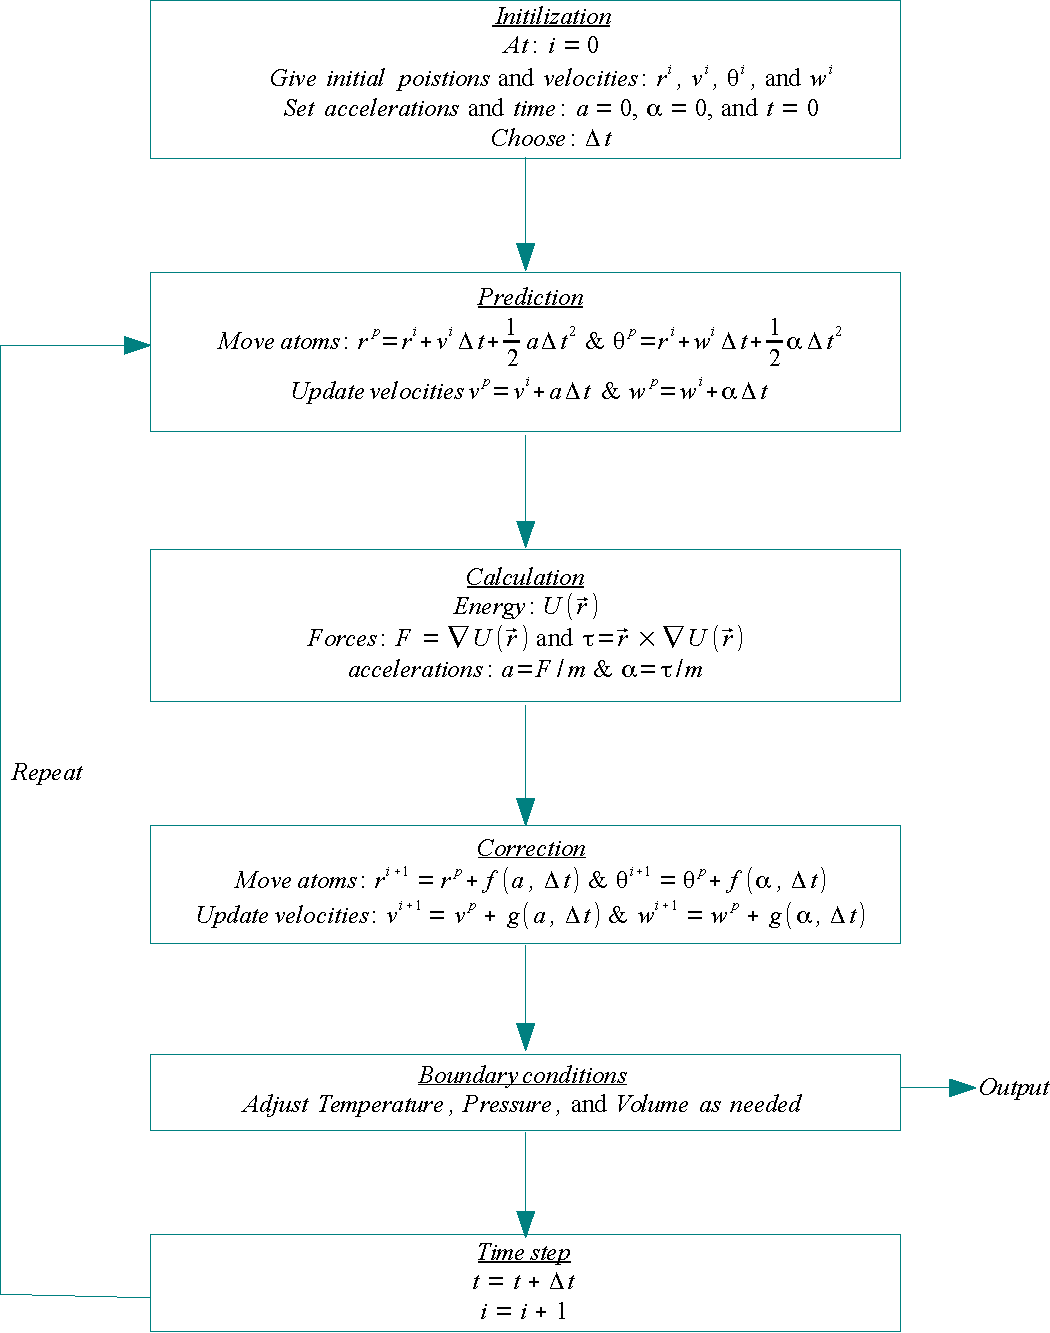
\includegraphics[width = \linewidth]{MD_flowchart.pdf}}
    \caption{Schematic figure showing the step-by-step process in Molecular dynamics simulation.}% where $r, v, \; \mathrm{and}\; a$ are linear position, velocity, and acceleration. and $%theta, %omega, \;\mathrm{and}\; %alpha$ .}are angular position, velocity, and acceleration respectively.% Similarly, $U, F, and %tau$ are energy, force, and torque respectively. The functions $f$ and $g$ evaluates correction factor for position and velocity using acceleration and time step.}
    \label{fig:MD}
  \end{center}
\end{figure}

In a MD simulation, all molecules are initialized by assigning their initial positions and velocities using appropriate boundary conditions. Molecules are usually initialized in such a way so that system does not take too long time to reach equilibrium. Before moving a molecule in the system, the computer must evaluate force and the potential energy contributed by intramolecular interactions as well as intermolecular interactions. The potential energy of the molecule in the system can be written as:
\begin{equation}
U(\mathbf r) = \overbrace{U_{bond} + U_{bend} + U_{torsion}}^{Intramolecular\; interactions} + \overbrace{U_{electrostatic} + U_{van\;der \;Waals}}^{Intermolecular\;interactions} + ...
\label{eq:potential}
\end{equation}   
The force and torque acting on the molecule can be calculated using following equations:

\begin{subequations}
\begin{gather}
\mathbf F = \nabla_r U(\mathbf r, \hat{u}) \\
\mathbf {\mathbf{\tau}} = \mathbf r \times \nabla_r U(\mathbf r, \hat{u}),
\end{gather}
\label{eq:forceTorque}
\end{subequations}
where $\hat{u}$ is the orientation of the molecule and the evaluation of force and torque depends on the direction of orientation for the point multipoles. The force and torque are required to propagate the dynamics to the molecule at a given time step. The same process can be repeated for every molecule in the system. Once every molecule in the system is moved forward a time-step, their positions and velocities are adjusted according to applied boundary conditions (i.e temperature, pressure, volume, etc are adjusted). After adjusting positions and velocities, we can recalculate the potential energy for each molecule and repeat same process until the simulation completes the allowed simulation time.
 
In MD simulations, the intermolecular interactions are the most expensive part of simulation. Among them, the van der Waals interactions are short-range interactions and are often described by Lennard-Jones (LJ) potential:

\begin{equation}
U_{LJ}(r) = 4\epsilon \left[\left(\frac{\sigma}{r} \right)^{12} - \left(\frac{\sigma}{r} \right)^6\right],
\label{eq:LJ}
\end{equation}
where $\sigma$ is diameter of a molecule and $\epsilon$ determines well depth of the attractive potential. The $1/r^6$ in the Eq.~(\ref{eq:LJ}) is short-ranged. The $1/r^{12}$ repulsive part of the  LJ potential prevents two or more molecules from occupying the same position. The electrostatic interactions are considered long-range interactions e.g. charge-charge interactions between molecules can be described by Coulomb's law: 

\begin{equation}
U_{electrostatic}(r) = \frac{1}{4\pi \epsilon_o}\frac{q_1 q_2}{r}.
\label{eq:Coulomb}
\end{equation}
Electrostatic interactions decay much slower with the distance. For charge-charge, they fall off as $ \frac{1}{r}$. If the lowest order moment in the molecule is a dipole, the electrostatic interaction will falls off by ${1}/{r^3}$. Even if the lowest order moment in molecule is a quadrupole, the electrostatic interaction will decay by ${1}/{r^5}$ which is longer range than LJ interaction. Since the electrostatic interaction decays slowly, we need to consider a large number of molecules around it to capture physical behavior due to interactions. Consideration of interactions with large number of molecules is not computationally efficient. The most important challenge in the molecular dynamics communities have been to capture right electrostatic behavior of a molecule considering only its interaction with a small number of neighboring molecules. There have been many efforts to develop efficient and accurate algorithms to evaluate electrostatic interaction in molecular simulation, which will be discussed in detail in section~\ref{sec:ElectMethod}.  

%The main purpose of our research is developing accurate and efficient electrostatic interaction methods considering small number of molecules around a given molecules.  
 
\subsection{Peridic Boundary Condition (PBC)}
Real liquid systems consist of very large number of molecules. But for computational efficiency, only a small number of particles ($\sim 10^3$) are usually considered in molecular simulations. On the other hand, if we want to study and predict bulk properties of the material using small number of molecules, a large fraction of molecules will be near the edge of the sample, contributing a huge surface effect. To eliminate surface effects, Periodic Boundary Conditions (PBC) have long been employed in various molecular simulations.\cite{Born1912}
In PBC, the simulation box is replicated throughout the space to form an infinite lattice. In the course of simulation, if a molecule moves in the central box, its images in replicated boxes will also move in the similar fashion. Similarly when a molecule leaves the central box, one of its images will enter the box through opposite face to conserve total number of particle in a central box (see Fig.~\ref{fig:PBC}). Therefore the system acts like there is no wall at the boundary of the central box and eliminates the surface effect in the computation. If we want to evaluate potential energy of a molecule, we can consider its interactions with nearest molecules or images using the minimum image convention.\cite{Allen04} Even for minimum image convention, we need to calculate large number of pairwise distances at every time step. Consider a system of N molecules, the potential energy of $i^{th}$ molecule we need to find its distances $r_{ij}$ with every $j^{th}$ molecules or images in the system. Therefore in total we need to calculate $\frac{1}{2} N (N-1)$ number of distinct distances at every time-step, which can make the computation very expensive. 

  
\begin{figure}[tpb]
  \begin{center}
    \centerline{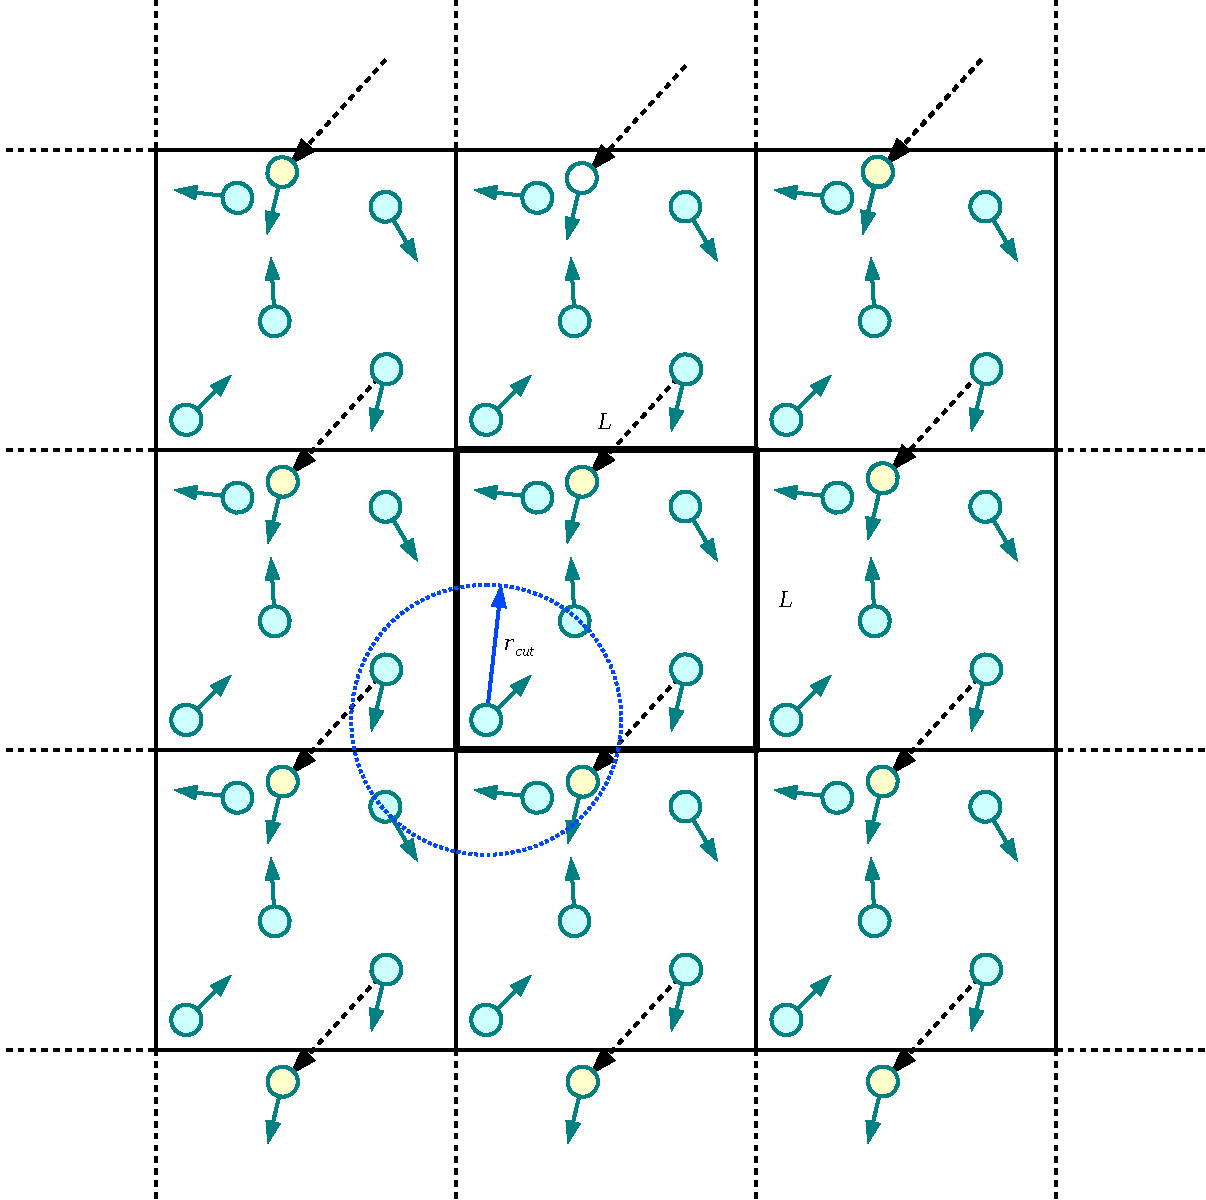
\includegraphics[width = \linewidth]{PBC.pdf}}
    \caption{Periodic Boundary Condition for two dimensional (2D) molecular system. The central 	box is outlined using thicker line and replicated throughout the plane to form a 2D lattice. Usually in molecular simulations, the potential energy of the molecule is evaluated considering its interactions with the molecules or their images located in the spherical cutoff region as shown in blue dotted-circle.}
    \label{fig:PBC}
  \end{center}
\end{figure}

\subsection{Spherical truncation and Neighbor lists }
If we assume the interaction between molecules is short-ranged, we can select small region around the molecule and consider that molecule only interacts with other molecules within that region. Often simulations use small cutoff regions around the molecule in order to make the MD simulation efficient. Beyond the cutoff region there is no interaction between the molecules. Consider a system of $N$  molecules with box size $L$. If PBC is employed, $r_{cut}$ should be less than $L/2$ in the molecular  simulation. If $r_{cut} > L/2$, a molecule may interact with another molecule as well as its own image at the same time, which can lead to spurious correlations in molecular dynamics simulation. The spherical truncation implemented in PBC is shown in Fig.~\ref{fig:PBC}. 

But evaluating all pair distances $r_{ij}$ at every time step for determining whether or not a particular molecule is within cutoff region makes simulation computationally expensive. Therefore cutoff sphere $r_{cut}$ is surrounded by the another larger sphere of radius $r_{list}$ as shown in Fig.~\ref{fig:neighbourList}. At the beginning of the simulation a list of the molecules, the neighbour list, is constructed around each molecule. For a few time steps, only the molecules in the neighbour list are selected to check whether or not molecule is within the cutoff sphere. After a few time steps, the neighbour list is reconstructed by evaluating pair distances between every molecules. This reconstruction time is mainly determined by the dynamics of the molecules in the simulation.  
\begin{figure}[tpb]
  \begin{center}
    \centerline{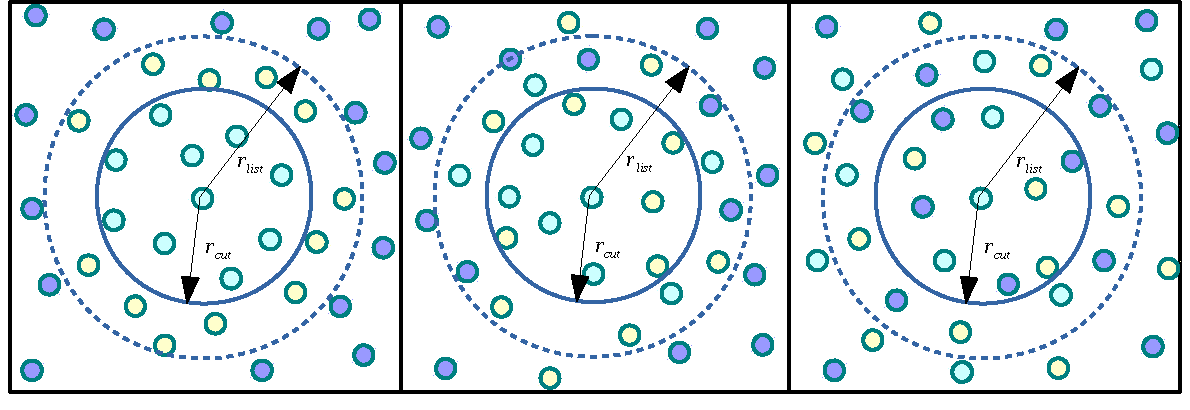
\includegraphics[width = \linewidth]{neighbourList.pdf}}
    \caption{Region of neighbor list around the cutoff sphere. Molecules in the cutoff region, neighbour list, and outer region are indicated by green, yellow, and violet circles respectively. The neighbour list  should be reconstructed before molecules in the outer region starts to penetrate the cutoff region.}
    \label{fig:neighbourList}
  \end{center}
\end{figure}


\section{Monte Carlo (MC) Simulation}
We need to sample a large number of different configurations to study any physical and statistical properties of the system. These configurations must take into account the ensemble being simulated. The Monte Carlo method uses probabilistic sampling of the system to generate representative configurations of the system. Each configuration depends only upon its predecessor but does not depend on the all the other configurations that were visited previously. For a canonical system, the probability of obtaining a given configuration is given by Boltzmann factor, $\mathrm{exp}(-{\Delta E}/{k_B T})$. Metropolis \textit{et.al} developed the selection criteria for acceptance of the subsequent configuration of the system. \cite{Metropolis53} According to their method, the new configuration of the system is accepted either  $\Delta E < 0$ or  $e^{-\frac{\Delta E}{k_B T}} > r$, where $r$ is the random number between 0 and 1. The evaluation of the potential energy difference between subsequent configurations, $\Delta E$, is very important in the MC simulation. For computational efficiency, this method also utilizes cutoff region $r_{cut}$ as well as periodic boundary condition to calculate electrostatic interaction. Therefore developing an efficient and accurate electrostatic interaction method has always been subject of interest in the MC community. 

\section{Electrostatic Methods}
\label{sec:ElectMethod}
Consider a system of $N$ particles in a cubic box of length $L$  replicated infinitely in 3D-space. The electrostatic potential energy for a particle with charge $q_i$ and position $r_i$ is given by
\begin{equation}
U_i =  \sum_n{}^{'}{ \sum_{j=1}^N {\frac{q_i q_j}{\lvert {\mathbf{r}_i-\mathbf{r}_j + \mathbf{n}L}\rvert}}},
\label{eq:electrostatic}
\end{equation}
where $q_j$ represents all other charges located at position $\mathbf{r}_j$ or in periodic replica and $\mathbf{n}$ is the cell-coordinate vector, $\mathbf{n}L = n_1 L \;\hat{x} + n_2 L\;\hat{y} + n_3 L\;\hat{z}$, where integers $n_1,n_2, \text{and}\; n_3$ number cells along the $x$, $y$, and $z$ directions and vary from 0 to $\infty$. The prime in the first sum indicates that $i =j $ should be ignored for the central box, i.e. $n = 0$. The factor ${1}/({4\pi\epsilon_o})$ has been dropped in the Eq.~(\ref{eq:electrostatic}) for simplicity. The total potential energy of the system can be calculated as,
\begin{equation}
U = \sum_{\substack{i=1 \\ i\neq j}}^N{U_i} = \frac{1}{2}\sum_n{}^{'}{\sum_{i=1}^N { \sum_{j=1}^N {\frac{q_i q_j}{\lvert {\mathbf{r}_i-\mathbf{r}_j + \mathbf{n}L}\rvert}}}},
\label{eq:totalElectrostatic}
\end{equation}
where factor of ${1}/{2}$ in the second part of the Eq.~(\ref{eq:totalElectrostatic}) is due to removal $i \neq j$ in the summation.
 
As we know the electrostatic interaction is a long-range interaction which is time consuming. On the other hand the potential energy evaluated using Eq.~(\ref{eq:electrostatic}) converges conditionally to the correct value depending on the order of summation taken into account during  calculation.\cite{Allen89} Therefore there have been many efforts to reduce computational cost and remove its conditionally convergent behavior.  

\subsection{Ewald Method}
The Ewald method was originally proposed by \texit{Ewald} in 1921 to evaluate electrostatic interactions in PBC. In this method, the electrostatic interaction  can divided into two rapidly converging real and reciprocal space sums as well as a constant self-term. \cite{Toukmaji96} Since  $\mathrm{erf}(x) + \mathrm{erfc}(x) = 1$ we can write Eq.~(\ref{eq:totalElectrostatic}) as,

\begin{equation}
U = \frac{1}{2}\sum_n^{'}{\sum_{i=1}^N { \sum_{j=1}^N {q_i q_j}}}\frac{\mathrm{erfc}(\alpha r_{ij,n})+\mathrm{erf}(\alpha r_{ij,n})}{r_{ij,n}}.
\label{eq:errorFuncElectrostatic}
\end{equation} 
The real-space term~\ref{eq:ewald1} in Ewald method is obtained by taking complementary error function term in the Eq.~(\ref{eq:errorFuncElectrostatic}). Similarly reciprocal-space part~\ref{eq:ewald2} can be obtained by taking Fourier transform of the error function term in Eq.~(\ref{eq:errorFuncElectrostatic}). The self-term present in the equation removes artificial interactions of the charge with its own images located in the periodic replicas. 

\begin{subequations}
\begin{gather}
U_{real} = \frac{1}{2} \sum_{i,j}^{N}{\sum_{n}^{'}{{q_i q_j}\frac{\mathrm{erfc}(\alpha r_{ij,n})}{r_{ij,n}}}}, \label{eq:ewald1}\\
U_{reciprocal} = \frac{1}{2\pi V}\sum_{i,j}^{N}{\sum_{\mathbf{m} \neq 0}\frac{\exp(-(\pi \mathbf{m}/\alpha)^2 + 2\pi i \mathbf{m}\cdot{\mathbf{r}_{ij})}}{\mathbf{m}^2}},\label{eq:ewald2} \\
U_{self} = -\frac{\alpha}{\sqrt{\pi}} \sum_{i =1}^{N} {q_i}^2 ,\label{eq:ewald3}
\end{gather}
\end{subequations}
where $V$ is the volume of the simulation box, $\mathbf{m}$ is a reciprocal-space vector, and $\alpha$ is a damping parameter which determines the rate of convergence in the real and reciprocal space. 
 
Physically each point charge in the system can be assumed to be surrounded by a Gaussian distribution of equal magnitude but oppositely-signed charge (see Fig.~\ref{fig:Ewaldsum}) with density,

\begin{equation}
\rho_i (r) = q_i \left(\frac{\alpha}{\sqrt{\pi}}\right)^3 \exp(-\alpha^2 r^2),
\label{eq:chargeDistribution}
\end{equation}
where $\alpha$ is a damping parameter determines the distribution of the charge, and $r$ is the distance from the center of distribution. The imposed charge distribution around a charge screens the interactions between the charges making the effective interaction  short ranged and therefore converges rapidly with distance. These Gaussian distributions are counteracted by other Gaussian distributions of charge having same magnitude but opposite sign as shown in Fig.~\ref{fig:Ewaldsum}. \cite{Toukmaji96} The sum of potential energy due to second type of charge distributions converges in reciprocal space. 

\begin{figure}[tpb]
  \begin{center}
    \centerline{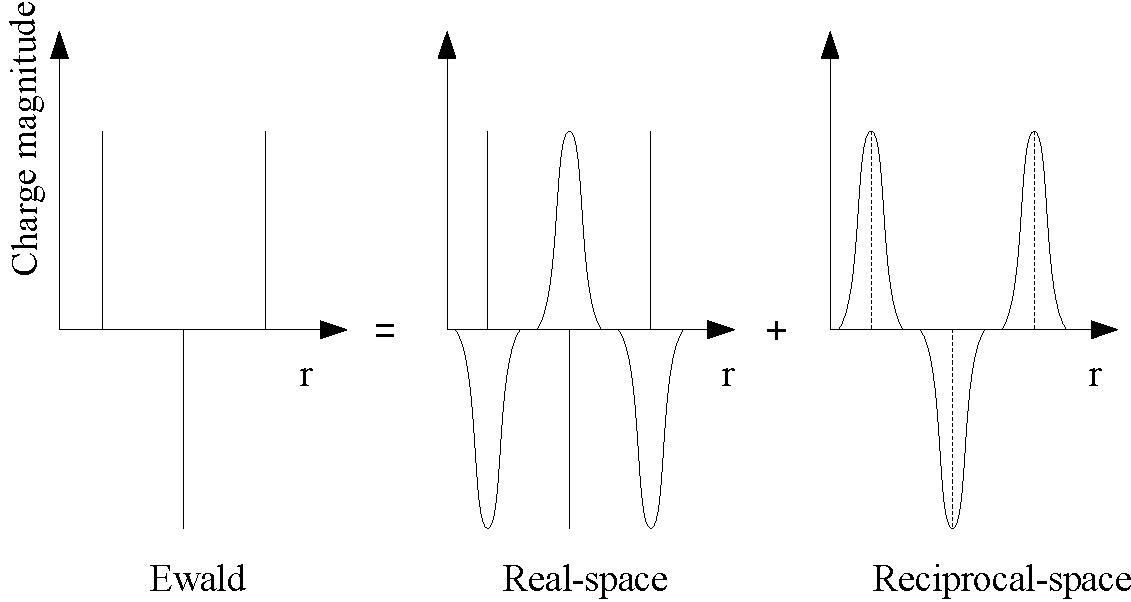
\includegraphics[width = \linewidth]{Ewaldsum.pdf}}
    \caption{In the Ewald method each point charge is surrounded by a Gaussian distribution of equal and oppositely-signed charge, evaluated in real-space. These Gaussian distributions are compensated by the opposite-singed Gaussian distribution of the charges calculated in reciprocal-space }
    \label{fig:Ewaldsum}
  \end{center}
\end{figure}

In the minimum image convention scheme, each particle can interact with its nearest particles or their image, the total number of interactions is $\frac{1}{2}N(N-1)$ in Ewald method. Therefore the algorithmic complexity for the Ewald method is $O(N^2)$. Recerz and Jacobs suggested that by choosing proper simulation parameters and minimum image convention schemes we can make reciprocal potential very small as compared to real-space potential so that can be ignored.\cite{Jacobs92} However this method is only applicable for a larger system but contribution of the reciprocal-space sum might not small for all systems, therefore is not recommended for general MD simulations. Perram \textit{et al.} subdivided each simulation box into $m \times m \times m$ sub-boxes and selected damping parameter $\alpha = m \sqrt{-\log(\delta)}$ , where $\delta$ is the relative error constant for neglecting the maximum term in the real-space sum, and using this technique they were able to reduce computational time   to $O(N^{3/2})$.

\subsection{Fourier-based Ewald Methods}
The Ewald method has been further modified using Fast Fourier transforms (FFT) to reduce complexity to $O(N\log(N))$. In these methods, charges are interpolated onto a 3D grid and the reciprocal sum is evaluated using FFTs. The particle-particle particle-mesh Ewald (PPPME) and particle-mesh Ewald (PME) methods are two widely-used Fourier-based Ewald methods. 

\begin{figure}[tpb]
  \begin{center}
    \centerline{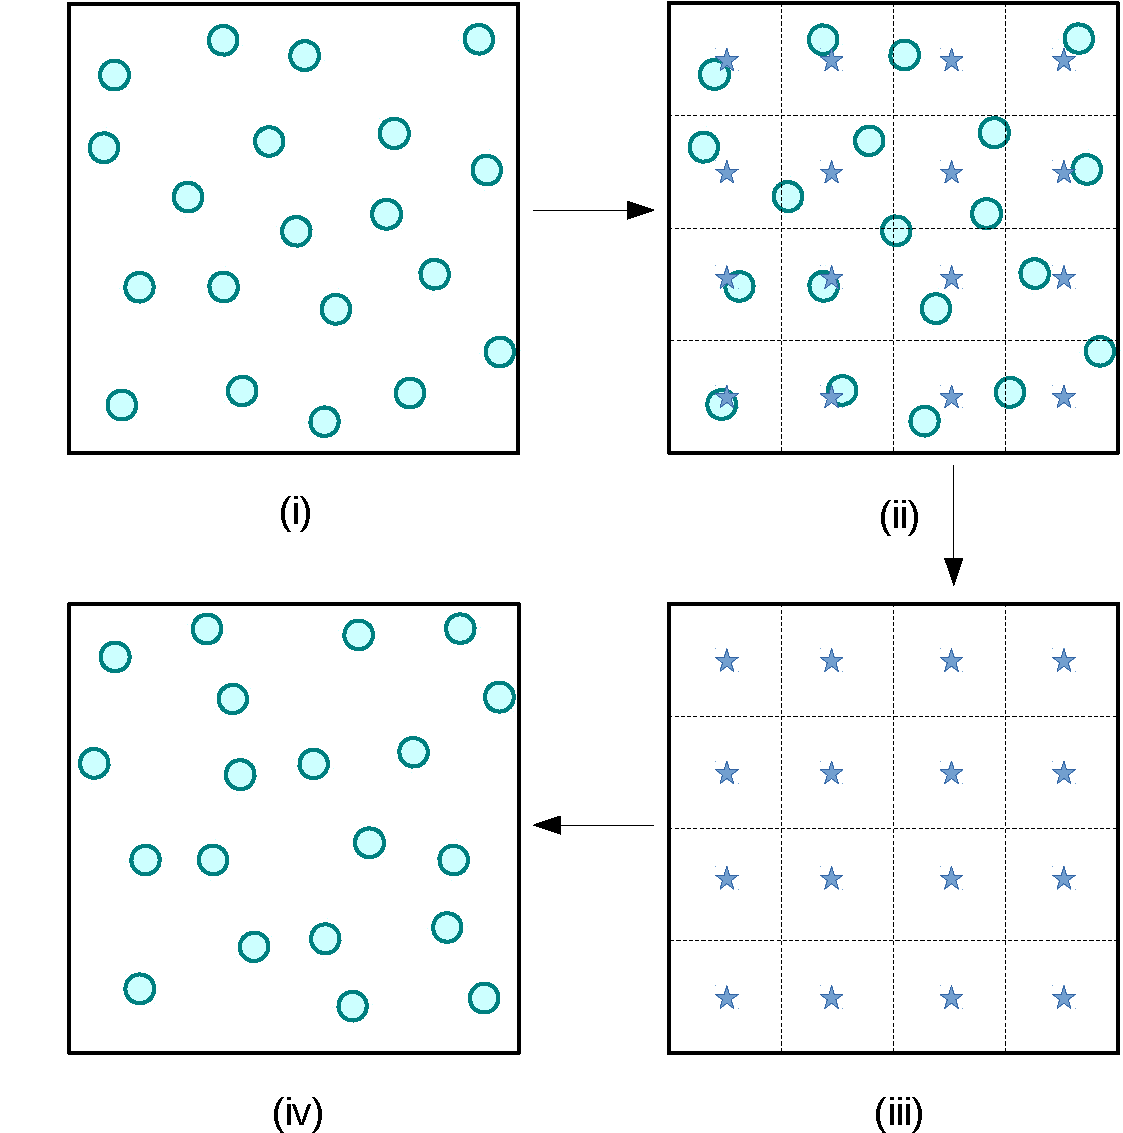
\includegraphics[width = \linewidth]{PM_method.pdf}}
    \caption{Schematic diagram for Fourier-based Ewald methods where green circle represents charge and blue star denotes grid point. In the Figs., (i) a system of charges, (ii) charges mapped with grid points, (iii) force evaluated at the grid points, and (iv) force mapped back to the particles and their positions and velocities are updated. }
    \label{fig:PPPME}
  \end{center}
\end{figure}
\subsubsection{Particle-Particle Particle-Mesh Ewald (PPPME)}
\label{subsec:PPPME}
The PPPME method was originally developed by Hockmney and Eastwood \cite{Hockney88} and extended  by Luty \textit{et al.}.\cite{Luty94} and Rajagopal \textit{et al.} \cite{Rajagopal94} In this method, the electrostatic interaction is divided into short-ranged real-space and long-ranged reciprocal-space sums. The charges in the system are approximated as uniformly decreasing spherical charge density. The short-ranged potential within the cutoff radius $r < r_{cut}$ is calculated using electrostatic interactions between charge distributions. To calculate the long-ranged potential, first of all charges are assigned to the 3D grid as shown in Fig.~\ref{fig:PPPME} and transformed to the Fourier space for evaluating electrostatic potential. Since charges are assigned to the grid, it is very efficient to calculate electrostatic interactions in reciprocal space. Once the potential energy is evaluated, an inverse Fourier transformation is applied to calculate energy in real-space and it is numerically differentiated to get the force acting on the grid. Finally the electrostatic force (or energy) can be interpolated from the grid onto the particle locations to obtain actual force acting on the particle.

Although PPPME has complexity of $O(N \mathrm{log}N)$, for computational accuracy, we either need to refine the mesh or use better interpolation techniques, both of which are computational expensive. In addition to this, using numerical differentiation to calculate forces may introduce errors in the calculation. Therefore higher order differentiation schemes are often used in force calculations. In order to get optimal performance, all of the parameters; charge-distribution, interpolation technique, and differentiation schemes must be properly selected for a given system making  parameter choices system specific. \cite{Toukmaji96}

\subsubsection{Particle-Mesh Ewald (PME)}
\label{subsubsec:PME}
This method is the modification of the PPPME method, in which the potential energy is divided into real-space and reciprocal-space sums. The charge is represented by the Gaussian distributions of charge. In this method, the real-space sum within the cutoff sphere is evaluated using actual electrostatic interactions between charges whereas the reciprocal sum is calculated in Fourier space using the idea of 3D grid as explained in the PPPME method. Unlike PPPME, this method evaluates force analytically, differentiating electrostatic energy at a given grid point reducing memory requirement significantly. This method also has $O(N\mathrm{log}N)$ algorithmic complexity and uses interpolation to map back electrostatic force from grid to the particle's location. Therefore users of this method need to discover optimal interpolation schemes to obtain excellent speed and accuracy for a simulation, making this method system dependent.

\subsection{Real Space Methods}
Before discussing the real space methods, the fundamental property of the electrostatic interactions in condensed phase environments should be considered. The electrostatic interaction between two charged particles decays as $1/r$. But molecular systems are usually composed of an equal number of positive and negative charges. Thus the range of interaction between a particular charge and rest of the charges in the system are different than the interaction between two bare charges. Consider a one dimensional (1D) crystal lattice composed of positive and negative charges. The potential energy of a particular ion can be considered as a sum of interactions with positive and negative ion pairs as shown in Fig.~\ref{fig:schematic}(a). Mathematically the potential energy for 1D crystal with alternating charges is given by a Madelung sum,

\begin{equation}
\begin{split}
U^{Mad} & = -2q_iq_j\left(\frac{1}{a}-\frac{1}{2a}\right)-2q_iq_j\left(\frac{1}{3a}-\frac{1}{4a}\right)-2q_iq_j\left(\frac{1}{5a}-\frac{1}{6a}\right) + ... \\
		& = -\left(\frac{ 2q_iq_j}{(1.414)^2a}\right)-\left(\frac{2q_iq_j}{(3.464)^2a}\right)-\left(\frac{2q_iq_j}{(5.477)^2a}\right) +...
\end{split}
\label{eq:1D}
\end{equation} 
 
\begin{figure}
  \centering
  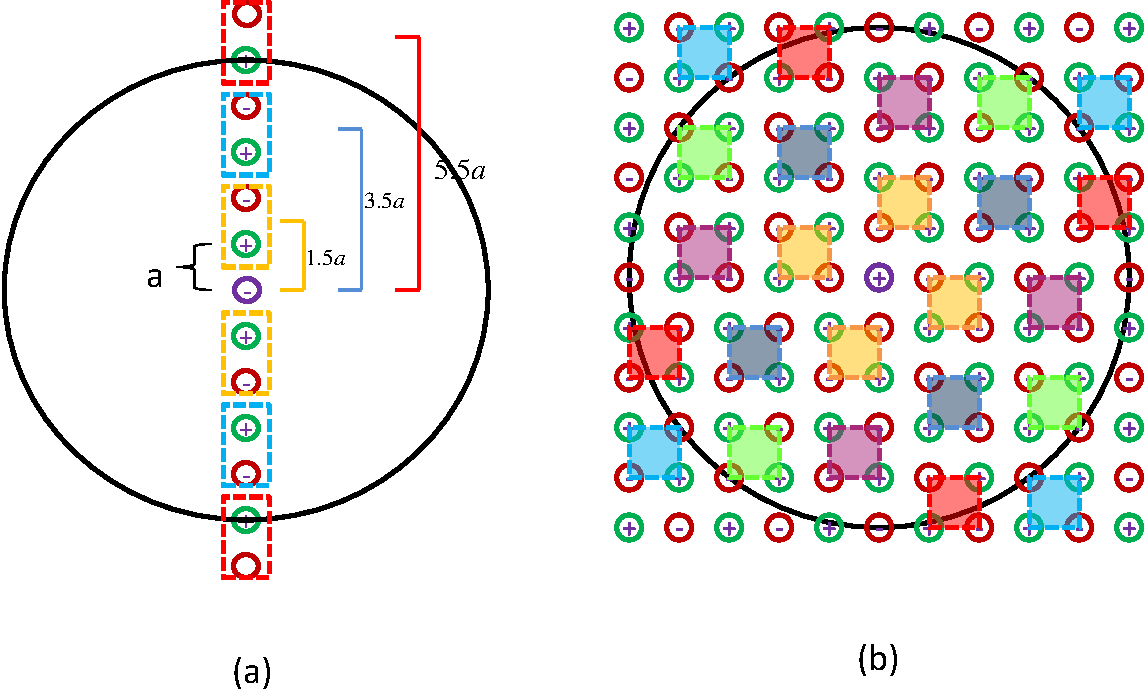
\includegraphics[width=\linewidth]{1D_2DCrystal.pdf}
  \caption{Schematic diagram showing grouping of ions in (a) 1D (b) 2D crystals. The interaction of the central ion with the group of ions decays faster than $1/r$. The direct spherical truncation breaks the ordering of the ions at the cut off sphere providing a net charge within the cutoff sphere. The breaking of the charge ordering increases with the crystal dimension resulting in a large net charge in the higher dimensional crystal.}
   \label{fig:schematic}
\end{figure}

If we consider all 3 terms in the Eq.~(\ref{eq:1D}) and compare their distances with the distance between central ion and group of ions as shown in Fig.~\ref{fig:schematic}(a), we clearly see that the interaction energy of a single ion with the pairs converges faster than ($1/r$). Similarly, in a two dimensional (2D) lattice, the potential energy of an ion can be described as a sum of positive and negative four body groups as seen in Fig.~\ref{fig:schematic}(b). The interaction energy between an ion and group of four ions decays much faster than the charge-charge interaction. For a three-dimensional (3D) crystal, the potential energy of an ion can be considered as due to its interaction with the group of eight ions forming a cube. From this generalization, we can conclude that the electrostatic interaction energy for an ion in the crystalline system is a short-ranged as compared to charge-charge interaction. Therefore, even the relatively small systems should be able to represent bulk long-ranged interactions.


In order to reduce the computational expense of a molecular dynamics simulation, interactions between particles are only considered if the particles exist within a cutoff distance $r_c$, of one another. We first consider how the energy of a system behaves if we truncate the interactions at the cutoff radius.  Fig.~\ref{fig:energyVsCutoff} shows (black line) that the electrostatic potential energy does not converge to the Madelung energy upon increasing the cutoff radius for the direct truncation. On the other hand the energy is found to be closer to the Madelung constant when the net charge within the cutoff radius is zero (Fig.~\ref{fig:energyVsCharge}). This oscillation in the potential energy is due to the breaking in charge ordering on the surface of the cutoff sphere which results in a net charge within the cutoff sphere. The size of the net charge is proportional to the dimension of the crystal. Although the interaction energy is short ranged,  the direct truncation results in severe oscillation in energy for 3D crystal as shown in Fig.~\ref{fig:energyVsCutoff}. Dipolar (or quadrupolar) crystals are also formed by ordering of the dipolar (or quadrupolar) molecules. Therefore similar oscillatory behaviour in the potential energy is due to the breaking of the ordering of dipoles (or quadrupoles) on the surface of the truncated sphere. Even in liquids there is local ordering of the molecules due to electrostatic interaction and similar oscillatory behaviour in the electrostatic potential has been seen in direct truncation approaches.

\begin{figure}[tpb]
  \begin{center}
    \centerline{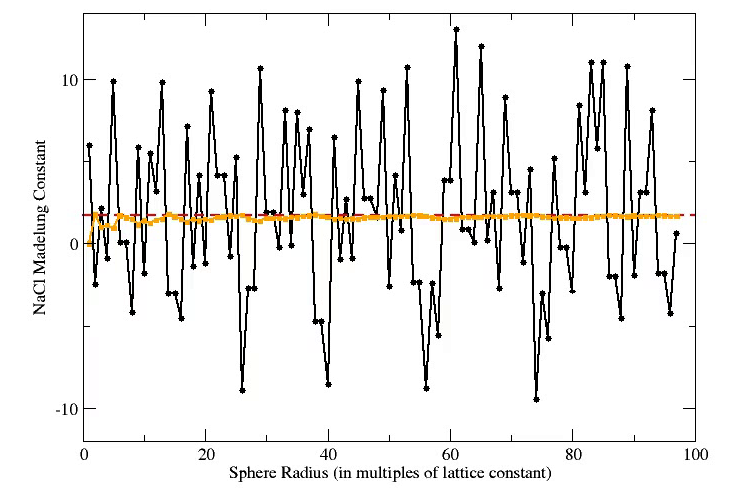
\includegraphics[width = \linewidth]{energyVsCutoff.png}}
    \caption{Convergence of the lattice energy constants for a 3D NaCl crystal as a function of cutoff radius for the direct (hard) cutoff method (black line). The orange line in the figure is for charge neutralized cutoff sphere (when image charge placed on the surface of the cutoff sphere). The red dotted line represents Madelung energy for NaCl crystal}
    \label{fig:energyVsCutoff}
  \end{center}
\end{figure}

\begin{figure}[tpb]
  \begin{center}
    \centerline{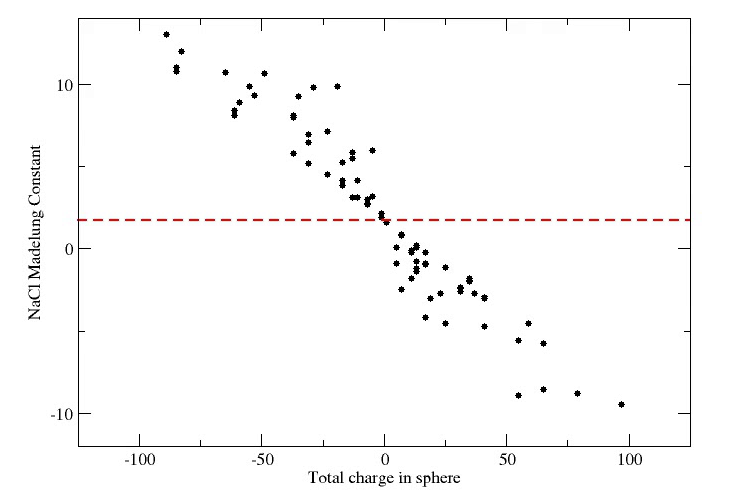
\includegraphics[width = \linewidth]{energyVsNetcharge.png}}
    \caption{Convergence of the lattice energy constants for the NaCl crystal as a function of net charge within a cutoff sphere. The red dotted line represents Madelung energy for NaCl crystal}
    \label{fig:energyVsCharge}
  \end{center}
\end{figure}
Wolf \textit{et al} \cite{Wolf99} proposed the idea of placing an image charge on the surface of cutoff sphere for every charge found within the sphere. The image charges should have opposite charge of those found within the sphere guaranteeing charge neutralization  within the cutoff sphere.\cite{Wolf99} This charge neutralization converges the potential energy to the correct Madelung energy as shown in Fig.~\ref{fig:energyVsCutoff} (orange line). In molecular dynamics (MD) simulations, the energy, force and torque should approach zero as the distance between molecules approaches the cutoff radius  in order to conserve total energy. However Wolf's forces and torques derived from the potential do not go to zero at the cutoff radius, which makes it inappropriate to use in MD simulations. More recently, Zahn \textit{et al.} and Fennell and Gezelter proposed the damped shifted force (DSF) potential, which incorporates Wolf's approach of image charges while ensuring the forces and torques approach zero at the cutoff radius.\cite{Zahn02, Gezelter06} Fukuda has also recently been successful with the neutralization of higher order moments in a system of point charges.\cite{Fukuda13}

Real-space methods scale linearly with system size, are system-independent, and applicable a variety of condensed phase environments. Therefore we selected real-space methods for extending to higher-order charge-multipoles. In our research, we have generalized Wolf's shifted potential (SP) to the higher order electrostatic multipoles. We have also developed the gradient shifted force (GSF) and Taylor shifted force (TSF) potentials which are the natural extension of the damped shifted force (DSF) for higher order charge-multipoles. In the following chapter 2, I will discuss the development of the SP, GSF, and TSF methods and evaluate the energy constants for various dipolar and quadrupolar crystals using newly developed methods and compare with analytical results.\cite{Lamichhane14_I} 

%
% Chapter 2
%
%
% Modified by Megan Patnott
% Last Change: Jan 18, 2013
%
%%%%%%%%%%%%%%%%%%%%%%%%%%%%%%%%%%%%%%%%%%%%%%%%%%%%%%%%%%%%%%%%%%%%%%%%
%
% Modified by Sameer Vijay
% Last Change: Wed Jul 27 2005 13:00 CEST
%
%%%%%%%%%%%%%%%%%%%%%%%%%%%%%%%%%%%%%%%%%%%%%%%%%%%%%%%%%%%%%%%%%%%%%%%%
%
% Sample Notre Dame Thesis/Dissertation
% Using Donald Peterson's ndthesis classfile
%
% Written by Jeff Squyres and Don Peterson
%
% Provided by the Information Technology Committee of
%   the Graduate Student Union
%   http://www.gsu.nd.edu/
%
% Nothing in this document is serious except the format.  :-)
%
% If you have any suggestions, comments, questions, please send e-mail
% to: ndthesis@gsu.nd.edu
%
%%%%%%%%%%%%%%%%%%%%%%%%%%%%%%%%%%%%%%%%%%%%%%%%%%%%%%%%%%%%%%%%%%%%%%%%

%
% Chapter 2
%

\chapter{GNU THINGS ARE GOOD THINGS FOR ALL GRADUATE STUDENTS OR SO IT SEEMS}
\label{chap:golfing}

\section{Gnu See, Gnu Do, Gnu Goes Golfing with Green Golf Genes and
  Gesticulates Grapes}

So why do gnus do what they do?  This is a perennial question that has
yet to be answered definitively by scientists.  Is their future
somehow tied inexplicably with that of humans?  Hard to say, but we do
feed them a lot.  It has even been theorized that rotundness is a
symbol of status or class within the Gnus; those who are more
productive (i.e., cute, furry, friendly) will be fed more than those
who are less so.  So the more rotund, the higher status one has in the
Gnu society.

One could extrapolate this to mean that there is a super-Gnu out there
somewhere; the biggest, rotundest Gnu that you've ever seen, probably
of epic proportions!  This would have to be the Leader of Gnus, or LoG
for short.  But the LoG would definitely have to be the cutest,
furriest, and most friendly Gnu that you've ever seen.

\subsection{The LoG}

So how does the LoG get chosen?  Ultimately by humans.  So we can say
that the Gnu society is perhaps the truest democracy that has ever
existed; the leader is chosen by merit, and chosen by complete
outsiders.  As such, the LoG must truly epitomize all that Gnus stand
for: opposedness to overmanagement, cuteness, friendliness, and
furriness~\citep{gloonson98:_gnuly_discov_gnus}.  The gnus themselves
vote at an anual election, based upon these attributes (campagaining
is an anethema to Gnus; see Section~\ref{sec:groovin-gnus}).

\subsubsection{Election Data}
\label{sec:data}

Table~\ref{tbl:votes} shows the latest electoral college voting by the
LoG for the year 2000.  Each Gnu is scored on a scale of one to ten on
the attributes described above.  The results shown in the table are
average scores in each category for all votes; the Gnu's final score
is shown in the final column.

%
% Be aware that page-spanning tables a Very Odd Creatures.  The
% "longtable" environment in LaTeX does some deep Voodoo to make
% everything work out properly.  One of its deep incantations is to
% make the table appear as though it is double spaced.  You can fix
% this by trailing each line with "\\[-6em]" instead of just "\\".
% When using longtable it is also important to compile your file
% more than once. But you're probably already doing this to get
% the internal references correct, anyway.
%

\begin{center}
  \begin{longtable}{lccccc}
    \caption{ELECTORAL COLLEGE RESULTS FOR THE LoG ELECTION IN THE YEAR
2000\label{tbl:votes}\/}\\
        \toprule
        Candidate\footnote{note all names begin with G} & Anti-management & Cuteness & Friendliness & Furriness & Aggregate \\
        \midrule
\endfirsthead % Everything above goes at the top of the 1st page only
% As with the first header, we don't want obscene amounts of space for
% subsequent headings either, and eliminate an em of whitespace.
  \caption[]{{\em Continued}}\\
  \midrule
  Candidate & Anti-management & Cuteness & Friendliness & Furriness & Aggregate \\
  \midrule
\endhead % Everything above here (and below the \endfirsthead) goes at the top
         % of continuation pages.  The [] argument prevents a duplicate
         % entry from appearing in the table of contents.
% The following 3 lines are provided as an example only -- per ND
% guidelines, the footer at the bottom of a page for a longtable
% should not have a bottom line.  Only the absolute bottom of the
% table should have a final \bottomline

%  \midline
%  \multicolumn{6}{|r|}{\textit{continued}\ldots} \\
%  \bottomrule
\endfoot % The above section goes at the bottom of continuation pages
  \bottomrule
\endlastfoot % The very last bottom of the table
    Glen & 6.2 & 7.0 & 6.1 & 9.8 & 7.2 \\
    Goober & 6.9 & 2.1 & 5.7 & 4.1 & 4.6 \\
    Genevra & 2.2 & 2.0 & 1.1 & 1.1 & 1.6 \\
    Greg & 8.3 & 0.4 & 1.1 & 9.5 & 4.8 \\
    Gina & 6.0 & 7.8 & 6.4 & 4.9 & 6.2 \\
    Geof & 1.1 & 8.7 & 3.7 & 7.3 & 5.2 \\
    Grendel & 2.8 & 1.7 & 3.4 & 3.2 & 2.7 \\
    Geronimo & 1.2 & 1.2 & 8.8 & 2.2 & 3.3 \\
    Gabrielle & 4.7 & 3.6 & 0.8 & 2.0 & 2.7 \\
    Giovani & 8.4 & 5.8 & 3.4 & 7.4 & 6.2 \\
    Graham & 4.7 & 5.8 & 5.3 & 0 & 3.9 \\
    Gil & 5.9 & 4.0 & 5.5 & 7.6 & 5.7 \\
    Gerald & 2.0 & 3.7 & 8.0 & 4.3 & 4.5 \\
    Guilani & 7.7 & 3.9 & 2.7 & 6.4 & 5.1 \\
    Guido & 7.6 & 4.3 & 6.5 & 1.0 & 4.8 \\
    Godzilla & 5.1 & 2.2 & 5.3 & 6.9 & 4.8 \\
    Gail & 5.7 & 7.9 & 4.1 & 1.0 & 4.6 \\
    Garth & 4.7 & 7.1 & 2.5 & 3.0 & 4.3 \\
    Gavin & 1.1 & 9.5 & 0.4 & 8.0 & 4.7 \\
    George & 9.5 & 4.5 & 9.1 & 7.5 & 7.6 \\
    Gunnar & 1.4 & 5.8 & 4.8 & 6.2 & 4.5 \\
    Gillian & 7.6 & 9.0 & 6.4 & 4.6 & 6.9 \\
    Greta & 1.5 & 0.5 & 0.9 & 7.7 & 2.6 \\
    Gabby & 1.2 & 3.3 & 7.0 & 2.1 & 3.4 \\
    Gaetena & 6.8 & 1.9 & 4.1 & 8.3 & 5.2 \\
    Ganet & 2.3 & 1.1 & 8.5 & 7.3 & 4.8 \\
    Gardenia & 1.8 & 9.5 & 9.9 & 3.0 & 6.0 \\
    Genna & 5.2 & 3.7 & 3.4 & 3.8 & 4.0 \\
    Genesis & 1.7 & 8.3 & 6.7 & 4.9 & 5.4 \\
    Genaveve & 4.7 & 8.9 & 3.4 & 9.2 & 6.5 \\
    Gene & 3.3 & 6.9 & 0.6 & 5.5 & 4.0 \\
    Gilda & 5.2 & 4.6 & 9.9 & 1.4 & 5.2 \\
    Goldie & 8.9 & 9.1 & 2.0 & 8.2 & 7.0 \\
    Grace & 5.9 & 3.2 & 3.1 & 4.3 & 4.1 \\
    Gretchen & 4.5 & 6.5 & 1.6 & 1.3 & 3.4 \\
    Garrick & 4.8 & 5.7 & 9.4 & 5.1 & 6.2 \\
    Gallagher & 7.4 & 0.4 & 7.6 & 0.4 & 3.9 \\
    Gerry & 1.4 & 8.8 & 4.7 & 0.5 & 3.8 \\
    Gertrude & 9.1 & 8.3 & 0.4 & 5.5 & 5.8 \\
    Gehosephet & 6.6 & 2.9 & 8.3 & 4.4 & 5.5 \\
    Gohn & 8.7 & 2.6 & 7.4 & 2.3 & 5.2 \\
    Gibby & 8.7 & 6.9 & 4.7 & 7.2 & 6.9 \\
  \end{longtable}
\end{center}

As you can see from Table~\ref{tbl:votes}, George (my favorite Gnu)
won for the year 2000, with an aggregate score of 7.6.

% % uncomment the following lines,
% if using chapter-wise bibliography
%
% \bibliographystyle{ndnatbib}
% \bibliography{example}

%
% Chapter 3

%
% Modified by Megan Patnott
% Last Change: Jan 18, 2013
%
%%%%%%%%%%%%%%%%%%%%%%%%%%%%%%%%%%%%%%%%%%%%%%%%%%%%%%%%%%%%%%%%%%%%%%%%
%
% Modified by Sameer Vijay
% Last Change: Wed Jul 27 2005 13:00 CEST
%
%%%%%%%%%%%%%%%%%%%%%%%%%%%%%%%%%%%%%%%%%%%%%%%%%%%%%%%%%%%%%%%%%%%%%%%%
%
% Sample Notre Dame Thesis/Dissertation
% Using Donald Peterson's ndthesis classfile
%
% Written by Jeff Squyres and Don Peterson
%
% Provided by the Information Technology Committee of
%   the Graduate Student Union
%   http://www.gsu.nd.edu/
%
% Nothing in this document is serious except the format.  :-)
%
% If you have any suggestions, comments, questions, please send e-mail
% to: ndthesis@gsu.nd.edu
%
%%%%%%%%%%%%%%%%%%%%%%%%%%%%%%%%%%%%%%%%%%%%%%%%%%%%%%%%%%%%%%%%%%%%%%%%

%
% Chapter 3
%

\chapter{COMPARISONS WITH THE EWALD SUM}
\label{chap:compEwald}

In the previous chapter, I briefly discussed the short-ranged nature of the electrostatic interaction in the crystalline environment. This chapter discusses the property of the electrostatic interactions in more detail and extend the idea of the short-ranged nature of the interaction in the case of liquid simulation. I present the comparison of the energies, forces and torques calculated using real-space methods with the Ewald sum. Additionally I derive different static and dynamic properties using newly developed real-space methods and compare result with the Ewald. Finally I report on the conservation of total energy in the molecular dynamics simulation for the various real-space and Ewald methods.  

\section{Introduction}

As we mentioned earlier Wolf \textit{et al.}\cite{Wolf99} proposed a real space $O(N)$ method for calculating electrostatic interactions between point charges. They argued that the effective Coulomb interaction in most condensed phase systems is effectively short
ranged.\cite{Wolf92,Wolf95} For an ordered lattice (e.g., when
computing the Madelung constant of an ionic solid), the material can
be considered as a set of ions interacting with neutral dipolar or
quadrupolar ``molecules'' giving an effective distance dependence for
the electrostatic interactions of $r^{-5}$ (see Fig.~\ref{fig:schematic1}). If one views the \ce{NaCl} crystal as a simple
cubic (SC) structure with an octupolar \ce{$\mathrm{(NaCl)_4$}} basis, the
electrostatic energy per ion converges more rapidly to the Madelung
energy than the dipolar approximation.\cite{Wolf92} To find the
correct Madelung constant, Lacman suggested that the NaCl structure
could be constructed in a way that the finite crystal terminates with
complete \ce{$\mathrm{(NaCl)_4$}} molecules.\cite{Lacman65} The central ion sees
what is effectively a set of octupoles at large distances. These facts
suggest that the Madelung constants are relatively short ranged for
perfect ionic crystals.\cite{Wolf99} For this reason, careful
application of Wolf's method can provide accurate estimates of
Madelung constants using relatively short cutoff radii.

Direct truncation of interactions at a cutoff radius creates numerical
errors.  Wolf \textit{et al.} suggest that truncation errors are due
to net charge remaining inside the cutoff sphere.\cite{Wolf99} To
neutralize this charge they proposed placing an image charge on the
surface of the cutoff sphere for every real charge inside the cutoff sphere. These charges are present for the evaluation of both the pair
interaction energy and the force, although the force expression
maintains a discontinuity at the cutoff sphere.  In the original Wolf
formulation, the total energy for the charge and image were not equal
to the integral of the force expression, and as a result, the total
energy would not be conserved in molecular dynamics (MD)
simulations.\cite{Zahn02} Zahn \textit{et al.}, and Fennell and
Gezelter later proposed shifted force variants of the Wolf method with
commensurate force and energy expressions that do not exhibit this
problem.\cite{Zahn02,Gezelter06} Related real-space methods
were also proposed by Chen \textit{et al.} \cite{Chen04,Chen06,Denesyuk08,Rodgers06}
and by Wu and Brooks.\cite{Wu05} Recently, Fukuda has successfully
used additional neutralization of higher order moments for systems of
point charges.\cite{Fukuda13}

\begin{figure}
  \centering
  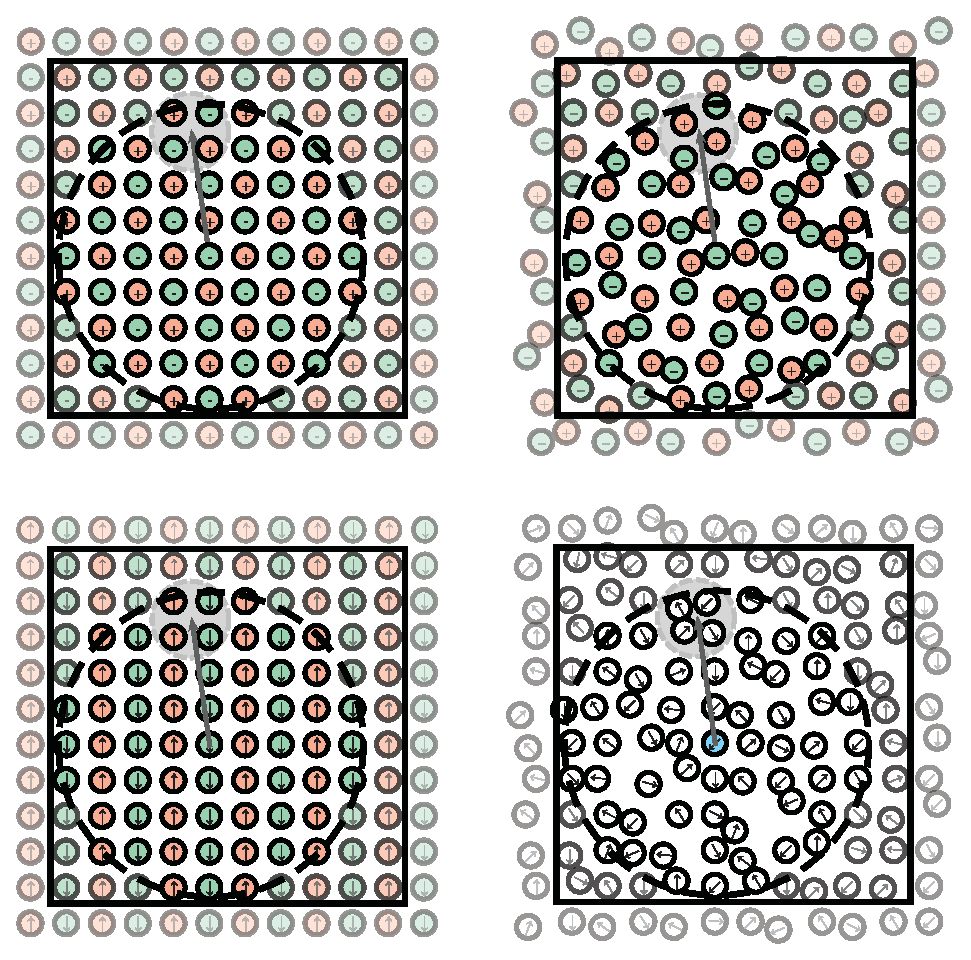
\includegraphics[width=\linewidth]{schematic.eps}
  \caption{Top: Ionic systems exhibit local clustering of dissimilar
    charges (in the smaller grey circle), so interactions are
    effectively charge-multipole at longer distances.  With hard
    cutoffs, motion of individual charges in and out of the cutoff
    sphere can break the effective multipolar ordering.  Bottom:
    dipolar crystals and fluids have a similar effective
    \textit{quadrupolar} ordering (in the smaller grey circles), and
    orientational averaging helps to reduce the effective range of the
    interactions in the fluid.  Placement of reversed image multipoles
    on the surface of the cutoff sphere recovers the effective
    higher-order multipole behavior. \label{fig:schematic1}}
\end{figure}

One can make a similar effective range argument for crystals of point
\textit{multipoles}. The Luttinger and Tisza treatment of energy
constants for dipolar lattices utilizes 24 basis vectors that contain
dipoles at the eight corners of a unit cube.\cite{LT} Only three of
these basis vectors, $X_1, Y_1, \mathrm{~and~} Z_1,$ retain net dipole
moments, while the rest have zero net dipole and retain contributions
only from higher order multipoles.  The lowest-energy crystalline
structures are built out of basis vectors that have only residual
quadrupolar moments (e.g. the $Z_5$ array). In these low energy
structures, the effective interaction between a dipole at the center
of a crystal and a group of eight dipoles farther away is
significantly shorter ranged than the $r^{-3}$ that one would expect
for raw dipole-dipole interactions.  Only in crystals which retain a
bulk dipole moment (e.g. ferroelectrics) does the analogy with the
ionic crystal break down -- ferroelectric dipolar crystals can exist,
while ionic crystals with net charge in each unit cell would be
unstable.

In ionic crystals, real-space truncation can break the effective
multipolar arrangements (see Fig. \ref{fig:schematic1}), causing
significant swings in the electrostatic energy as individual ions move
back and forth across the boundary.  This is why the image charges are
necessary for the Wolf sum to exhibit rapid convergence.  Similarly,
the real-space truncation of point multipole interactions breaks
higher order multipole arrangements, and image multipoles are required
for real-space treatments of electrostatic energies.

The shorter effective range of electrostatic interactions is not
limited to perfect crystals, but can also apply in disordered fluids.
Even at elevated temperatures, there is local charge balance in an
ionic liquid, where each positive ion has surroundings dominated by
negative ions and vice versa.  The reversed-charge images on the
cutoff sphere that are integral to the Wolf and damped shifted force
(DSF) approaches retain the effective multipolar interactions as the
charges traverse the cutoff boundary.

In multipolar fluids (see Fig. \ref{fig:schematic1}) there is
significant orientational averaging that additionally reduces the
effect of long-range multipolar interactions.  The image multipoles
that are introduced in the Taylor shifted force (TSF), gradient
shifted force (GSF), and shifted potential (SP) methods mimic this effect and reduce the effective range of the multipolar interactions as
interacting molecules traverse each other's cutoff boundaries.

Forces and torques acting on atomic sites are fundamental in driving
dynamics in molecular simulations, and the DSF energy kernel provides
consistent energies and forces on charged atoms within the cutoff
sphere. Both the energy and the force go smoothly to zero as an atom
approaches the cutoff radius. The comparisons of the accuracy these
quantities between the DSF kernel and SPME was surprisingly
good.\cite{Gezelter06} As a result, the DSF method has seen
increasing use in molecular systems with relatively uniform charge
densities. \cite{English08,Kannam13,Forrest12,Louden13,McCann13,Shi13,Tokumasu13}

\section{Methodology}
To understand how the real-space multipole methods behave in computer
simulations, it is vital to test against established methods for
computing electrostatic interactions in periodic systems, and to
evaluate the size and sources of any errors that arise from the
real-space cutoffs.  In the chapter 2 of this series, we compared
the dipolar and quadrupolar energy expressions against analytic
expressions for ordered dipolar and quadrupolar
arrays.\cite{Sauer,LT,Nagai60,Nagai63} In this work, we
used the multipolar Ewald sum as a reference method for comparing
energies, forces, and torques for molecular models that mimic
disordered and ordered condensed-phase systems.  The parameters used
in the test cases are given in Table~\ref{tab:pars}. 

\begin{sidewaystable}
  \caption{The parameters used in the systems used to evaluate the new
    real-space methods.  The most comprehensive test was a liquid
    composed of 2000 soft DQ liquid molecules with 48 dissolved ions (24 \ce{Na+} and 24 \ce{Cl-}
    ions).  This test exercises all orders of the multipolar
    interactions developed in the chapter 2.\label{tab:pars}}
\begin{tabularx}{\textwidth}{r|cc|YYccc|Yccc} \hline
             & \multicolumn{2}{c|}{LJ parameters} &
             \multicolumn{5}{c|}{Electrostatic moments} & & & & \\
 Test system & $\sigma$& $\epsilon$ & $C$ & $D$  &
 $Q_{xx}$ & $Q_{yy}$ & $Q_{zz}$ & mass  & $I_{xx}$ & $I_{yy}$ &
 $I_{zz}$ \\ \cline{6-8}\cline{10-12}
 & (\AA) & (kcal/mol) & (e) & (debye) & \multicolumn{3}{c|}{(debye \AA)} & (amu) & \multicolumn{3}{c}{(amu
 \AA\textsuperscript{2})} \\ \hline
    Soft Dipolar fluid & 3.051 & 0.152 &  & 2.35 & & & & 18.0153 & 1.77&0.6145& 1.155 \\
    Soft Dipolar solid & 2.837 & 1.0   &  & 2.35 & & & & $10^4$  & 17.6 &17.6 & 0 \\
Soft Quadrupolar fluid & 3.051 & 0.152 &  &  & -1&-1&-2.5 & 18.0153 & 1.77&0.6145&1.155  \\
Soft Quadrupolar solid & 2.837 & 1.0   &  &  & -1&-1&-2.5 & $10^4$  & 17.6&17.6&0 \\
      Soft DQ liquid  & 3.051 & 0.152 &  & 2.35 & -1.35&0&-0.68 & 18.0153 & 1.77&0.6145&1.155 \\
              \ce{Na+} & 2.579 & 0.118 & +1& & & & & 22.99 & & &\\
              \ce{Cl-} & 4.445 & 0.1   & -1& & & & & 35.4527& & & \\ \hline
\end{tabularx}
\end{sidewaystable}

The systems consist of pure multipolar solids (both dipole and
quadrupole), pure multipolar liquids (both dipole and quadrupole), a
fluid composed of sites containing both dipoles and quadrupoles
simultaneously, and a final test case that includes ions with point
charges in addition to the multipolar fluid.  The solid-phase
parameters were chosen so that the systems can explore some
orientational freedom for the multipolar sites, while maintaining
relatively strict translational order.  The soft DQ liquid model used
here based loosely on the SSDQO water
model,\cite{Chowdhuri06,Te10vn,Te10ys} but is not itself a
particularly accurate water model.  However, the soft DQ model does
test dipole-dipole, dipole-quadrupole, and quadrupole-quadrupole
interactions at roughly the same magnitudes. The last test case, a
soft DQ liquid with dissolved ions, exercises \textit{all} levels of
the multipole-multipole interactions we have derived so far and
represents the most complete test of the new methods.

In the following section, we present results for the total
electrostatic energy, as well as the electrostatic contributions to
the force and torque on each molecule.  These quantities have been
computed using the SP, TSF, and GSF methods, as well as a hard cutoff,
and have been compared with the values obtained from the multipolar
Ewald sum.  In Monte Carlo (MC) simulations, the energy differences
between two configurations is the primary quantity that governs how
the simulation proceeds. These differences are the most important
indicators of the reliability of a method even if the absolute
energies are not exact.  For each of the multipolar systems listed
above, we have compared the change in electrostatic potential energy
($\Delta E$) between 250 statistically-independent configurations.  In
molecular dynamics (MD) simulations, the forces and torques govern the
behavior of the simulation, so we also compute the electrostatic
contributions to the forces and torques.

\subsection{Implementation}
The real-space methods developed in the chapter 2 in this series
have been implemented in our group's open source molecular simulation
program, OpenMD,\cite{openmd} which was used for all calculations in
this work.  The complementary error function can be a relatively slow
function on some processors, so all of the radial functions are
precomputed on a fine grid and are spline-interpolated to provide
values when required.  

Using the same simulation code, we compare to a multipolar Ewald sum
with a reciprocal space cutoff, $k_\mathrm{max} = 7$.  Our version of
the Ewald sum is a re-implementation of the algorithm originally
proposed by Smith that does not use the particle mesh or smoothing
approximations.\cite{Smith82,Smith98} This implementation was tested
extensively against the analytic energy constants for the multipolar
lattices that are discussed in reference.\cite{PaperI} In all
cases discussed below, the quantities being compared are the
electrostatic contributions to energies, force, and torques.  All
other contributions to these quantities (i.e. from Lennard-Jones
interactions) are removed prior to the comparisons.

The convergence parameter ($\alpha$) also plays a role in the balance
of the real-space and reciprocal-space portions of the Ewald
calculation.  Typical molecular mechanics packages set this to a value
that depends on the cutoff radius and a tolerance (typically less than
$1 \times 10^{-4}$ kcal/mol).  Smaller tolerances are typically
associated with increasing accuracy at the expense of computational
time spent on the reciprocal-space portion of the
summation.\cite{Perram88,Essmann95} A default tolerance of $1 \times
10^{-8}$ kcal/mol was used in all Ewald calculations, resulting in
Ewald coefficient 0.3119 \AA$^{-1}$ for a cutoff radius of 12 \AA.

The real-space models have self-interactions that provide
contributions to the energies only.  Although the self interaction is
a rapid calculation, we note that in systems with fluctuating charges
or point polarizabilities, the self-term is not static and must be
recomputed at each time step.

\subsection{Model systems}
To sample independent configurations of the multipolar crystals, body
centered cubic (bcc) crystals, which exhibit the minimum energy
structures for point dipoles, were generated using 3,456 molecules.
The multipoles were translationally locked in their respective crystal
sites for equilibration at a relatively low temperature (50K) so that
dipoles or quadrupoles could freely explore all accessible
orientations.  The translational constraints were then removed, the
systems were re-equilibrated, and the crystals were simulated for an
additional 10 ps in the microcanonical (NVE) ensemble with an average
temperature of 50 K.  The balance between moments of inertia and
particle mass were chosen to allow orientational sampling without
significant translational motion.  Configurations were sampled at
equal time intervals in order to compare configurational energy
differences.  The crystals were simulated far from the melting point
in order to avoid translational deformation away of the ideal lattice
geometry.

For dipolar, quadrupolar, and mixed-multipole \textit{liquid}
simulations, each system was created with 2,048 randomly-oriented
molecules.  These were equilibrated at a temperature of 300K for 1 ns.
Each system was then simulated for 1 ns in the microcanonical (NVE)
ensemble with the Dullweber, Leimkuhler, and McLachlan (DLM)
symplectic splitting integrator using 1 fs
timesteps.\cite{Dullweber97} We collected 250 different
configurations at equal time intervals. For the liquid system that
included ionic species, we converted 48 randomly-distributed molecules
into 24 \ce{Na+} and 24 \ce{Cl-} ions and re-equilibrated. After
equilibration, the system was run under the same conditions for 1
ns. A total of 250 configurations were collected. In the following
comparisons of energies, forces, and torques, the Lennard-Jones
potentials were turned off and only the purely electrostatic
quantities were compared with the same values obtained via the Ewald
sum.

\subsection{Accuracy of Energy Differences, Forces and Torques}
The pairwise summation techniques (outlined above) were evaluated for
use in MC simulations by studying the energy differences between
different configurations.  We took the Ewald-computed energy
difference between two conformations to be the correct behavior. An
ideal performance by one of the new methods would reproduce these
energy differences exactly. The configurational energies being used
here contain only contributions from electrostatic interactions.
Lennard-Jones interactions were omitted from the comparison as they
should be identical for all methods.

Since none of the real-space methods provide exact energy differences,
we used least square regressions analysis for the six different
molecular systems to compare $\Delta E$ from Hard, SP, GSF, and TSF
with the multipolar Ewald reference method.  A result of unity for
both the correlation (slope) and coefficient of determination ($R^2$)
for these regressions would indicate perfect agreement between the
real-space method and the multipolar Ewald sum.

Molecular systems were run long enough to explore independent
configurations and 250 configurations were recorded for comparison.
Each system provided 31,125 energy differences for a total of 186,750
data points.  Similarly, the magnitudes of the forces and torques have
also been compared using least squares regression analysis. In the
forces and torques comparison, the magnitudes of the forces acting in
each molecule for each configuration were evaluated. For example, our
dipolar liquid simulation contains 2048 molecules and there are 250
different configurations for each system resulting in 3,072,000 data
points for comparison of forces and torques.

\subsection{Analysis of vector quantities}
Getting the magnitudes of the force and torque vectors correct is only
part of the issue for carrying out accurate molecular dynamics
simulations.  Because the real space methods reweight the different
orientational contributions to the energies, it is also important to
understand how the methods impact the \textit{directionality} of the
force and torque vectors. Fisher developed a probability density
function to analyse directional data sets,
\begin{equation}
p_f(\theta) = \frac{\kappa}{2 \sinh\kappa}\sin\theta e^{\kappa \cos\theta}
\label{eq:pdf}
\end{equation}
where $\kappa$ measures directional dispersion of the data around the
mean direction.\cite{Fisher53} This quantity $(\kappa)$ can be
estimated as a reciprocal of the circular variance.\cite{Allen91} To
quantify the directional error, forces obtained from the Ewald sum
were taken as the mean (or correct) direction and the angle between
the forces obtained via the Ewald sum and the real-space methods were
evaluated,
\begin{equation}
  \cos\theta_i =  \frac{\mathbf{f}_i^\mathrm{~Ewald} \cdot
    \mathbf{f}_i^\mathrm{~GSF}}{\left|\mathbf{f}_i^\mathrm{~Ewald}\right| \left|\mathbf{f}_i^\mathrm{~GSF}\right|}
\end{equation}
The total angular displacement of the vectors was calculated as,
\begin{equation}
R = \sqrt{\left(\sum\limits_{i=1}^N \cos\theta_i\right)^2 + \left(\sum\limits_{i=1}^N \sin\theta_i\right)^2}
\label{eq:displacement}
\end{equation} 
where $N$ is number of force vectors.  The circular variance is
defined as
\begin{equation}
\mathrm{Var}(\theta) \approx 1/\kappa = 1 - R/N
\end{equation}
The circular variance takes on values between from 0 to 1, with 0
indicating a perfect directional match between the Ewald force vectors
and the real-space forces. Lower values of $\mathrm{Var}(\theta)$
correspond to higher values of $\kappa$, which indicates tighter
clustering of the real-space force vectors around the Ewald forces.

A similar analysis was carried out for the electrostatic contribution
to the molecular torques as well as forces.  

\subsection{Energy conservation}
To test conservation the energy for the methods, the mixed molecular
system of 2000 soft DQ liquid molecules with 24 \ce{Na+} and 24
\ce{Cl-} ions was run for 1 ns in the microcanonical ensemble at an
average temperature of 300K.  Each of the different electrostatic
methods (Ewald, Hard, SP, GSF, and TSF) was tested for a range of
different damping values. The molecular system was started with same
initial positions and velocities for all cutoff methods. The energy
drift ($\delta E_1$) and standard deviation of the energy about the
slope ($\delta E_0$) were evaluated from the total energy of the
system as a function of time.  Although both measures are valuable at
investigating new methods for molecular dynamics, a useful interaction
model must allow for long simulation times with minimal energy drift.

\section{\label{sec:result}Results}
\subsection{Configurational energy differences}
 
\begin{figure}
  \centering
  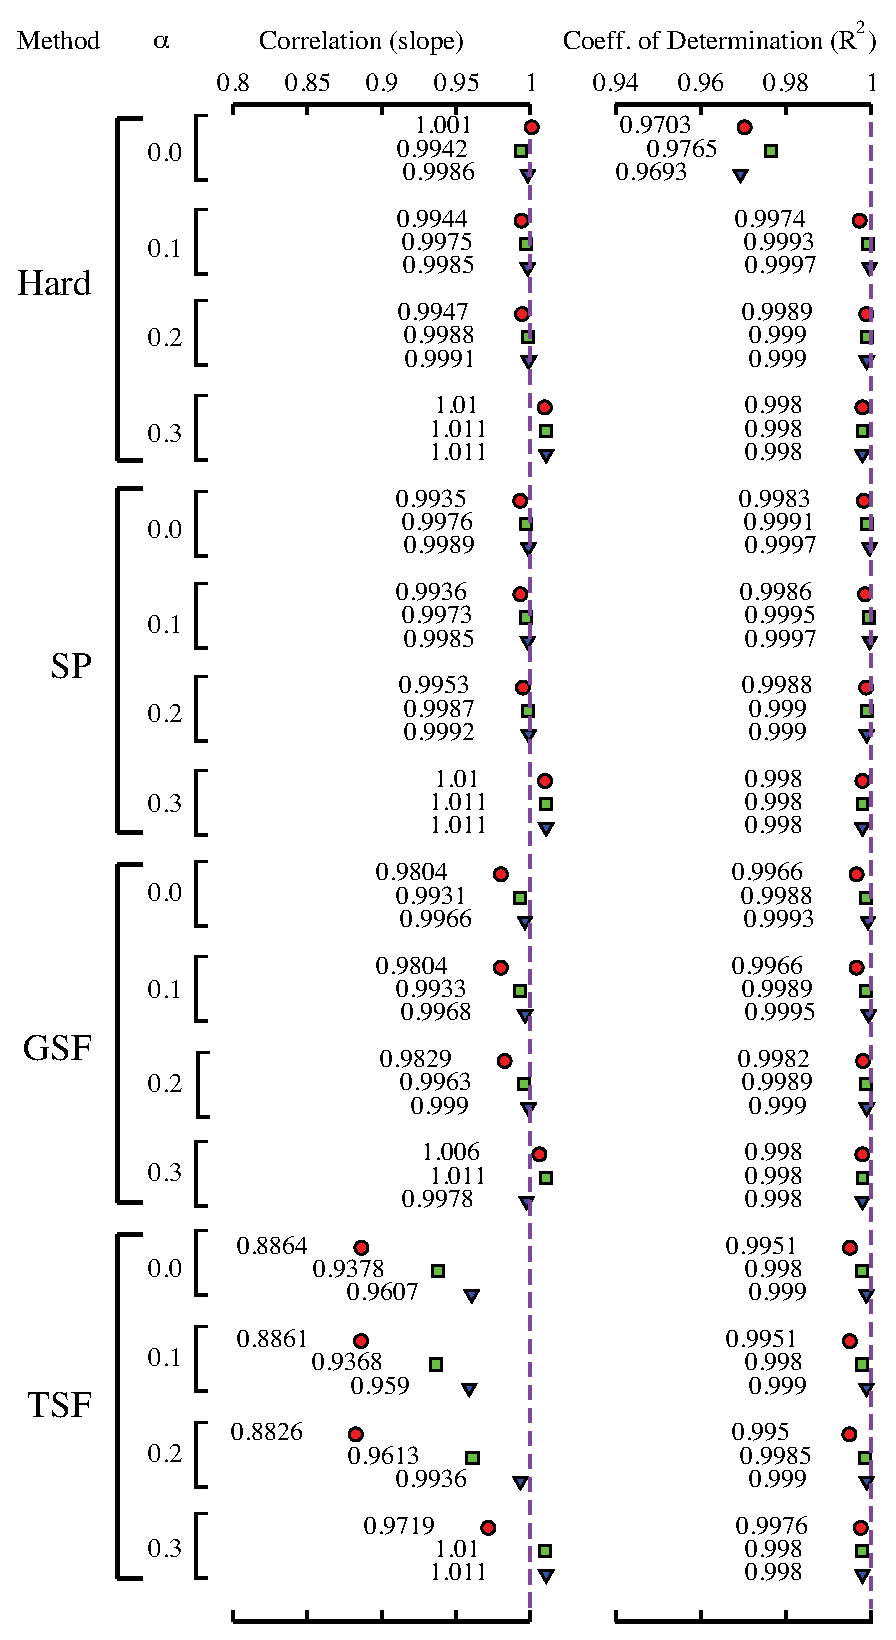
\includegraphics[width=0.6\linewidth]{energyPlot_slopeCorrelation_combined.eps}
  \caption{Statistical analysis of the quality of configurational
    energy differences for the real-space electrostatic methods
    compared with the reference Ewald sum.  Results with a value equal
    to 1 (dashed line) indicate $\Delta E$ values indistinguishable
    from those obtained using the multipolar Ewald sum.  Different
    values of the cutoff radius are indicated with different symbols
    (9~\AA\ = circles, 12~\AA\ = squares, and 15~\AA\ = inverted
    triangles).\label{fig:slopeCorr_energy}}
\end{figure} 

The combined coefficient of determination and slope for all six
systems is shown in Fig.~\ref{fig:slopeCorr_energy}.  Most of the
methods reproduce the Ewald configurational energy differences with
remarkable fidelity.  Undamped hard cutoffs introduce a significant
amount of random scatter in the energy differences which is apparent
in the reduced value of $R^2$ for this method.  This can be easily
understood as configurations which exhibit small traversals of a few
dipoles or quadrupoles out of the cutoff sphere will see large energy
jumps when hard cutoffs are used.  The orientations of the multipoles
(particularly in the ordered crystals) mean that these energy jumps
can go in either direction, producing a significant amount of random
scatter, but no systematic error.

The TSF method produces energy differences that are highly correlated
with the Ewald results, but it also introduces a significant
systematic bias in the values of the energies, particularly for
smaller cutoff values. The TSF method alters the distance dependence
of different orientational contributions to the energy in a
non-uniform way, so the size of the cutoff sphere can have a large
effect, particularly for the crystalline systems.

Both the SP and GSF methods appear to reproduce the Ewald results with
excellent fidelity, particularly for moderate damping ($\alpha \approx
0.2$~\AA$^{-1}$) and with a commonly-used cutoff value ($r_c =
12$~\AA).  With the exception of the undamped hard cutoff, and the TSF
method with short cutoffs, all of the methods would be appropriate for
use in Monte Carlo simulations.
\subsection{Magnitude of the force and torque vectors}

The comparisons of the magnitudes of the forces and torques for the
data accumulated from all six systems are shown in Fig.
~\ref{fig:slopeCorr_force} and \ref{fig:slopeCorr_torque}. The
correlation and slope for the forces agree well with the Ewald sum
even for the hard cutoffs.

For systems of molecules with only multipolar interactions, the pair
energy contributions are quite short ranged.  Moreover, the force
decays more rapidly than the electrostatic energy, hence the hard
cutoff method can also produce reasonable agreement for this quantity.
Although the pure cutoff gives reasonably good electrostatic forces
for pairs of molecules included within each other's cutoff spheres,
the discontinuity in the force at the cutoff radius can potentially
cause energy conservation problems as molecules enter and leave the
cutoff spheres.  This is discussed in detail in section
\ref{sec:conservation}.

The two shifted-force methods (GSF and TSF) exhibit a small amount of
systematic variation and scatter compared with the Ewald forces.  The
shifted-force models intentionally perturb the forces between pairs of
molecules inside each other's cutoff spheres in order to correct the
energy conservation issues, and this perturbation is evident in the
statistics accumulated for the molecular forces.  The GSF
perturbations are minimal, particularly for moderate damping and
commonly-used cutoff values ($r_c = 12$~\AA).  The TSF method shows
reasonable agreement in $R^2$, but again the systematic error in the
forces is concerning if replication of Ewald forces is desired.

It is important to note that the forces and torques from the SP and
the Hard cutoffs are not identical. The SP method shifts each
orientational contribution separately (e.g. the dipole-dipole dot
product is shifted by a different function than the dipole-distance
products), while the hard cutoff contains no orientation-dependent
shifting.  The forces and torques for these methods therefore diverge
for multipoles even though the forces for point charges are identical.

\begin{figure}
  \centering
  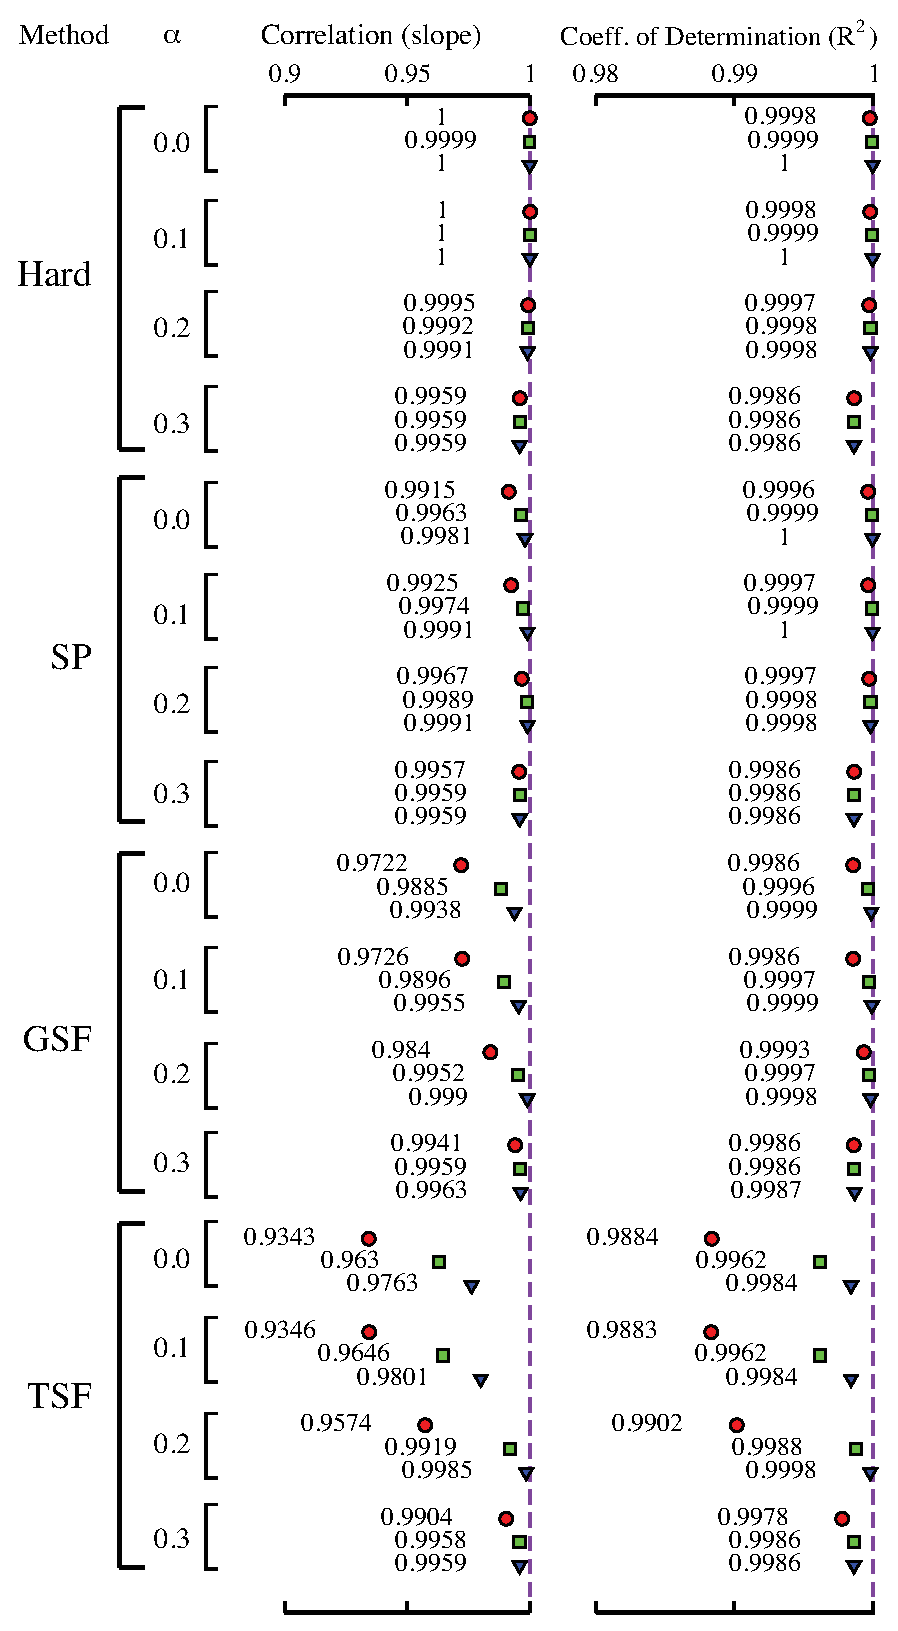
\includegraphics[width=0.6\linewidth]{forcePlot_slopeCorrelation_combined.eps} 
  \caption{Statistical analysis of the quality of the force vector
    magnitudes for the real-space electrostatic methods compared with
    the reference Ewald sum. Results with a value equal to 1 (dashed
    line) indicate force magnitude values indistinguishable from those
    obtained using the multipolar Ewald sum.  Different values of the
    cutoff radius are indicated with different symbols (9~\AA\ =
    circles, 12~\AA\ = squares, and 15~\AA\ = inverted
    triangles).\label{fig:slopeCorr_force}}
\end{figure} 


\begin{figure}
  \centering
  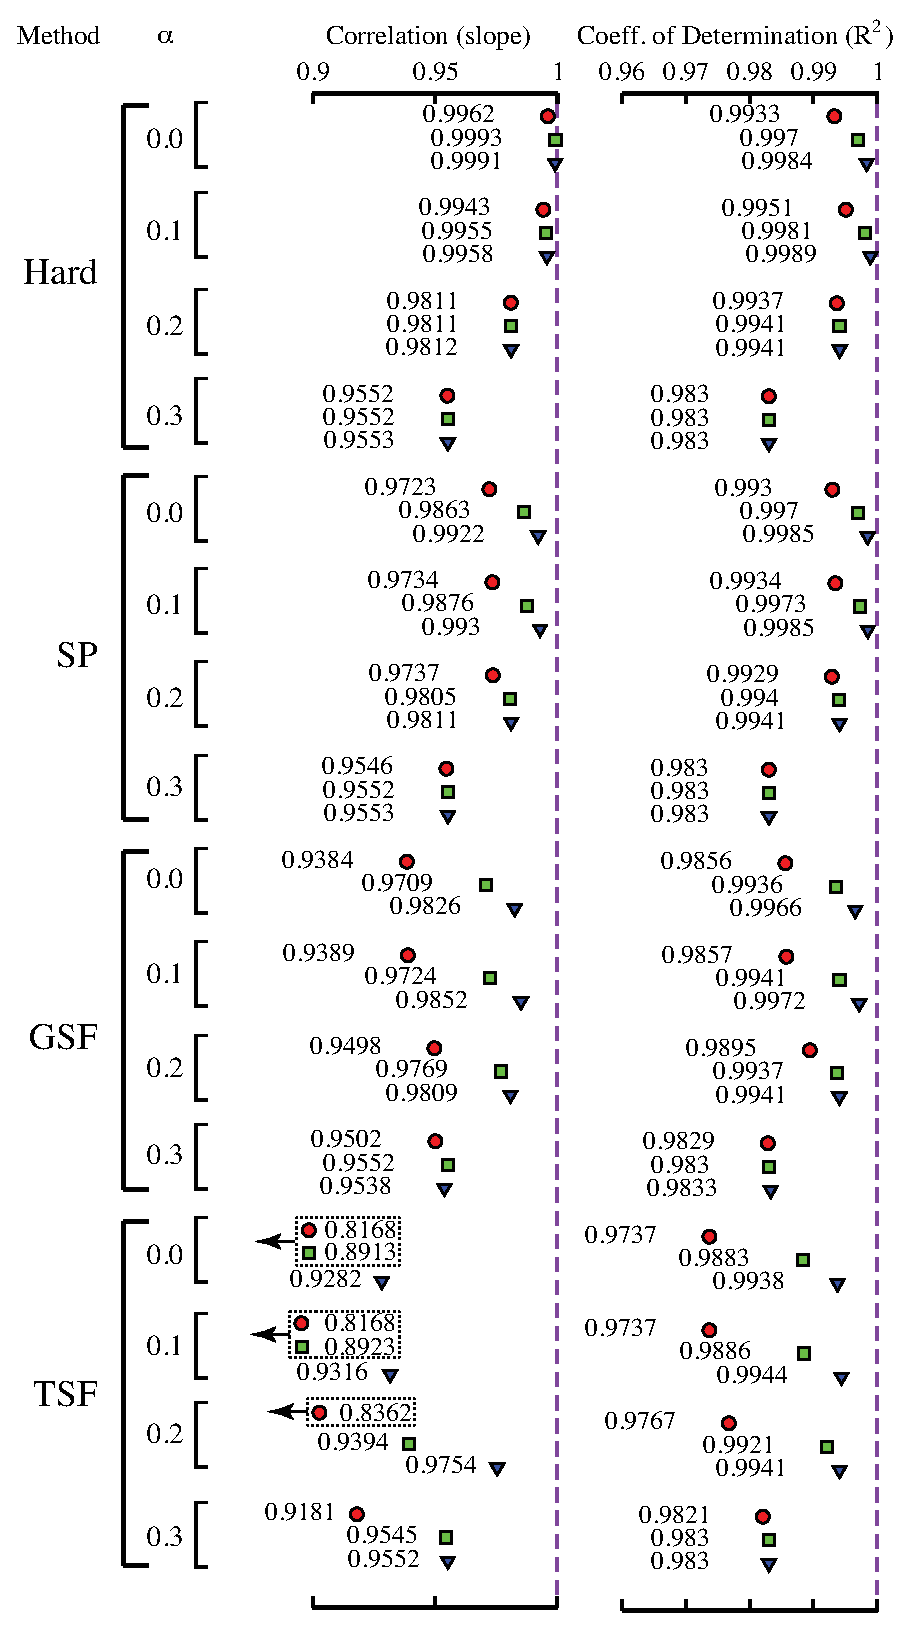
\includegraphics[width=0.6\linewidth]{torquePlot_slopeCorrelation_combined.eps}
  \caption{Statistical analysis of the quality of the torque vector
    magnitudes for the real-space electrostatic methods compared with
    the reference Ewald sum. Results with a value equal to 1 (dashed
    line) indicate force magnitude values indistinguishable from those
    obtained using the multipolar Ewald sum.  Different values of the
    cutoff radius are indicated with different symbols (9~\AA\ =
    circles, 12~\AA\ = squares, and 15~\AA\ = inverted
    triangles).\label{fig:slopeCorr_torque}}
\end{figure}

The torques (Fig. \ref{fig:slopeCorr_torque}) appear to be
significantly influenced by the choice of real-space method.  The
torque expressions have the same distance dependence as the energies,
which are naturally longer-ranged expressions than the inter-site
forces.  Torques are also quite sensitive to orientations of
neighboring molecules, even those that are near the cutoff distance.

The results shows that the torque from the hard cutoff method
reproduces the torques in quite good agreement with the Ewald sum.
The other real-space methods can cause some deviations, but excellent
agreement with the Ewald sum torques is recovered at moderate values
of the damping coefficient ($\alpha \approx 0.2$~\AA$^{-1}$) and cutoff
radius ($r_c \ge 12$~\AA).  The TSF method exhibits only fair agreement
in the slope when compared with the Ewald torques even for larger
cutoff radii.  It appears that the severity of the perturbations in
the TSF method are most in evidence for the torques.

\subsection{Directionality of the force and torque vectors}   

The accurate evaluation of force and torque directions is just as
important for molecular dynamics simulations as the magnitudes of
these quantities. Force and torque vectors for all six systems were
analyzed using Fisher statistics, and the quality of the vector
directionality is shown in terms of circular variance
($\mathrm{Var}(\theta)$) in
Fig. \ref{fig:slopeCorr_circularVariance}. The force and torque
vectors from the new real-space methods exhibit nearly-ideal Fisher
probability distributions (Eq.~\ref{eq:pdf}). Both the hard and SP
cutoff methods exhibit the best vectorial agreement with the Ewald
sum. The force and torque vectors from GSF method also show good
agreement with the Ewald method, which can also be systematically
improved by using moderate damping and a reasonable cutoff radius. For
$\alpha = 0.2$~\AA$^{-1}$ and $r_c = 12$~\AA, we observe
$\mathrm{Var}(\theta) = 0.00206$, which corresponds to a distribution
with 95\% of force vectors within $6.37^\circ$ of the corresponding
Ewald forces. The TSF method produces the poorest agreement with the
Ewald force directions.

Torques are again more perturbed than the forces by the new real-space
methods, but even here the variance is reasonably small.  For the same
method (GSF) with the same parameters ($\alpha = 0.2$~\AA$^{-1}$, $r_c
= 12$~\AA), the circular variance was 0.01415, corresponds to a
distribution which has 95\% of torque vectors are within $16.75^\circ$
of the Ewald results. Again, the direction of the force and torque
vectors can be systematically improved by varying $\alpha$ and $r_c$.

\begin{figure}
  \centering
  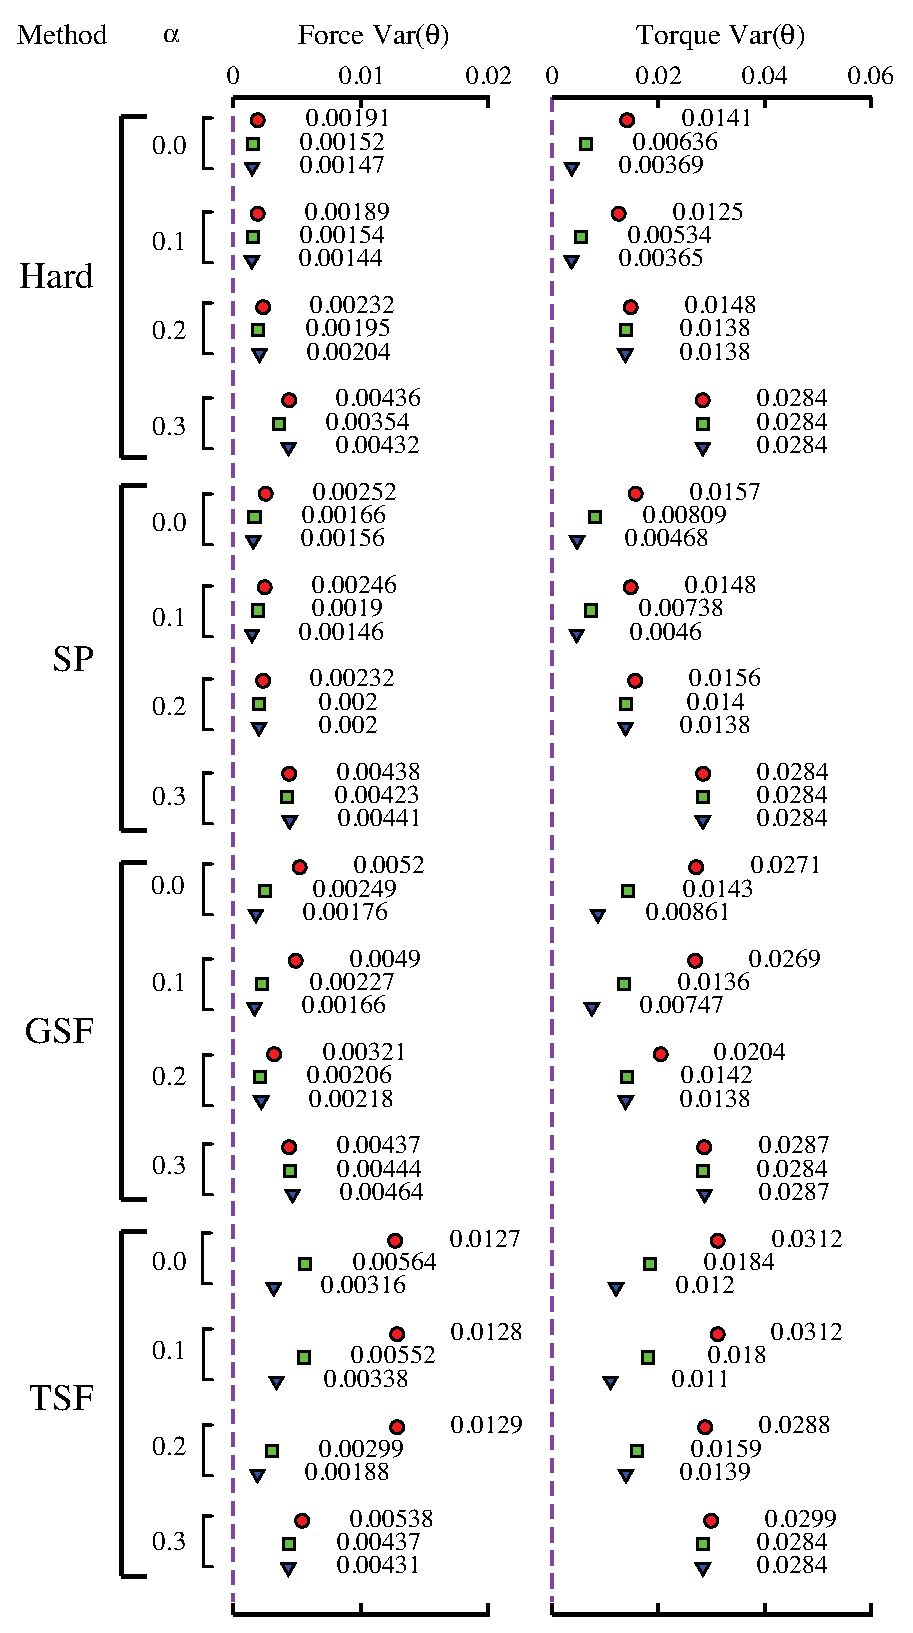
\includegraphics[width=0.65\linewidth]{Variance_forceNtorque_modified.eps}
  \caption{The circular variance of the direction of the force and
    torque vectors obtained from the real-space methods around the
    reference Ewald vectors. A variance equal to 0 (dashed line)
    indicates direction of the force or torque vectors are
    indistinguishable from those obtained from the Ewald sum. Here
    different symbols represent different values of the cutoff radius
    (9~\AA\ = circle, 12~\AA\ = square, 15~\AA\ = inverted triangle)\label{fig:slopeCorr_circularVariance}}
\end{figure}

\subsection{Energy conservation\label{sec:conservation}}

We have tested the conservation of energy one can expect to see with
the new real-space methods using the soft DQ liquid model with a small
fraction of solvated ions. This is a test system which exercises all
orders of multipole-multipole interactions derived in the chapter 2
in this series and provides the most comprehensive test of the new
methods.  A liquid-phase system was created with 2000 liquid-phase
molecules and 48 dissolved ions at a density of 0.98 g cm$^{-3}$ and a
temperature of 300K.  After equilibration in the canonical (NVT)
ensemble using a Nos\'e-Hoover thermostat, six
statistically-independent replicas of this liquid-phase system were
run in the microcanonical (NVE) ensemble under the Ewald, Hard, SP,
GSF, and TSF methods with a cutoff radius of 12~\AA.  The value of the
damping coefficient was also varied from the undamped case ($\alpha =
0$) to a heavily damped case ($\alpha = 0.3$~\AA$^{-1}$) for all of
the real space methods.  A sample was also run using the multipolar
Ewald sum with the same real-space cutoff.

In Fig.~\ref{fig:energyDrift} we show the both the linear drift in
energy over time, $\delta E_1$, and the standard deviation of energy
fluctuations around this drift $\delta E_0$.  Both of the
shifted-force methods (GSF and TSF) provide excellent energy
conservation (drift less than $10^{-5}$ kcal / mol / ns / particle),
while the hard cutoff is essentially unusable for molecular dynamics.
SP provides some benefit over the hard cutoff because the energetic
jumps that happen as particles leave and enter the cutoff sphere are
somewhat reduced, but like the Wolf method for charges, the SP method
would not be as useful for molecular dynamics as either of the
shifted-force methods.

We note that for all tested values of the cutoff radius, the new
real-space methods can provide better energy conservation behavior
than the multipolar Ewald sum, even when relatively large $k$-space
cutoff values are utilized.

\begin{figure}
  \centering
  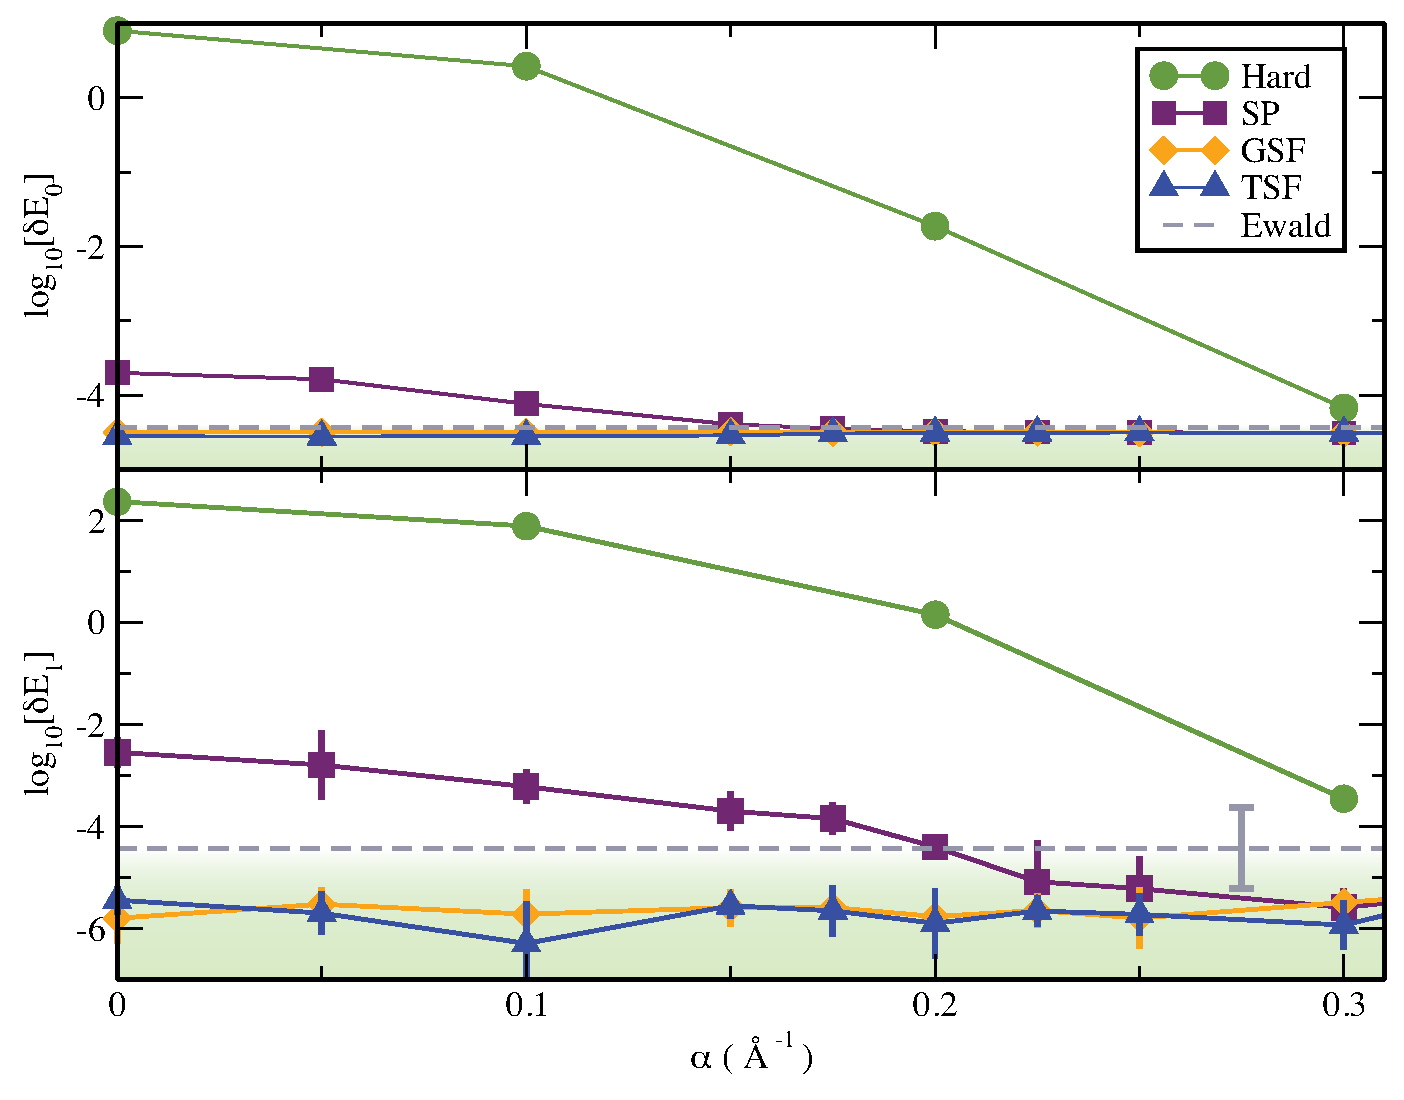
\includegraphics[width=\textwidth]{finalDrift.eps}
  \caption{Energy conservation of the real-space methods for the soft
    DQ liquid / ion system. $\delta \mathrm{E}_1$ is the linear drift
    in energy over time (in kcal/mol/particle/ns) and $\delta
    \mathrm{E}_0$ is the standard deviation of energy fluctuations
    around this drift (in kcal/mol/particle).  Points that appear in
    the green region at the bottom exhibit better energy conservation
    than would be obtained using common parameters for Ewald-based
    electrostatics.\label{fig:energyDrift}}
\end{figure} 
\subsection{Reproduction of Structural \& Dynamical Features\label{sec:structure}}
The most important test of the modified interaction potentials is the
fidelity with which they can reproduce structural features and
dynamical properties in a liquid.  One commonly-utilized measure of
structural ordering is the pair distribution function, $g(r)$, which
measures local density deviations in relation to the bulk density.  In
the electrostatic approaches studied here, the short-range repulsion
from the Lennard-Jones potential is identical for the various
electrostatic methods, and since short range repulsion determines much
of the local liquid ordering, one would not expect to see many
differences in $g(r)$.  Indeed, the pair distributions are essentially
identical for all of the electrostatic methods studied (for each of
the different systems under investigation). 

% An example of this agreement for the soft DQ liquid/ion system is
% shown in Fig. \ref{fig:gofr}.

% \begin{figure}
%   \centering
%   \includegraphics[width=\textwidth]{gofr_ssdqc.eps}
% \caption{The pair distribution functions, $g(r)$, for the SSDQ
%   water/ion system obtained using the different real-space methods are
%   essentially identical with the result from the Ewald
%   treatment.\label{fig:gofr}}
% \end{figure} 

There is a minor over-structuring of the first solvation shell when
using TSF or when overdamping with any of the real-space methods.
With moderate damping, GSF and SP produce pair distributions that are
identical (within numerical noise) to their Ewald counterparts.  The
degree of over-structuring can be measured most easily using the
coordination number,
\begin{equation}
n_C = 4\pi\rho \int_{0}^{a}r^2\text{g}(r)dr,
\end{equation}
where $\rho$ is the number density of the site-site pair interactions,
and $a$ is the radial location of the minima following the first peak
in $g(r)$ ($a = 4.2$~\AA\  for the soft DQ liquid / ion system).  The
coordination number is shown as a function of the damping coefficient
for all of the real space methods in Fig. \ref{fig:Props}.

A more demanding test of modified electrostatics is the average value
of the electrostatic energy $\langle U_\mathrm{elect} \rangle / N$
which is obtained by sampling the liquid-state configurations
experienced by a liquid evolving entirely under the influence of each
of the methods.  In Fig. \ref{fig:Props} we demonstrate how $\langle
U_\mathrm{elect} \rangle / N$ varies with the damping parameter,
$\alpha$, for each of the methods. 

As in the crystals studied in the chapter 2, damping is important
for converging the mean electrostatic energy values, particularly for
the two shifted force methods (GSF and TSF).  A value of $\alpha
\approx 0.2$~\AA$^{-1}$ is sufficient to converge the SP and GSF
energies with a cutoff of 12 \AA, while shorter cutoffs require more
dramatic damping ($\alpha \approx 0.28$~\AA$^{-1}$ for $r_c = 9$~\AA).
Overdamping the real-space electrostatic methods occurs with $\alpha >
0.3$~\AA$^{-1}$, causing the estimate of the electrostatic energy to
drop below the Ewald results.

These ``optimal'' values of the damping coefficient for structural
features are similar to those observed for DSF electrostatics for
purely point-charge systems, and the range $\alpha= 0.175 \rightarrow
0.225$~\AA$^{-1}$ for $r_c = 12$~\AA\ appears to be an excellent
compromise for mixed charge/multipolar systems.

To test the fidelity of the electrostatic methods at reproducing
\textit{dynamics} in a multipolar liquid, it is also useful to look at
transport properties, particularly the diffusion constant,
\begin{equation}
D = \lim_{t \rightarrow \infty} \frac{1}{6 t} \langle \left|
  \mathbf{r}(t) -\mathbf{r}(0) \right|^2 \rangle
\label{eq:diff}
\end{equation}
which measures long-time behavior and is sensitive to the forces on
the multipoles. The self-diffusion constants (D) were calculated from
linear fits to the long-time portion of the mean square displacement,
$\langle r^{2}(t) \rangle$.\cite{Allen89} In Fig. \ref{fig:Props} we
demonstrate how the diffusion constant depends on the choice of
real-space methods and the damping coefficient.  Both the SP and GSF
methods can obtain excellent agreement with Ewald again using moderate
damping.

In addition to translational diffusion, orientational relaxation times
were calculated for comparisons with the Ewald simulations and with
experiments. These values were determined by calculating the
orientational time correlation function,
\begin{equation}
C_l^\gamma(t) = \left\langle P_l\left[\hat{\mathbf{A}}_\gamma(t)
                \cdot\hat{\mathbf{A}}_\gamma(0)\right]\right\rangle,
\label{eq:OrientCorr}
\end{equation}
from the same 350 ps microcanonical trajectories that were used for
translational diffusion.  Here, $P_l$ is the Legendre polynomial of
order $l$ and $\hat{\mathbf{A}}_\gamma$ is the unit vector for body
axis $\gamma$.  The reference frame used for our sample dipolar
systems has the $z$-axis running along the dipoles, and for the soft
DQ liquid model, the $y$-axis connects the two implied hydrogen-like
positions.  From the orientation autocorrelation functions, we can
obtain time constants for rotational relaxation either by fitting to a
multi-exponential model for the orientational relaxation, or by
integrating the correlation functions.

In a good model for water, the orientational decay times would be
comparable to water orientational relaxation times from nuclear
magnetic resonance (NMR). The relaxation constant obtained from
$C_2^y(t)$ is normally of experimental interest because it describes
the relaxation of the principle axis connecting the hydrogen
atoms. Thus, $C_2^y(t)$ can be compared to the intermolecular portion
of the dipole-dipole relaxation from a proton NMR signal and can
provide an estimate of the NMR relaxation time constant.\cite{Impey82}
In Fig. \ref{fig:Props} we compare the $\tau_2^y$ and $\tau_2^z$
values for the various real-space methods over a range of different
damping coefficients.  The rotational relaxation for the $z$ axis
primarily probes the torques on the dipoles, while the relaxation for
the $y$ axis is sensitive primarily to the quadrupolar torques.

\begin{figure}
  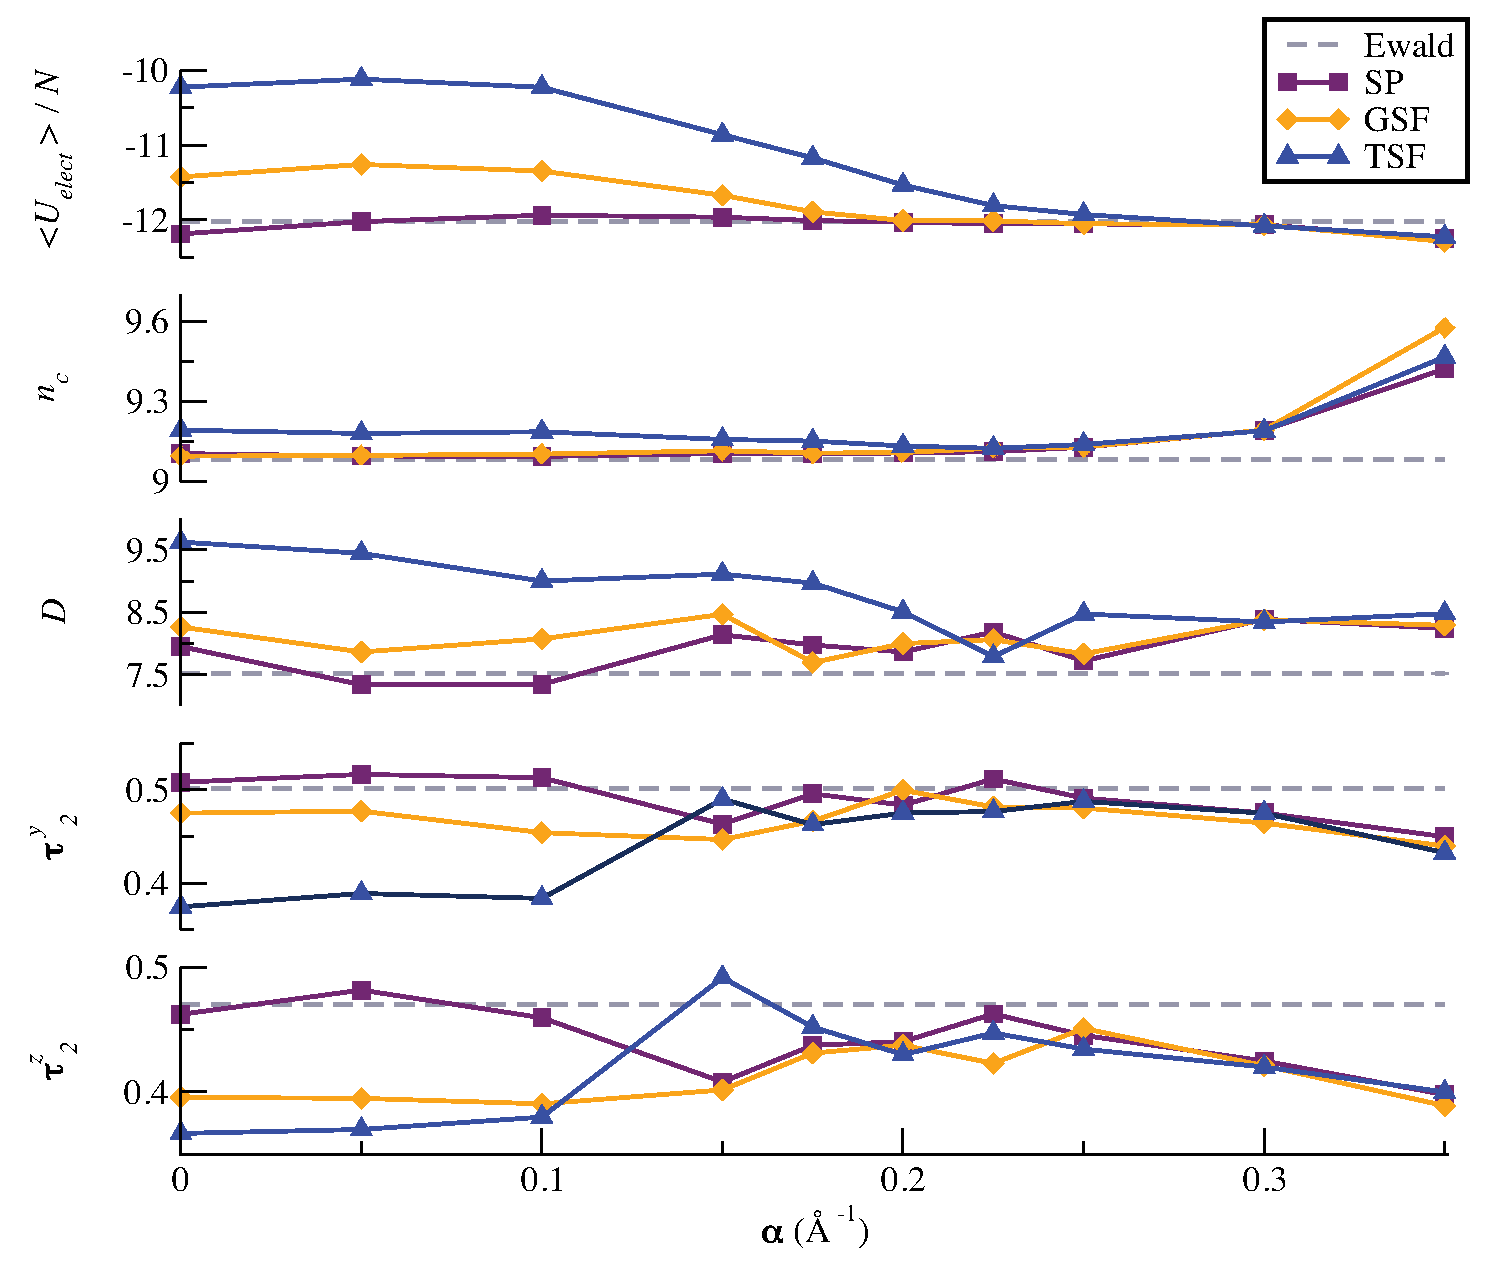
\includegraphics[width=\textwidth]{properties.eps}
  \caption{Comparison of the structural and dynamic properties for the
    combined multipolar liquid (soft DQ liquid + ions) for all of the
    real-space methods with $r_c = 12$~\AA. Electrostatic energies,
    $\langle U_\mathrm{elect} \rangle / N$ (in kcal / mol),
    coordination numbers, $n_C$, diffusion constants (in $10^{-5}
    \mathrm{cm}^2\mathrm{s}^{-1}$), and rotational correlation times
    (in ps) all show excellent agreement with Ewald results for
    damping coefficients in the range $\alpha= 0.175 \rightarrow
    0.225$~\AA$^{-1}$. \label{fig:Props}}
\end{figure}

In Fig. \ref{fig:Props} it appears that values for $D$, $\tau_2^y$,
and $\tau_2^z$ using the Ewald sum are reproduced with excellent
fidelity by the GSF and SP methods.  All of the real space methods can
be \textit{overdamped}, which reduces the effective range of multipole
interactions, causing structural and dynamical changes from the
correct behavior.  Because overdamping weakens orientational
preferences between adjacent molecules, it manifests as too-rapid
orientational decay coupled with faster diffusion and
over-coordination of the liquid.  Underdamping is less problematic for
the SP and GSF methods, as their structural and dynamical properties
still reproduce the Ewald results even in the completely undamped
($\alpha = 0$) case.  An optimal range for the electrostatic damping
parameter appears to be $\alpha= 0.175 \rightarrow 0.225$~\AA$^{-1}$
for $r_c = 12$~\AA, which similar to the optimal range found for the
damped shifted force potential for point charges.\cite{Gezelter06}

\section{Summary}
In the chapter 2, we generalized the
charge-neutralized electrostatic energy originally developed by Wolf
\textit{et al.}\cite{Wolf99} to multipole-multipole interactions
up to quadrupolar order.  The SP method is essentially a
multipole-capable version of the Wolf model.  The SP method for
multipoles provides excellent agreement with Ewald-derived energies,
forces and torques, and is suitable for Monte Carlo simulations,
although the forces and torques retain discontinuities at the cutoff
distance that prevents its use in molecular dynamics.

We also developed two natural extensions of the damped shifted-force
(DSF) model originally proposed by Zahn {\it et al.} and extended by
Fennell and Gezelter.\cite{Zahn02, Gezelter06} The GSF and TSF
approaches provide smooth truncation of energies, forces, and torques
at the real-space cutoff, and both converge to DSF electrostatics for
point-charge interactions.  The TSF model is based on a high-order
truncated Taylor expansion which can be relatively perturbative inside
the cutoff sphere.  The GSF model takes the gradient from an images of
the interacting multipole that has been projected onto the cutoff
sphere to derive shifted force and torque expressions, and is a
significantly more gentle approach.

The GSF method produces quantitative agreement with Ewald energies,
forces, and torques.  It also performs well in conserving energy in MD
simulations.  The Taylor-shifted (TSF) model provides smooth dynamics,
but these take place on a potential energy surface that is
significantly perturbed from Ewald-based electrostatics.  Because it
performs relatively poorly compared with GSF, it may seem odd that
that the TSF model was included in this work.  However, the functional
forms derived for the SP and GSF methods depend on the separation of
orientational contributions that were made visible by the Taylor
series of the electrostatic kernel at the cutoff radius. The TSF
method also has the unique property that a large number of derivatives
can be made to vanish at the cutoff radius.  This property has proven
useful in past treatments of the corrections to the Clausius-Mossotti
fluctuation formula for dielectric constants.\cite{Izvekov08}

Reproduction of both structural and dynamical features in the liquid
systems is remarkably good for both the SP and GSF models.  Pair
distribution functions are essentially equivalent to the same
functions produced using Ewald-based electrostatics, and with moderate
damping, a structural feature that directly probes the electrostatic
interaction (e.g. the mean electrostatic potential energy) can also be
made quantitative.  Dynamical features are sensitive probes of the
forces and torques produced by these methods, and even though the
smooth behavior of forces is produced by perturbing the overall
potential, the diffusion constants and orientational correlation times
are quite close to the Ewald-based results.

The only cases we have found where the new GSF and SP real-space
methods can be problematic are those which retain a bulk dipole moment
at large distances (e.g. the $Z_1$ dipolar lattice).  In ferroelectric
materials, uniform weighting of the orientational contributions can be
important for converging the total energy.  In these cases, the
damping function which causes the non-uniform weighting can be
replaced by the bare electrostatic kernel, and the energies return to
the expected converged values.

Based on the results of this work, we can conclude that the GSF method
is a suitable and efficient replacement for the Ewald sum for
evaluating electrostatic interactions in modern MD simulations, and
the SP method would be an excellent choice for Monte Carlo
simulations where smooth forces and energy conservation are not
important.  Both the SP and GSF methods retain excellent fidelity to
the Ewald energies, forces and torques.  Additionally, the energy
drift and fluctuations from the GSF electrostatics are significantly
better than a multipolar Ewald sum for finite-sized reciprocal spaces,
and physical properties are reproduced accurately.

As in all purely pairwise cutoff methods, the SP, GSF and TSF methods
are expected to scale approximately {\it linearly} with system size,
and are easily parallelizable.  This should result in substantial
reductions in the computational cost of performing large simulations.
With the proper use of pre-computation and spline interpolation of the
radial functions, the real-space methods are essentially the same cost
as a simple real-space cutoff.  They require no Fourier transforms or
$k$-space sums, and guarantee the smooth handling of energies, forces,
and torques as multipoles cross the real-space cutoff boundary.

We are not suggesting that there is any flaw with the Ewald sum; in
fact, it is the standard by which the SP, GSF, and TSF methods have
been judged in this work.  However, these results provide evidence
that in the typical simulations performed today, the Ewald summation
may no longer be required to obtain the level of accuracy most
researchers have come to expect.



% % uncomment the following lines,
% if using chapter-wise bibliography
%
% \bibliographystyle{ndnatbib}
% \bibliography{example}


% Chapter 4

%
% Modified by Megan Patnott
% Last Change: Jan 18, 2013
%
%%%%%%%%%%%%%%%%%%%%%%%%%%%%%%%%%%%%%%%%%%%%%%%%%%%%%%%%%%%%%%%%%%%%%%%%
%
% Modified by Sameer Vijay
% Last Change: Wed Jul 27 2005 13:00 CEST
%
%%%%%%%%%%%%%%%%%%%%%%%%%%%%%%%%%%%%%%%%%%%%%%%%%%%%%%%%%%%%%%%%%%%%%%%%
%
% Sample Notre Dame Thesis/Dissertation
% Using Donald Peterson's ndthesis classfile
%
% Written by Jeff Squyres and Don Peterson
%
% Provided by the Information Technology Committee of
%   the Graduate Student Union
%   http://www.gsu.nd.edu/
%
% Nothing in this document is serious except the format.  :-)
%
% If you have any suggestions, comments, questions, please send e-mail
% to: ndthesis@gsu.nd.edu
%
%%%%%%%%%%%%%%%%%%%%%%%%%%%%%%%%%%%%%%%%%%%%%%%%%%%%%%%%%%%%%%%%%%%%%%%%

%
% Chapter 4
%

\chapter{DIELECTRIC PROPERTIES}
\label{chap:dielectric}
In the chapter 3, I have presented various physical properties calculated using SP, GSF,TSF, and Ewald methods. This chapter reports on the fluctuation, perturbation, and potential of mean force (PMF) methods for calculating dielectric properties for dipolar and quadrupolar fluids. Since the dielectric constant is a macroscopic property, interactions of a molecule with the all of the molecules in the system should be considered. But the real space methods utilize a cutoff radius and ignores the interaction beyond cutoff radius. Hence the formula for calculating dielectric constant should be modified accordingly. To evaluate correct dielectric properties from the simulation, we have to take account of correction factor for each real-space methods. In this chapter, I have also presented the correction factor required for the calculation of the dielectric properties for dipolar and quadrupolar fluids.

\section{Introduction}

One of the most stringent tests of any new electrostatic method is the
fidelity with which that method can reproduce the bulk-phase
polarizability or equivalently, the dielectric properties of a
fluid. Before the advent of computer simulations, Kirkwood and Onsager
developed fluctuation formulae for the dielectric properties of
dipolar fluids.\cite{Kirkwood39,Onsagar36} Along with projections of
the frequency-dependent dielectric to zero frequency, these
fluctuation formulae are now widely used to predict the static
dielectric constant of simulated materials.

If we consider a system of dipolar or quadrupolar molecules under the
influence of an external field or field gradient, the net polarization
of the system will largely be proportional to the applied
perturbation.\cite{Chitanvis96, Stern-Feller03, SalvchovI14,SalvchovII14} In simulations, the net polarization of the system is
also determined by the interactions \textit{between} the
molecules. Therefore the macroscopic polarizablity obtained from a
simulation depends on the details of the electrostatic interaction
methods that were employed in the simulation. To determine the
relevant physical properties of the multipolar fluid from the system
fluctuations, the interactions between molecules must be incorporated
into the formalism for the bulk properties.

In most simulations, bulk materials are treated using periodic
replicas of small regions, and this level of approximation requires
corrections to the fluctuation formulae that were derived for the bulk
fluids. In 1983 Neumann proposed a general formula for evaluating
dielectric properties of dipolar fluids using both Ewald and
real-space cutoff methods.\cite{NeumannI83} Steinhauser and Neumann
used this formula to evaluate the corrected dielectric constant for
the Stockmayer fluid using two different methods: Ewald-Kornfeld (EK)
and reaction field (RF) methods.\cite{NeumannII83}

Zahn \textit{et al.}\cite{Zahn02} utilized this approach and evaluated
the correction factor for using damped shifted charge-charge
kernel. This was later generalized by Izvekov \textit{et
  al.},\cite{Izvekov08} who noted that the expression for the
dielectric constant reduces to widely-used conducting boundary formula
for real-space methods that have first derivatives that vanish at the
cutoff radius.

One of the primary topics of this chapter is the derivation of
correction factors for the three new real space methods.  We find that
the correction formulae for dipolar molecules depends not only on the
methodology being used, but also on whether the molecular dipoles are
treated using point charges or point dipoles.  We derive correction
factors for both cases.

In quadrupolar fluids, the relationship between quadrupolar
susceptibility and the dielectric constant is not as straightforward
as in the dipolar case.  The effective dielectric constant depends on
the geometry of the external (or internal) field
perturbation.\cite{Ernst92} Significant efforts have been made to
increase our understanding the dielectric properties of these
fluids,\cite{JeonI03,JeonII03,Chitanvis96} although a general
correction formula has not yet been developed.

In this chapter, we derive general formulae for calculating the
quadrupolar susceptibility of quadrupolar fluids. We also evaluate the
correction factor for SP, GSF, and TSF methods for quadrupolar fluids
interacting via point charges, point dipoles or directly through
quadrupole-quadrupole interactions.

We also calculate the screening behavior for two ions immersed in
multipolar fluids to estimate the distance dependence of charge
screening in both dipolar and quadrupolar fluids.  We use three
distinct methods to compare our analytical results with computer
simulations:
\begin{enumerate}
\item responses of the fluid to external perturbations,
\item fluctuations of system multipole moments, and
\item potentials of mean force between solvated ions,
\end{enumerate}

\begin{figure}
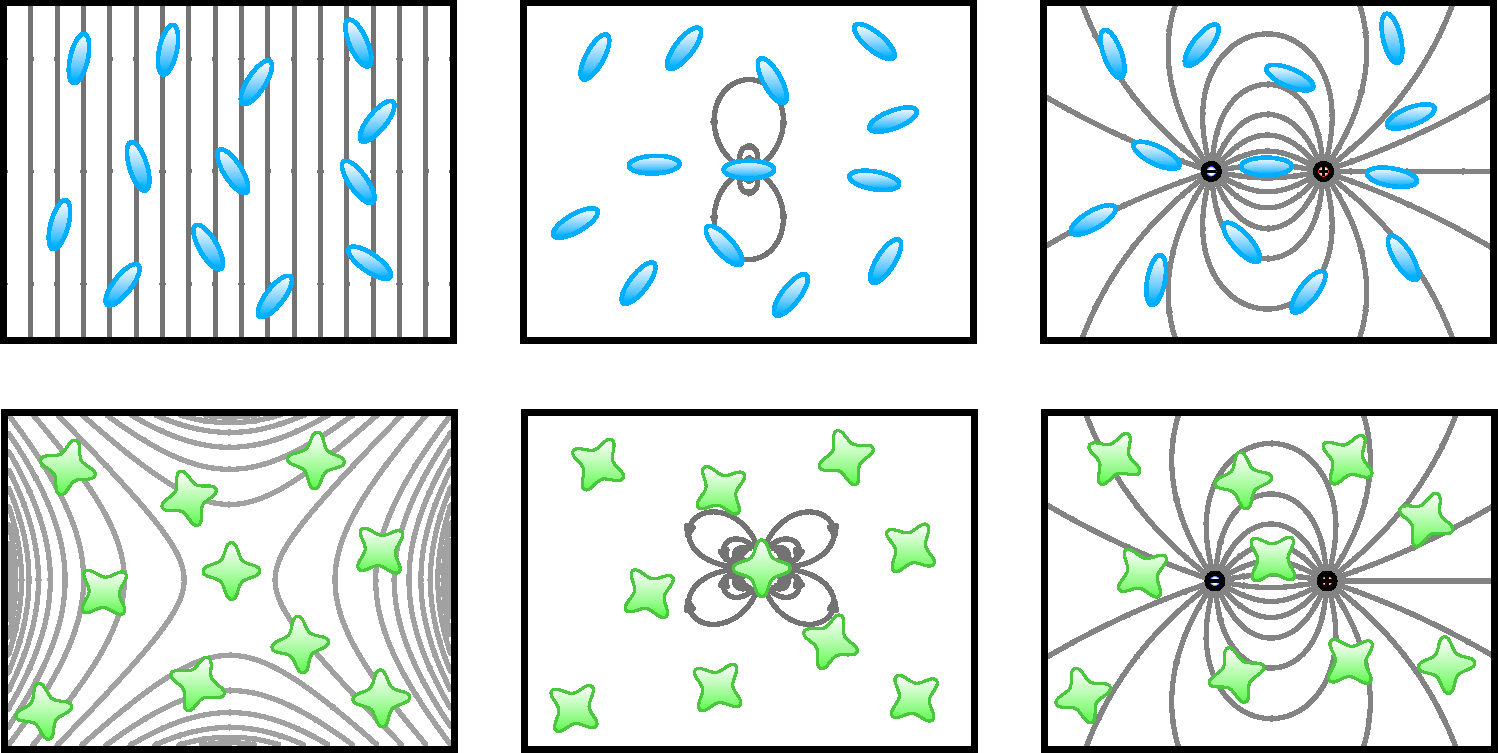
\includegraphics[width=\linewidth]{Schematic}
\caption{Dielectric properties of a fluid measure the response to
  external electric fields and gradients (left), or internal fields
  and gradients generated by the molecules themselves (center), or
  fields produced by embedded ions (right). The dielectric constant
  ($\epsilon$) measures all three responses in dipolar fluids (top).
  In quadrupolar liquids (bottom), the relevant bulk property is the
  quadrupolar susceptibility ($\chi_Q$), and the geometry of the field
  determines the effective dielectric screening.}
\label{fig:schematic}
\end{figure}

Under the influence of weak external fields, the bulk polarization of
the system is primarily a linear response to the perturbation, where
proportionality constant depends on the electrostatic interactions
between the multipoles. The fluctuation formulae connect bulk
properties of the fluid to equilibrium fluctuations in the system
multipolar moments during a simulation. These fluctuations also depend
on the form of the electrostatic interactions between molecules.
Therefore, the connections between the actual bulk properties and both
the computed fluctuation and external field responses must be modified
accordingly.

The potential of mean force (PMF) allows calculation of an effective
dielectric constant or screening factor from the potential energy
between ions before and after dielectric material is introduced.
Computing the PMF between embedded point charges is an additional
check on the bulk properties computed via the other two methods.

\section{Dipolar Fluids and the Dielectric Constant}

Dielectric properties of a fluid arise mainly from responses of the
fluid to either applied fields or transient fields internal to the
fluid. In response to an applied field, the molecules have electronic
polarizabilities, changes to internal bond lengths, and reorientations
towards the direction of the applied field. There is an added
complication that in the presence of external field, the perturbation
experienced by any single molecule is not only due to external field
but also to the fields produced by the all other molecules in the
system.

\subsection{Response to External Perturbations}

In the presence of uniform electric field $\mathbf{E}$, an individual
molecule with a permanent dipole moment $p_o$ will realign along the
direction of the field with an average polarization given by
\begin{equation}
\braket{\mathbf{p}} = \epsilon_0 \alpha_p \mathbf{E},
\end{equation}
where $\alpha_p = {p_o}^2 / 3 \epsilon_0 k_B T$ is the contribution to
molecular polarizability due solely to reorientation dynamics.
Because the applied field must overcome thermal motion, the
orientational polarization depends inversely on the temperature.

Likewise, a condensed phase system of permanent dipoles will also
polarize along the direction of an applied field. The polarization
density of the system is
\begin{equation}
\textbf{P} = \epsilon_o \alpha_{D} \mathbf{E}. 
\label{pertDipole}
\end{equation} 
The constant $\alpha_D$ is the macroscopic polarizability, which is an
emergent property of the dipolar fluid.  Note that the polarizability,
$\alpha_D$ is distinct from the dipole susceptibility, $\chi_D$,
which is the quantity most directly related to the static dielectric
constant, $\epsilon = 1 + \chi_D$.

\subsection{Fluctuation Formula}

For a system of dipolar molecules at thermal equilibrium, we can
define both a system dipole moment, $\mathbf{M} = \sum_i \mathbf{p}_i$
as well as a dipole polarization density,
$\mathbf{P} = \braket{\mathbf{M}}/V$.

In the presence of applied field $\mathbf{E}$, the polarization
density can be expressed in terms of fluctuations in the net dipole
moment,
\begin{equation}
\mathbf{P} = \epsilon_o \frac{\braket{\mathbf{M}^2}-{\braket{\mathbf{M}}}^2}{3 \epsilon_o V k_B T}\bf{E}
\label{flucDipole}
\end{equation}
This has structural similarity with the Boltzmann average for the
polarization of a single molecule. Here
$ \braket{\mathbf{M}^2}-{\braket{\mathbf{M}}}^2$ measures fluctuations
in the net dipole moment,
\begin{equation}
 \langle \mathbf{M}^2 \rangle - \langle \mathbf{M} \rangle^2 =
 \langle M_x^2+M_y^2+M_z^2 \rangle - \left( \langle M_x \rangle^2 +
   \langle M_y \rangle^2 +
   \langle M_z \rangle^2 \right).
\label{eq:flucDip}
\end{equation}
For the limiting case $\textbf{E} \rightarrow 0 $, the ensemble
average of both the net dipole moment $\braket{\mathbf{M}}$ and
dipolar polarization $\bf{P}$ tends to vanish but
$\braket{\mathbf{M}^2}$ does not.  The macroscopic dipole
polarizability can therefore be written as,
\begin{equation}
  \alpha_D = \frac{\braket{\mathbf{M}^2}-{\braket{\mathbf{M}}}^2}{3 \epsilon_o V k_B T}
\end{equation}
This relationship between a macroscopic property of dipolar material
and microscopic fluctuations is true even when the applied field
$ \textbf{E} \rightarrow 0 $.

\subsection{Correction Factors}
\label{sec:corrFactor}
In the presence of a uniform external field $ \mathbf{E}^\circ$, the
total electric field at $\mathbf{r}$ depends on the polarization
density at all other points in the system,\cite{NeumannI83}
\begin{equation}
\mathbf{E}(\mathbf{r}) = \mathbf{E}^\circ(\mathbf{r}) +
\frac{1}{4\pi\epsilon_o} \int d\mathbf{r}^\prime
\mathbf{T}(\mathbf{r}-\mathbf{r}^\prime)\cdot
{\mathbf{P}(\mathbf{r}^\prime)}.
\label{eq:localField}
\end{equation}
$\mathbf{T}$ is the dipole interaction tensor connecting dipoles at
$\mathbf{r}^\prime$ with the point of interest ($\mathbf{r}$).

In simulations of dipolar fluids, the molecular dipoles may be
represented either by closely-spaced point charges or by 
point dipoles (see Fig. \ref{fig:tensor}).
\begin{figure}
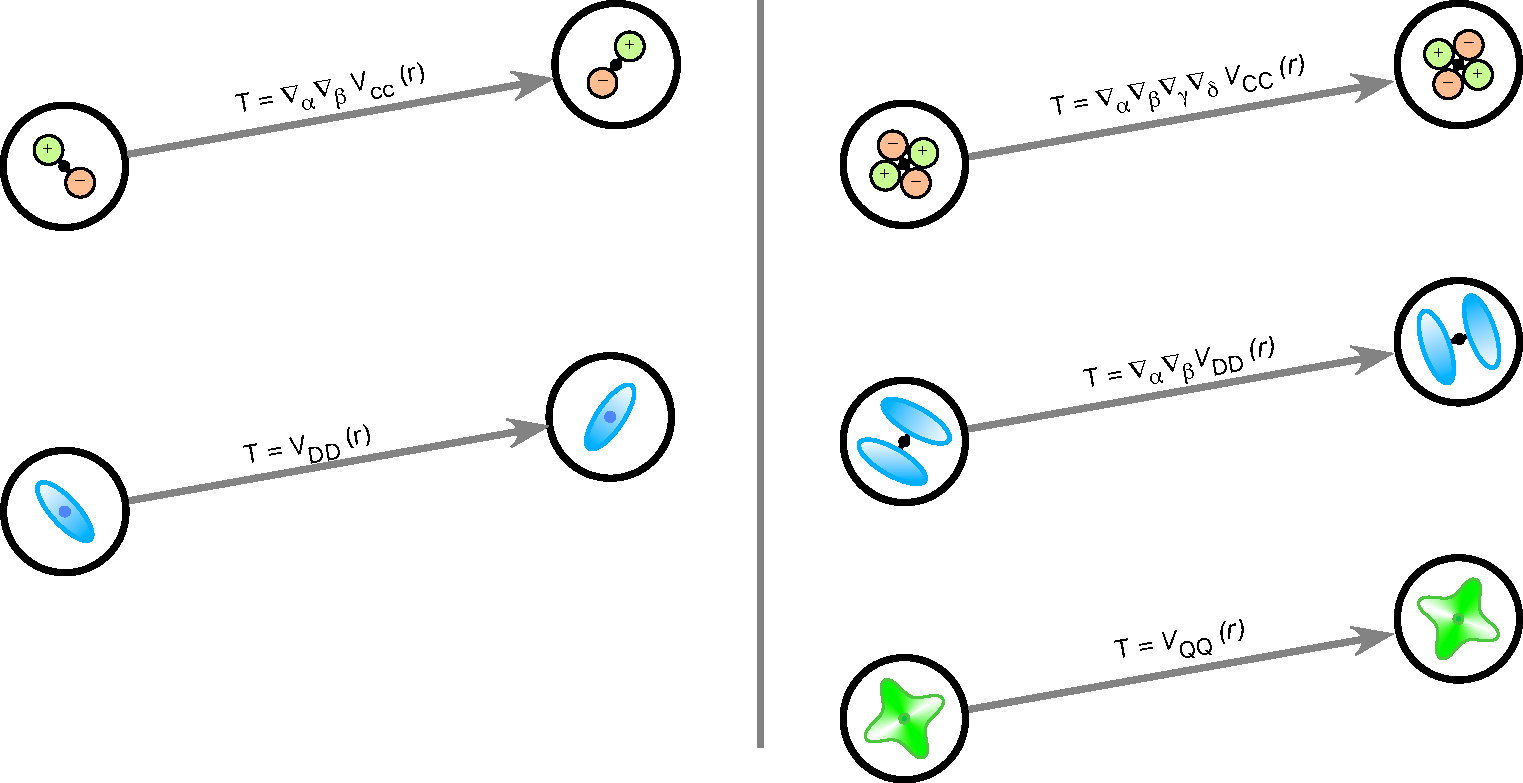
\includegraphics[width=\linewidth]{Tensors}
\caption{In the real-space electrostatic methods, the molecular dipole
  tensor, $\mathbf{T}_{\alpha\beta}(r)$, is not the same for
  charge-charge interactions as for point dipoles (left panel). The
  same holds true for the molecular quadrupole tensor (right panel),
  $\mathbf{T}_{\alpha\beta\gamma\delta}(r)$, which can have distinct
  forms if the molecule is represented by charges, dipoles, or point
  quadrupoles.}
\label{fig:tensor}
\end{figure}
In the case where point charges are interacting via an electrostatic
kernel, $v(r)$, the effective {\it molecular} dipole tensor,
$\mathbf{T}$ is obtained from two successive applications of the
gradient operator to the electrostatic kernel,
\begin{eqnarray}
\mathbf{T}_{\alpha \beta}(r) &=&  \nabla_\alpha \nabla_\beta
                               \left(v(r)\right)  \\
  &=& \delta_{\alpha \beta}
\left(\frac{1}{r} v^\prime(r) \right) + \frac{r_{\alpha}
  r_{\beta}}{r^2} \left( v^{\prime \prime}(r) - \frac{1}{r}
  v^{\prime}(r) \right)
\label{dipole-chargeTensor}
\end{eqnarray}
where $v(r)$ may be either the bare kernel ($1/r$) or one of the
modified (Wolf or DSF) kernels.  This tensor describes the effective
interaction between molecular dipoles ($\mathbf{D}$) in Gaussian units
as $-\mathbf{D} \cdot \mathbf{T} \cdot \mathbf{D}$.

When utilizing any of the three new real-space methods for point
\textit{dipoles}, the tensor is explicitly constructed,
\begin{equation}
\mathbf{T}_{\alpha \beta}(r)  =  \delta_{\alpha \beta} v_{21}(r) +
\frac{r_{\alpha} r_{\beta}}{r^2} v_{22}(r) 
\label{dipole-diopleTensor}
\end{equation}
where the functions $v_{21}(r)$ and $v_{22}(r)$ depend on the level of
the approximation.\cite{PaperI,PaperII} Although the Taylor-shifted
(TSF) and gradient-shifted (GSF) models produce to the same $v(r)$
function for point charges, they have distinct forms for the
dipole-dipole interaction.
 
Using a constitutive relation, the polarization density
$\mathbf{P}(\mathbf{r})$ is given by,
\begin{equation}
\mathbf{P}(\mathbf{r}) = \epsilon_o \chi_D
\left(\mathbf{E}^\circ(\mathbf{r}) + \frac{1}{4\pi\epsilon_o} \int
  d\mathbf{r}^\prime \mathbf{T}(\mathbf{r}-\mathbf{r}^\prime ) \cdot \mathbf{P}(\mathbf{r}^\prime)\right).
\label{constDipole}
\end{equation}
Note that $\chi_D$ explicitly depends on the details of the dipole
interaction tensor.  Neumann \textit{et al.}
\cite{NeumannI83,NeumannII83,Neumann84,Neumann85} derived an elegant
way to modify the fluctuation formula to correct for approximate
interaction tensors. This correction was derived using a Fourier
representation of the interaction tensor,
$\tilde{\mathbf{T}}(\mathbf{k})$, and involves the quantity,
\begin{equation}
 A = \frac{3}{4\pi}\tilde{\mathbf{T}}(0) = \frac{3}{4\pi} \int_V
 d\mathbf{r} \mathbf{T}(\mathbf{r})
 \label{dipCorrFactor}
\end{equation}
which is the $k \rightarrow 0$ limit of $\tilde{\mathbf{T}}$.  Using
this quantity (originally called $Q$ in
Refs.~\cite{NeumannI83,NeumannII83,Neumann84,Neumann85}), the
dielectric constant can be computed
\begin{equation}
\epsilon = \frac{3+(A + 2)(\epsilon_{CB}-1)}{3 + (A -1)(\epsilon_{CB}-1)}
\label{correctionFormula}
\end{equation}
where $\epsilon_{CB}$ is the widely-used conducting boundary
expression for the dielectric constant,
\begin{equation}
\epsilon_{CB} = 1 + \frac{\braket{\bf{M}^2}-{\braket{\bf{M}}}^2}{3
  \epsilon_o V k_B T} = 1 + \alpha_{D}
\label{conductingBoundary}
\end{equation}
Eqs.~(\ref{correctionFormula}) and (\ref{conductingBoundary}) allows
estimation of the static dielectric constant from fluctuations easily
computed directly from simulations.

We have utilized the Neumann \textit{et al.} approach for the three
new real-space methods, and obtain method-dependent correction
factors.  The expression for the correction factor also depends on
whether the simulation involves point charges or point dipoles to
represent the molecular dipoles.  These corrections factors are 
listed in Table~\ref{tab:A}. We note that the GSF correction factor for
point dipoles has been independently derived by Stenqvist \textit{et
  al.}\cite{Stenqvist:2015ph}

\begin{sidewaystable}[tpb]
	\begin{center}
  	\caption{Expressions for the dipolar correction factor ($A$) for the
    real-space electrostatic methods in terms of the damping parameter 
    ($\alpha$) and the cutoff radius ($r_c$).  The Ewald-Kornfeld result 
    derived in Refs.\cite{Adams80,Adams81,NeumannI83} is shown
    for comparison using the Ewald convergence parameter ($\kappa$)
    and the real-space cutoff value ($r_c$). } 
		\label{tab:A}
	\begin{tabular}{l|c|c}
	%\toprule
	\hline       
	& \multicolumn{2}{c}{Molecular Representation} \\ 
	Method & point charges & point dipoles  \\ \hline
	\colrule
 		Shifted Potental (SP) & $ \mathrm{erf}(r_c \alpha) - \frac{2
                               \alpha r_c}{\sqrt{\pi}} e^{-\alpha^2
                               r_c^2}$ & $\mathrm{erf}(r_c \alpha)
                                         -\frac{2 \alpha
                                         r_c}{\sqrt{\pi}}\left(1+\frac{2\alpha^2
                                         {r_c}^2}{3}
                                         \right)e^{-\alpha^2{r_c}^2}
                                         $\\ \colrule
	Gradient-shifted  (GSF) & 1 & $\mathrm{erf}(\alpha  r_c)-\frac{2
                              \alpha  r_c}{\sqrt{\pi}}  \left(1 +
                              \frac{2 \alpha^2 r_c^2}{3} +
                              \frac{\alpha^4
                              r_c^4}{3}\right)e^{-\alpha^2 r_c^2} $ \\ \colrule
	Taylor-shifted  (TSF) & 1 & 1  \\ \colrule
	Spherical Cutoff (SC)& $\mathrm{erf}(r_c \alpha) -
                        \frac{2 \alpha r_c}{\sqrt{\pi}} e^{-\alpha^2
                        r_c^2}$ & $\mathrm{erf}(r_c \alpha) -
                        \frac{2 \alpha r_c}{\sqrt{\pi}} e^{-\alpha^2
                        r_c^2}$ \\ 
	Ewald-Kornfeld (EK) & $\mathrm{erf}(r_c \kappa) -
                      \frac{2 \kappa r_c}{\sqrt{\pi}} e^{-\kappa^2
                      r_c^2}$ & $\mathrm{erf}(r_c \kappa) -
                      \frac{2 \kappa r_c}{\sqrt{\pi}} e^{-\kappa^2
                      r_c^2}$  \\ \hline
%\botrule
	\end{tabular}
	\end{center}
\end{sidewaystable}
Note that for point charges, the GSF and TSF methods produce estimates
of the dielectric that need no correction, and the TSF method likewise
needs no correction for point dipoles. 

\section{Quadrupolar Fluids and the Quadrupolar Susceptibility}
\subsection{Response to External Perturbations}

A molecule with a permanent quadrupole, $\mathsf{q}$, will align in
the presence of an electric field gradient $\nabla\mathbf{E}$.  The
anisotropic polarization of the quadrupole is given
by,\cite{AduGyamfi78,AduGyamfi81}
\begin{equation}
\braket{\mathsf{q}} - \frac{\mathbf{I}}{3}
\mathrm{Tr}(\mathsf{q}) = \epsilon_o \alpha_q \nabla\mathbf{E},
\end{equation}
where $\alpha_q = q_o^2 / 15 \epsilon_o k_B T $ is a molecular quadrupole
polarizablity and $q_o$ is an effective quadrupole moment for the molecule,
\begin{equation}
 q_o^2 = 3 \mathsf{q}:\mathsf{q} - \mathrm{Tr}(\mathsf{q})^2.
\end{equation}

In the presence of an external field gradient, a system of quadrupolar
molecules also organizes with an anisotropic polarization,
\begin{equation}
\mathsf{Q} - \frac{\mathbf{I}}{3} \mathrm{Tr}(\mathsf{Q}) =  \epsilon_o
\alpha_Q  \nabla\mathbf{E}
\end{equation}
where $\mathsf{Q}$ is the traced quadrupole density of the system and
$\alpha_Q$ is a macroscopic quadrupole polarizability which has
dimensions of $\mathrm{length}^{-2}$. Equivalently, the traceless form
may be used,
\begin{equation}
\mathsf{\Theta} = 3 \epsilon_o  \alpha_Q \nabla\mathbf{E},
\label{pertQuad}
\end{equation} 
where
$\mathsf{\Theta} = 3\mathsf{Q} - \mathbf{I} \mathrm{Tr}(\mathsf{Q})$
is the traceless tensor that also describes the system quadrupole
density.  It is this tensor that will be utilized to derive correction
factors below.

\subsection{Fluctuation Formula}
As in the dipolar case, we may define a system quadrupole moment,
$\mathsf{M}_Q = \sum_i \mathsf{q}_i$ and the traced quadrupolar
density, $\mathsf{Q} = \mathsf{M}_Q / V$.  A fluctuation formula can
be written for a system comprising quadrupolar
molecules,\cite{LoganI81,LoganII82,LoganIII82}
\begin{equation}
\mathsf{Q} - \frac{\mathbf{I}}{3} \mathrm{Tr}(\mathsf{Q}) = \epsilon_o
\frac{\braket{\mathsf{M}_Q^2}-{\braket{\mathsf{M}_Q}}^2}{15 \epsilon_o
  V k_B T} \nabla\mathbf{E}.
\label{flucQuad}
\end{equation}
Some care is needed in the definitions of the averaged quantities.  These
refer to the effective quadrupole moment of the system, and they are
computed as follows,
\begin{align}
\braket{\mathsf{M}_Q^2} &= \braket{3 \mathsf{M}_Q:\mathsf{M}_Q -
  \mathrm{Tr}(\mathsf{M}_Q)^2 }\\
\braket{\mathsf{M}_Q}^2 &= 3 \braket{\mathsf{M}_Q}:\braket{\mathsf{M}_Q} -
\mathrm{Tr}(\braket{\mathsf{M}_Q})^2
\label{eq:flucQuad}
\end{align}
The macroscopic quadrupolarizability is given by,
\begin{equation}
  \alpha_Q = \frac{\braket{\mathsf{M}_Q^2}-{\braket{\mathsf{M}_Q}}^2}{15 \epsilon_o V k_B T}
\label{propConstQuad}
\end{equation}
This relationship between a macroscopic property of a quadrupolar
fluid and microscopic fluctuations should be true even when the
applied field gradient $\nabla \mathbf{E} \rightarrow 0$.

\subsection{Correction Factors}
In this section we generalize the treatment of Neumann \textit{et al.}
for quadrupolar fluids. Interactions involving multiple quadrupoles
are rank 4 tensors, and we therefore describe quantities in this
section using Einstein notation.

In the presence of a uniform external field gradient,
$\partial_\alpha {E}^\circ_\beta $, the total field gradient at
$\mathbf{r}$ depends on the quadrupole polarization density at all
other points in the system,
\begin{equation}
\partial_\alpha E_\beta(\mathbf{r}) = \partial_\alpha
{E}^\circ_\beta(\mathbf{r}) + \frac{1}{8\pi \epsilon_o}\int
T_{\alpha\beta\gamma\delta}({\mathbf{r}-\mathbf{r}^\prime})
Q_{\gamma\delta}(\mathbf{r}^\prime) d\mathbf{r}^\prime 
\label{gradMaxwell}
\end{equation}
where and $T_{\alpha\beta\gamma\delta}$ is the quadrupole interaction
tensor connecting quadrupoles at $\mathbf{r}^\prime$ with the point of
interest ($\mathbf{r}$).

In simulations of quadrupolar fluids, the molecular quadrupoles may be
represented by closely-spaced point charges, by multiple point
dipoles, or by a single point quadrupole (see
Fig. \ref{fig:tensor}).  In the case where point charges are
interacting via an electrostatic kernel, $v(r)$, the effective
molecular quadrupole tensor can obtained from four successive
applications of the gradient operator to the electrostatic kernel,
\begin{eqnarray}
T_{\alpha\beta\gamma\delta}(\mathbf{r}) &=& \nabla_\alpha \nabla_\beta
                                   \nabla_\gamma \nabla_\delta v(r) \\
 &=& \left(\delta_{\alpha\beta}\delta_{\gamma\delta} +
     \delta_{\alpha\gamma}\delta_{\beta\delta}+
     \delta_{\alpha\delta}\delta_{\beta\gamma}\right)\left(-\frac{v^\prime(r)}{r^3}
     + \frac{v^{\prime \prime}(r)}{r^2}\right) \nonumber \\
 & &+ \left(\delta_{\alpha\beta} r_\gamma r_\delta + 5  \mathrm{~permutations}
     \right) \left(\frac{3v^\prime(r)}{r^5}-\frac{3v^{\prime \prime}(r)}{r^4} +
     \frac{v^{\prime \prime \prime}(r)}{r^3}\right) \nonumber \\
 & &+ r_\alpha r_\beta r_\gamma r_\delta
     \left(-\frac{15v^\prime(r)}{r^7}+\frac{15v^{\prime \prime}(r)}{r^6}-\frac{6v^{\prime
     \prime \prime}(r)}{r^5} + \frac{v^{\prime \prime \prime \prime}(r)}{r^4}\right),
\label{quadCharge}
\end{eqnarray}
where $v(r)$ can either be the electrostatic kernel ($1/r$) or one of
the modified (Wolf or DSF) kernels.  

Similarly, when representing quadrupolar molecules with multiple point
\textit{dipoles}, the molecular quadrupole interaction tensor can be
obtained using two successive applications of the gradient operator to
the dipole interaction tensor,
\begin{eqnarray}
T_{\alpha\beta\gamma\delta}(\mathbf{r}) &=& \nabla_\alpha \nabla_\beta
                                            T_{\gamma\delta}(\mathbf{r}) \\ 
& = & \delta_{\alpha\beta}\delta_{\gamma\delta} \frac{v^\prime_{21}(r)}{r} +
      \left(\delta_{\alpha\gamma}\delta_{\beta\delta}+
      \delta_{\alpha\delta}\delta_{\beta\gamma}\right)\frac{v_{22}(r)}{r^2}
      \nonumber\\ 
 & &+ \delta_{\gamma\delta} r_\alpha r_\beta
     \left(\frac{v^{\prime \prime}_{21}(r)}{r^2}-\frac{v^\prime_{21}(r)}{r^3} \right)\nonumber \\
 & &+\left(\delta_{\alpha\beta} r_\gamma r_\delta +
     \delta_{\alpha\gamma} r_\beta r_\delta  +\delta_{\alpha\delta}
     r_\gamma r_\beta + \delta_{\beta\gamma} r_\alpha r_\delta
     +\delta_{\beta\delta} r_\alpha r_\gamma  \right)
     \left(\frac{v^\prime_{22}(r)}{r^3}-\frac{2v_{22}(r)}{r^4}\right)
     \nonumber \\
 & &+ r_\alpha r_\beta r_\gamma r_\delta
     \left(\frac{v^{\prime
     \prime}_{22}(r)}{r^4}-\frac{5v^\prime_{22}(r)}{r^5}+\frac{8v_{22}(r)}{r^6}\right),
\label{quadDip}
\end{eqnarray}
where $T_{\gamma\delta}(\mathbf{r})$ is a dipole-dipole interaction
tensor that depends on the level of the
approximation.\cite{PaperI,PaperII} Similarly $v_{21}(r)$ and
$v_{22}(r)$ are the radial function for different real space cutoff
methods defined in the Chapter 2.\cite{PaperI}

For quadrupolar liquids modeled using point quadrupoles, the
interaction tensor can be constructed as,
\begin{eqnarray}
T_{\alpha\beta\gamma\delta}(\mathbf{r}) &=&
                                              \left(\delta_{\alpha\beta}\delta_{\gamma\delta}
                                              +
                                              \delta_{\alpha\gamma}\delta_{\beta\delta}+
                                              \delta_{\alpha\delta}\delta_{\beta\gamma}\right)v_{41}(r)
                                              + (\delta_{\gamma\delta} r_\alpha r_\beta +  \mathrm{ 5\; permutations}) \frac{v_{42}(r)}{r^2} \nonumber \\  
& & + r_\alpha r_\beta r_\gamma r_\delta  \left(\frac{v_{43}(r)}{r^4}\right), 
\label{quadRadial}
\end{eqnarray}
where again $v_{41}(r)$, $v_{42}(r)$, and $v_{43}(r)$ are radial
functions defined in Chapter 2. \cite{PaperI} Note that
these radial functions have different functional forms depending on
the level of approximation being employed.

The integral in Eq.~(\ref{gradMaxwell}) can be divided into two
parts, $|\mathbf{r}-\mathbf{r}^\prime|\rightarrow 0 $ and
$|\mathbf{r}-\mathbf{r}^\prime|> 0$. Since the self-contribution to
the field gradient vanishes at the singularity (see the supporting
information), Eq.~(\ref{gradMaxwell}) can be written as,
\begin{equation}
\partial_\alpha E_\beta(\mathbf{r}) = \partial_\alpha {E}^\circ_\beta(\mathbf{r}) +
  \frac{1}{8\pi \epsilon_o}\int\limits_{|\mathbf{r}-\mathbf{r}^\prime|> 0 }
  T_{\alpha\beta\gamma\delta}(\mathbf{r}-\mathbf{r}^\prime)
  {Q}_{\gamma\delta}(\mathbf{r}^\prime) d\mathbf{r}^\prime.
\end{equation}
If $\mathbf{r} = \mathbf{r}^\prime$ is excluded from the integration,
the total gradient can be most easily expressed in terms of
traceless quadrupole density as below,\cite{LoganI81}
\begin{equation}
\partial_\alpha E_\beta(\mathbf{r}) = \partial_\alpha
{E}^\circ_\beta(\mathbf{r}) + \frac{1}{24\pi
  \epsilon_o}\int\limits_{|\mathbf{r}-\mathbf{r}^\prime|> 0 }
T_{\alpha\beta\gamma\delta}(\mathbf{r}-\mathbf{r}^\prime) \Theta_{\gamma\delta}(\mathbf{r}') d\mathbf{r}^\prime,
\end{equation}
where
$\Theta_{\alpha\beta} = 3Q_{\alpha\beta} - \delta_{\alpha\beta}Tr(Q)$
is the traceless quadrupole density. In analogy to
Eq.~(\ref{pertQuad}) above, the quadrupole polarization density may
now be related to the quadrupolar susceptibility, $\chi_Q$,
\begin{equation}
\frac{1}{3}{\Theta}_{\alpha\beta}(\mathbf{r}) = \epsilon_o {\chi}_Q
\left[\partial_\alpha {E}^\circ_\beta(\mathbf{r}) + \frac{1}{24\pi
    \epsilon_o}\int\limits_{|\mathbf{r}-\mathbf{r}^\prime|> 0 }
  T_{\alpha\beta\gamma\delta}(\mathbf{r}-\mathbf{r}^\prime)
  \Theta_{\gamma\delta}(\mathbf{r}^\prime) d\mathbf{r}^\prime \right].
\end{equation}
For periodic boundaries and with a uniform imposed
$\partial_\alpha E^\circ_\beta$, the quadrupole density
${\Theta}_{\alpha\beta}$ will be uniform over the entire space. After
performing a Fourier transform (see the Appendix in
Ref.\cite{NeumannI83}) we obtain,
\begin{equation}
\frac{1}{3}\tilde{\Theta}_{\alpha\beta}(\mathbf{k})=
\epsilon_o {\chi}_Q \left[{\partial_\alpha
    \tilde{E}^\circ_\beta}(\mathbf{k})+ \frac{1}{24\pi
    \epsilon_o} \tilde{T}_{\alpha\beta\gamma\delta}(\mathbf{k})
 \tilde{\Theta}_{\gamma\delta}(\mathbf{k})\right].
\label{fourierQuad}
\end{equation} 
If the applied field gradient is homogeneous over the entire volume,
${\partial_ \alpha \tilde{E}^\circ_\beta}(\mathbf{k}) = 0 $ except at
$ \mathbf{k} = 0$. Similarly, the quadrupolar polarization density can
also considered uniform over entire space. As in the dipolar case,
\cite{NeumannI83} the only relevant contribution from the interaction
tensor will also be when $\mathbf{k} = 0$. Therefore Eq.~(\ref{fourierQuad}) can be written as,
\begin{equation}
\frac{1}{3}\tilde{\Theta}_{\alpha\beta}(\mathrm{0})=
\epsilon_o {\chi}_Q \left[{\partial_\alpha
    \tilde{E}^\circ_\beta}(\mathrm{0})+ \frac{1}{24\pi
    \epsilon_o} \tilde{T}_{\alpha\beta\gamma\delta}(\mathrm{0})
 \tilde{\Theta}_{\gamma\delta}(\mathrm{0})\right].
\label{fourierQuadZeroK}
\end{equation} 
The quadrupolar tensor
$\tilde{T}_{\alpha\beta\gamma\delta}(\mathrm{0})$ is a rank 4 tensor
with 81 elements. The only non-zero elements, however, are those with
two doubly-repeated indices, \textit{i.e.}
$\tilde{T}_{aabb}(\mathrm{0})$ and all permutations of these indices.
The special case of quadruply-repeated indices,
$\tilde{T}_{aaaa}(\mathrm{0})$ also survives (see appendix
\ref{ap:quadContraction}). Furthermore, for the both diagonal and
non-diagonal components of the quadrupolar polarization
$\tilde{\Theta}_{\alpha\beta}$, we can contract the second term in
Eq.~\ref{fourierQuadZeroK} (see appendix
\ref{ap:quadContraction}):
\begin{equation}
\tilde{T}_{\alpha\beta\gamma\delta}(\mathrm{0})\tilde{\Theta}_{\gamma\delta}(\mathrm{0})=
8 \pi \mathrm{B} \tilde{\Theta}_{\alpha\beta}(\mathrm{0}).
\label{quadContraction}
\end{equation}
Here $\mathrm{B} = \tilde{T}_{abab}(\mathrm{0}) / 4 \pi$ for
$a \neq b$.  Using this quadrupolar contraction we can solve Eq.~(\ref{fourierQuadZeroK}) as follows
\begin{eqnarray}
\frac{1}{3}\tilde{\Theta}_{\alpha\beta}(\mathrm{0}) &=& \epsilon_o
                                                      {\chi}_Q
                                                      \left[{\partial_\alpha
                                                      \tilde{E}^\circ_\beta}(\mathrm{0})+
                                                      \frac{\mathrm{B}}{3
                                                      \epsilon_o} 
                                                      {\tilde{\Theta}}_{\alpha\beta}(\mathrm{0})\right]
                                                      \nonumber \\                                                    
&=& \left[\frac{\epsilon_o {\chi}_Q} {1-{\chi}_Q \mathrm{B}}\right]
{\partial_\alpha \tilde{E}^\circ_\beta}(\mathrm{0}).
\label{fourierQuad2}
\end{eqnarray}
In real space, the correction factor is found to be,
\begin{equation}
\mathrm{B} = \frac{1}{4 \pi} \tilde{T}_{abab}(0) = \frac{1}{4 \pi} \int_V {T}_{abab}(\mathbf{r}) d\mathbf{r},
\end{equation}

which has been integrated over the interaction volume $V$ and has
units of $\mathrm{length}^{-2}$.

In terms of the traced quadrupole moment, Eq.~(\ref{fourierQuad2})
can be written,
\begin{equation}
\mathsf{Q} - \frac{\mathbf{I}}{3} \mathrm{Tr}(\mathsf{Q})
= \frac{\epsilon_o {\chi}_Q}{1-  {\chi}_Q \mathrm{B}} \nabla \mathbf{E}^\circ
\label{tracedConstQuad}
\end{equation}
Comparing (\ref{tracedConstQuad}) and (\ref{flucQuad}) we obtain,
\begin{equation}
\frac{\braket{\mathsf{M}_Q^2}-{\braket{\mathsf{M}_Q}}^2}{15 \epsilon_o
  V k_B T} = \frac{\chi_Q} {1 - \chi_Q \mathrm{B}},
\end{equation}
or equivalently,
\begin{equation}
\chi_Q = \frac{\braket{\mathsf{M}_Q^2}-{\braket{\mathsf{M}_Q}}^2}{15 \epsilon_o
  V k_B T} \left(1 + \mathrm{B} \frac{\braket{\mathsf{M}_Q^2}-{\braket{\mathsf{M}_Q}}^2}{15 \epsilon_o
  V k_B T} \right)^{-1}
\label{eq:finalForm}
\end{equation}
Eq.~(\ref{eq:finalForm}) now expresses a bulk property (the
quadrupolar susceptibility, $\chi_Q$) in terms of a fluctuation in the
system quadrupole moment and a quadrupolar correction factor
($\mathrm{B}$).  The correction factors depend on the cutoff method
being employed in the simulation, and these are listed in Table~\ref{tab:B}.

In terms of the macroscopic quadrupole polarizability, $\alpha_Q$,
which may be thought of as the ``conducting boundary'' version of the
susceptibility,
\begin{equation}
\chi_Q = \frac{\alpha_Q}{1 + \mathrm{B} \alpha_Q}.
\label{eq:quadrupolarSusceptiblity}
\end{equation}
If an electrostatic method produces $\mathrm{B} \rightarrow 0$, the computed
quadrupole polarizability and quadrupole susceptibility converge to
the same value.

\begin{sidewaystable}[tpb]
\begin{center}
  \caption{Expressions for the quadrupolar correction factor
    ($\mathrm{B}$) for the real-space electrostatic methods in terms
    of the damping parameter ($\alpha$) and the cutoff radius
    ($r_c$). The units of the correction factor are
    $ \mathrm{length}^{-2}$ for quadrupolar fluids.}
\label{tab:B}
\begin{tabular}{l|c|c|c} \hline %\toprule
\multirow{2}{*}{Method} &  \multicolumn{3}{c}{Molecular Representation} \\ 
 & charges & dipoles & quadrupoles \\ \hline \colrule
Shifted Potental (SP) & $ -\frac{8 \alpha^5 {r_c}^3e^{-\alpha^2 r_c^2}}{15\sqrt{\pi}} $ &  $-  \frac{3 \mathrm{erfc(r_c\alpha)}}{5{r_c}^2}- \frac{2 \alpha e^{-\alpha^2 r_c^2}(9+6\alpha^2 r_c^2+4\alpha^4 r_c^4)}{15{\sqrt{\pi}r_c}}$& $ -\frac{16 \alpha^7 {r_c}^5 e^{-\alpha^2 r_c^2                                 }}{45\sqrt{\pi}}$  \\
Gradient-shifted  (GSF) & $- \frac{8 \alpha^5 {r_c}^3e^{-\alpha^2 r_c^2}}{15\sqrt{\pi}} $ & 0 &  $-\frac{4{\alpha}^7{r_c}^5 e^{-\alpha^2 r_c^2}(-1+2\alpha ^2 r_c^2)}{45\sqrt{\pi}}$\\
Taylor-shifted  (TSF) &  $ -\frac{8 \alpha^5 {r_c}^3e^{-\alpha^2 r_c^2}}{15\sqrt{\pi}} $ & $\frac{4\;\mathrm{erfc(\alpha r_c)}}{{5r_c}^2} + \frac{8\alpha e^{-\alpha^2{r_c}^2}\left(3+ 2\alpha^2 {r_c}^2 +\alpha^4{r_c}^4 \right)}{15\sqrt{\pi}r_c}$ & $\frac{2\;\mathrm{erfc}(\alpha r_c )}{{r_c}^2} + \frac{4{\alpha}e^{-\alpha^2 r_c^2}\left(45 + 30\alpha ^2 {r_c}^2 + 12\alpha^4 {r_c}^4 + 3\alpha^6 {r_c}^6 + 2 \alpha^8 {r_c}^8\right)}{45\sqrt{\pi}{r_c}}$ \\
\colrule
Spherical Cutoff (SC) &$ -\frac{8 \alpha^5
                        {r_c}^3e^{-\alpha^2 r_c^2}}{15\sqrt{\pi}} $ &$ -\frac{8 \alpha^5
                        {r_c}^3e^{-\alpha^2 r_c^2}}{15\sqrt{\pi}} $ & $ -\frac{8 \alpha^5
                        {r_c}^3e^{-\alpha^2 r_c^2}}{15\sqrt{\pi}} $\\ 
Ewald-Kornfeld (EK) & $ -\frac{8 \kappa^5 {r_c}^3e^{-\kappa^2 r_c^2}}{15\sqrt{\pi}}$& $ -\frac{8 \kappa^5 {r_c}^3e^{-\kappa^2 r_c^2}}{15\sqrt{\pi}}$ & $ -\frac{8 \kappa^5 {r_c}^3e^{-\kappa^2 r_c^2}}{15\sqrt{\pi}}$ \\
\hline
%\botrule
\end{tabular}
\end{center}
\end{sidewaystable}

\section{Screening of Charges by Multipolar Fluids}
\label{sec:PMF}
In a dipolar fluid, the static dielectric constant is also a measure
of the ability of the fluid to screen charges from one another.  A set
of point charges creates an inhomogeneous field in the fluid, and the
fluid responds to this field as if it was created externally or via
local polarization fluctuations. For this reason, the dielectric
constant can be used to estimate an effective potential between two
point charges ($C_i$ and $C_j$) embedded in the fluid,
\begin{equation}
U_\mathrm{effective} = \frac{C_i C_j}{4 \pi \epsilon_0 \epsilon
  r_{ij}}.
\label{eq:effectivePot}
\end{equation}

The same set of point charges can also create an inhomogeneous field
\textit{gradient}, and this will cause a response in a quadrupolar
fluid that will also cause an effective screening. As discussed above,
however, the relevant phyiscal property in quadrupolar fluids is the
susceptibility, $\chi_Q$.  The screening dielectric associated with
the quadrupolar susceptibility is defined as,\cite{Ernst92}
\begin{equation}
\epsilon = 1 + \chi_Q G = 1 + G \frac{\alpha_Q}{1 + \alpha_Q  B}
\label{eq:dielectricFromQuadrupoles}
\end{equation}
where $G$ is a geometrical factor that depends on the geometry of the
field perturbation,
\begin{equation}
G = \frac{\int_V \left| \nabla \mathbf{E}^\circ \right|^2 d\mathbf{r}}
{\int_V \left|\mathbf{E}^\circ\right|^2 d\mathbf{r}}
\end{equation}
integrated over the interaction volume. Note that this geometrical
factor is also required to compute effective dielectric constants even
when the field gradient is homogeneous over the entire sample.

To measure effective screening in a multipolar fluid, we compute an
effective interaction potential, the potential of mean force (PMF),
between positively and negatively charged ions when they screened by
the intervening fluid.  The PMF is obtained from a sequence of
simulations in which two ions are constrained to a fixed distance, and
the average constraint force to hold them at a fixed distance $r$ is
collected during a long simulation,\cite{Wilfred07}
\begin{equation}
w(r) = \int_{r_o}^{r}\left\langle \frac{\partial f}{\partial r^\prime}
\right\rangle_{r^\prime} dr^\prime + 2k_BT \ln\left(\frac{r}{r_o}\right) + w(r_o),
\label{eq:pmf}
\end{equation}
where $\braket{\partial f/\partial r^\prime}_{r^\prime}$ is the mean
constraint force required to hold the ions at distance $r^\prime$,
$2k_BT \log(r/r_o)$ is the Fixman factor,\cite{Fixman:1974fk} and
$r_o$ is a reference position (usually taken as a large separation
between the ions). If the dielectric constant is a good measure of the
screening at all inter-ion separations, we would expect $w(r)$ to have
the form in Eq.~(\ref{eq:effectivePot}).  Because real fluids are not
continuum dielectrics, the effective dielectric constant is a function
of the inter-ionic separation,
\begin{equation}
\epsilon(r) = \frac{u_\mathrm{raw}(r) - u_\mathrm{raw}(r_o) }{w(r) - w(r_o)} 
\end{equation}
where $u_\mathrm{raw}(r)$ is the direct charge-charge interaction
potential that is in use during the simulation.  $\epsilon(r)$ may
vary considerably from the bulk estimates at short distances, although
it should converge to the bulk value as the separation between the
ions increases.

\section{Simulation Methodology}

To test the formalism developed in the preceding sections, we have
carried out computer simulations using three different techniques: i)
simulations in the presence of external fields, ii) equilibrium
calculations of box moment fluctuations, and iii) potentials of mean
force (PMF) between embedded ions. In all cases, the fluids were
composed of point multipoles protected by a Lennard-Jones potential.
The parameters used in the test systems are given in Table~\ref{Tab:C}.

\begin{sidewaystable}
  \caption{\label{Tab:C}The parameters used in simulations to evaluate
    the dielectric response of the new real-space methods.} 
\begin{tabularx}{\textwidth}{r|cc|YYccc|Yccc} \hline
             & \multicolumn{2}{c|}{LJ parameters} &
             \multicolumn{5}{c|}{Electrostatic moments} & & & & \\
 Test system & $\sigma$& $\epsilon$ & $C$ & $D$  &
 $Q_{xx}$ & $Q_{yy}$ & $Q_{zz}$ & mass  & $I_{xx}$ & $I_{yy}$ &
 $I_{zz}$ \\ \cline{6-8}\cline{10-12}
 & (\AA) & (kcal/mol) & (e) & (debye) & \multicolumn{3}{c|}{(debye \AA)} & (amu) & \multicolumn{3}{c}{(amu
 \AA\textsuperscript{2})} \\ \hline
    Dipolar fluid & 3.41 & 0.2381 & - & 1.4026 &-&-&-& 39.948 & 11.613 & 11.613 & 0.0 \\
Quadrupolar fluid & 2.985 & 0.265 & - & - & 0.0 & 0.0 &-2.139 & 18.0153 & 43.0565 & 43.0565 & 0.0  \\
              \ce{q+} & 1.0 & 0.1 & +1 & - & - & - & - & 22.98 & - & - & - \\
              \ce{q-} & 1.0 & 0.1 & -1 & - & - & - & - & 22.98 & - & - & - \\ \hline
\end{tabularx}
\end{sidewaystable}

The first of the test systems consists entirely of fluids of point
dipolar or quadrupolar molecules in the presence of constant field or
field gradients.  Since there are no isolated charges within the
system, the divergence of the field will be zero, \textit{i.e.}
$\vec{\nabla} \cdot \mathbf{E} = 0$. This condition can be satisfied
by using the relatively simple applied potential as described in the
supporting information.

When a constant electric field or field gradient is applied to the
system, the molecules align along the direction of the applied field,
and polarize to a degree determined both by the strength of the field
and the fluid's polarizibility.  We have calculated ensemble averages
of the box dipole and quadrupole moments as a function of the strength
of the applied fields.  If the fields are sufficiently weak, the
response is linear in the field strength, and one can easily compute
the polarizability directly from the simulations.

The second set of test systems consists of equilibrium simulations of
fluids of point dipolar or quadrupolar molecules simulated in the
absence of any external perturbation. The fluctuation of the ensemble
averages of the box multipolar moment was calculated for each of the
multipolar fluids. The box multipolar moments were computed as simple
sums over the instantaneous molecular moments, and fluctuations in
these quantities were obtained from Eqs.~(\ref{eq:flucDip}) and
(\ref{eq:flucQuad}). The macroscopic polarizabilities of the system at
a were derived using Eqs.(\ref{flucDipole}) and (\ref{flucQuad}).

The final system consists of dipolar or quadrupolar fluids with two
oppositely charged ions embedded within the fluid. These ions are
constrained to be at fixed distance throughout a simulation, although
they are allowed to move freely throughout the fluid while satisfying
that constraint. Separate simulations were run at a range of
constraint distances. A dielectric screening factor was computed using
the ratio between the potential between the two ions in the absence of
the fluid medium and the PMF obtained from the simulations.

We carried out these simulations for all three of the new real-space
electrostatic methods (SP, GSF, and TSF) that were developed in the
Chapter 2 (Ref. cite{PaperI}) in the series. The radius of
the cutoff sphere was taken to be 12~\AA. Each of the real space
methods also depends on an adjustable damping parameter $\alpha$ (in
units of $\mathrm{length}^{-1}$).  We have selected ten different
values of damping parameter: 0.0, 0.05, 0.1, 0.15, 0.175, 0.2, 0.225,
0.25, 0.3, and 0.35~\AA$^{-1}$ in our simulations of the dipolar
liquids, while four values were chosen for the quadrupolar fluids:
0.0, 0.1, 0.2, and 0.3~\AA$^{-1}$.

For each of the methods and systems listed above, a reference
simulation was carried out using a multipolar implementation of the
Ewald sum.\cite{Smith82,Smith98} A default tolerance of
$1 \times 10^{-8}$~kcal/mol was used in all Ewald calculations,
resulting in Ewald coefficient 0.3119~\AA$^{-1}$ for a cutoff radius
of 12~\AA.  All of the electrostatics and constraint methods were
implemented in our group's open source molecular simulation program,
OpenMD,\cite{Meineke05, openmd} which was used for all calculations in
this work.

Dipolar systems contained 2048 Lennard-Jones-protected point dipolar
(Stockmayer) molecules with reduced density $\rho^* = 0.822$,
temperature $T^* = 1.15$, moment of inertia $I^* = 0.025$, and dipole
moment $\mu^* = \sqrt{3.0}$.  These systems were equilibrated for
0.5~ns in the canonical (NVT) ensemble.  Data collection was carried
out over a 1~ns simulation in the microcanonical (NVE) ensemble.  Box
dipole moments were sampled every fs.  For simulations with external
perturbations, field strengths ranging from $0 - 10 \times
10^{-4}$~V/\AA\ with increments of $ 10^{-4}$~V/\AA\ were carried out
for each system. 

Quadrupolar systems contained 4000 linear point quadrupoles with a
density $2.338 \mathrm{~g/cm}^3$ at a temperature of 500~K. These
systems were equilibrated for 200~ps in a canonical (NVT) ensemble.
Data collection was carried out over a 500~ps simulation in the
microcanonical (NVE) ensemble. Components of box quadrupole moments
were sampled every 100 fs. For quadrupolar simulations with external
field gradients, field strengths ranging from
$0 - 9 \times 10^{-2}$~V/\AA$^2$ with increments of
$10^{-2}$~V/\AA$^2$ were carried out for each system.

To carry out the PMF simulations, two of the multipolar molecules in
the test system were converted into \ce{q+} and \ce{q-} ions and
constrained to remain at a fixed distance for the duration of the
simulation. The constrained distance was then varied from 5--12~\AA.
In the PMF calculations, all simulations were equilibrated for 500 ps
in the NVT ensemble and run for 5 ns in the microcanonical (NVE)
ensemble.  Constraint forces were sampled every 20~fs.

\section{Results}
\subsection{Dipolar fluid}[tbp]
\begin{figure}
\begin{center}
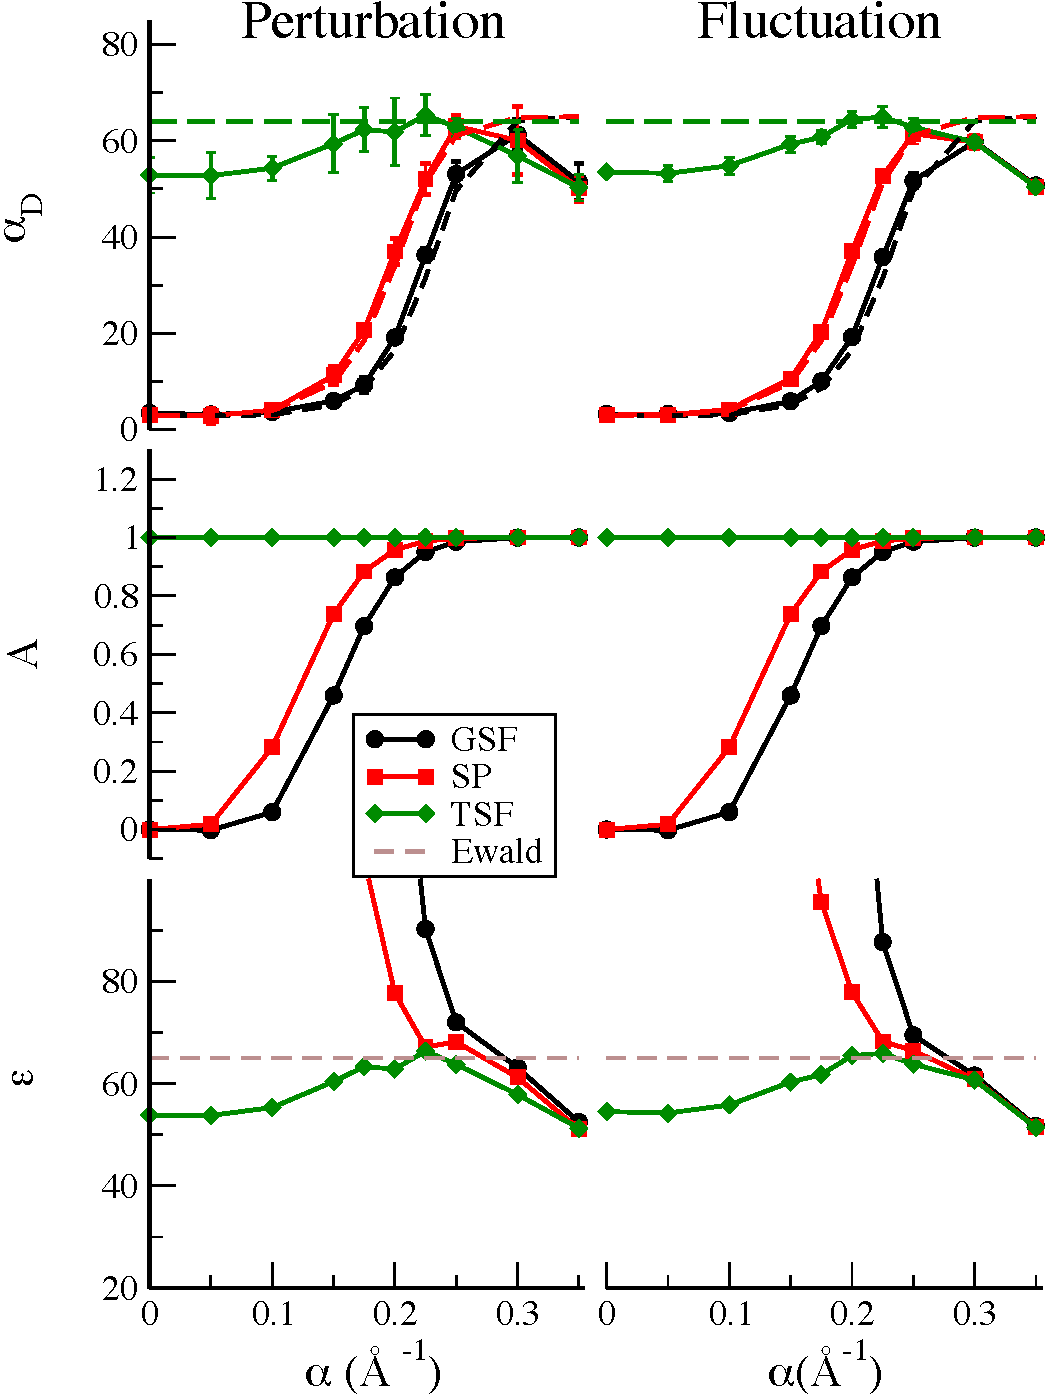
\includegraphics[width=4.5in]{dielectricFinal_Dipole.pdf}
\caption{The polarizability ($\alpha_D$), correction factor ($A$), and
  dielectric constant ($\epsilon$) for the test dipolar fluid. The
  left panels were computed using external fields, and those on the
  right are the result of equilibrium fluctuations.  In the GSF and SP
  methods, the corrections are large in with small values of $\alpha$,
  and a optimal damping coefficient is evident around 0.25 \AA$^{-1}$.
  The dashed lines in the upper panel indicate back-calculation of the
  polarizability using the Ewald estimate (Refs.\cite{Adams81}
  and \cite{NeumannI83}) for the dielectric constant.}
\label{fig:dielectricDipole}
\end{center}
\end{figure}
The macroscopic polarizability ($\alpha_D$) for the dipolar fluid is
shown in the upper panels in Fig. \ref{fig:dielectricDipole}.  The
polarizability obtained from the both perturbation and fluctuation
approaches are in excellent agreement with each other.  The data also
show a stong dependence on the damping parameter for both the Shifted
Potential (SP) and Gradient Shifted force (GSF) methods, while Taylor
shifted force (TSF) is largely independent of the damping
parameter.

The calculated correction factors discussed in section
\ref{sec:corrFactor} are shown in the middle panels. Because the TSF
method has $A = 1$ for all values of the damping parameter, the
computed polarizabilities need no correction for the dielectric
calculation. The value of $A$ varies with the damping parameter in
both the SP and GSF methods, and inclusion of the correction yields
dielectric estimates (shown in the lower panel) that are generally too
large until the damping reaches $\sim$~0.25~\AA$^{-1}$. Above this
value, the dielectric constants are generally in good agreement with
previous simulation results.\cite{NeumannI83}

Fig.~\ref{fig:dielectricDipole} also contains back-calculations of
the polarizability using the reference (Ewald) simulation
results.\cite{NeumannI83} These are indicated with dashed lines in the
upper panels.  It is clear that the expected polarizability for the SP
and GSF methods are quite close to results obtained from the
simulations.  This indicates that the correction formula for the
dipolar fluid (Eq.~(\ref{correctionFormula})) is quite sensitive when
the value of $\mathrm{A}$ deviates significantly from unity.

These results also suggest an optimal value for the damping parameter
of ($\alpha \sim 0.2-0.3$~\AA$^{-1}$) when evaluating dielectric
constants of point dipolar fluids using either the perturbation and
fluctuation approaches for the new real-space methods.

\begin{figure}
\begin{center}
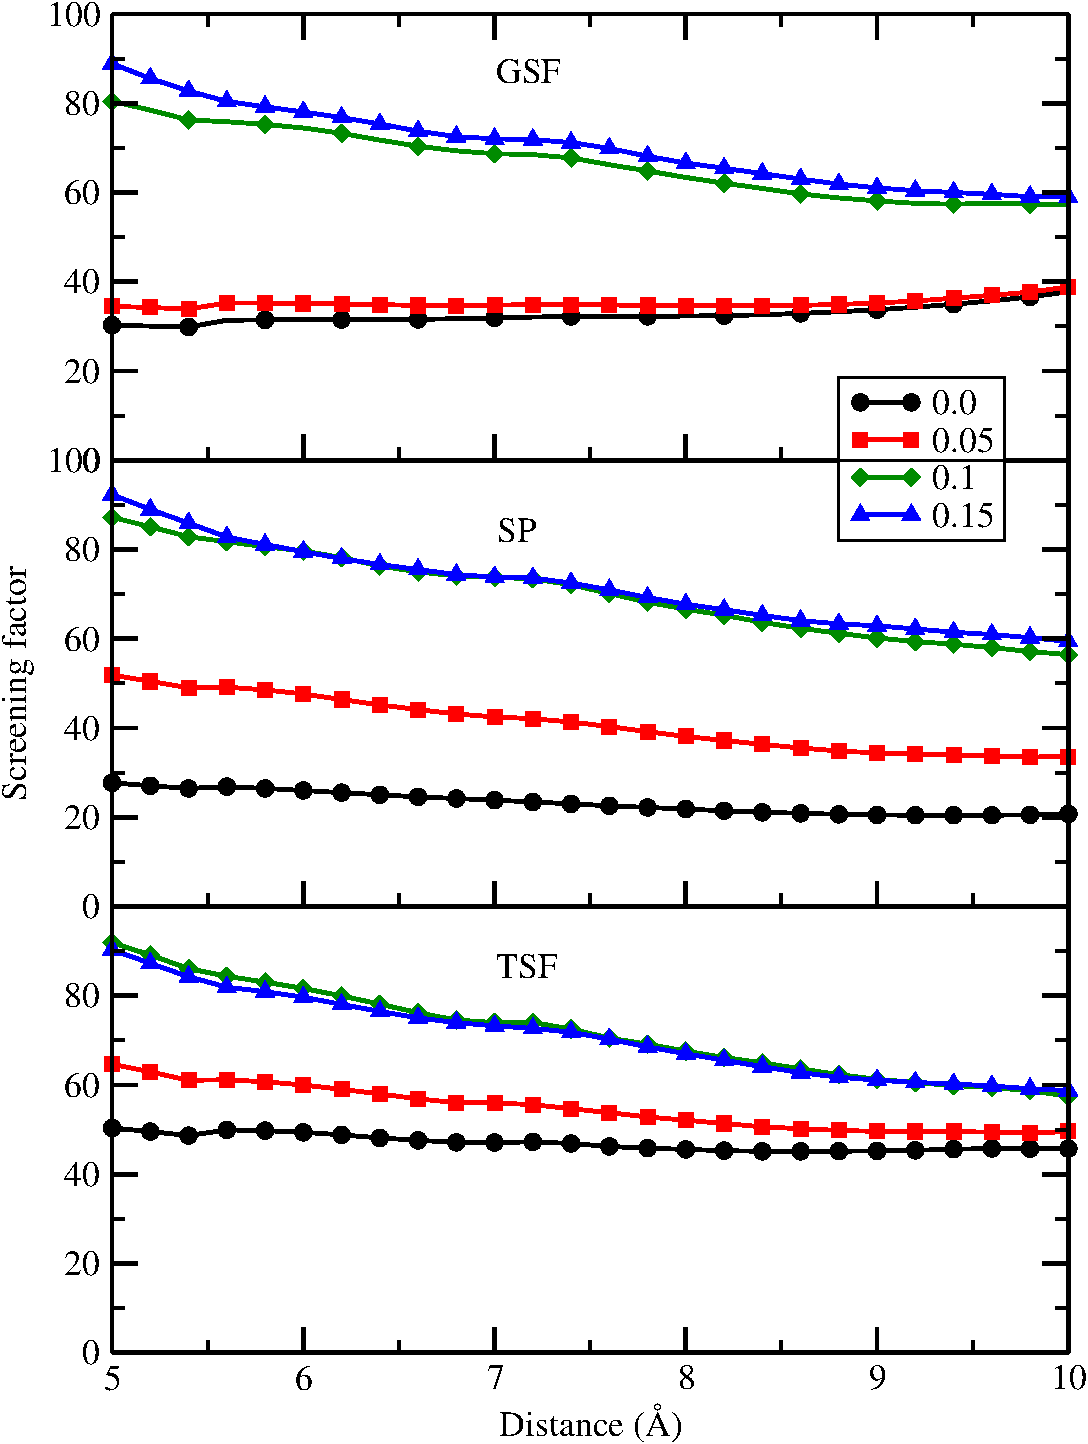
\includegraphics[width=4.5in]{ScreeningFactor_Dipole.pdf}
\caption{The distance-dependent screening factor, $\epsilon(r)$,
  between two ions immersed in the dipolar fluid. The new methods are
  shown in separate panels, and different values of the damping
  parameter ($\alpha$) are indicated with different symbols. All of
  the methods appear to be converging to the bulk dielectric constant
  ($\sim 65$) at large ion separations.}
\label{fig:ScreeningFactor_Dipole}
\end{center}
\end{figure}
We have also evaluated the distance-dependent screening factor,
$\epsilon(r)$, between two oppositely charged ions when they are
placed in the dipolar fluid.  These results were computed using
Eq.~(\ref{eq:pmf}) and are shown in Fig.
\ref{fig:ScreeningFactor_Dipole}.

The screening factor is similar to the dielectric constant, but
measures a local property of the ions in the fluid and depends on both
ion-dipole and dipole-dipole interactions. These interactions depend
on the distance between ions as well as the electrostatic interaction
methods utilized in the simulations. The screening should converge to
the dielectric constant when the field due to ions is small. This
occurs when the ions are separated (or when the damping parameter is
large). In Fig. \ref{fig:ScreeningFactor_Dipole} we observe that for
the higher value of damping alpha \textit{i.e.}
$\alpha = 0.2$~\AA$^{-1}$ and $0.3$~\AA$^{-1}$ and large separation
between ions, the screening factor does indeed approach the correct
dielectric constant.

It is also notable that the TSF method again displays smaller
perturbations away from the correct dielectric screening behavior.  We
also observe that for TSF method yields high dielectric screening even
for lower values of $\alpha$. 

At short distances, the presence of the ions creates a strong local
field that acts to align nearby dipoles nearly perfectly in opposition
to the field from the ions.  This has the effect of increasing the
effective screening when the ions are brought close to one another.
This effect is present even in the full Ewald treatment, and indicates
that the local ordering behavior is being captured by all of the
moderately-damped real-space methods.

\subsection{Quadrupolar fluid}
\begin{figure}
\begin{center}
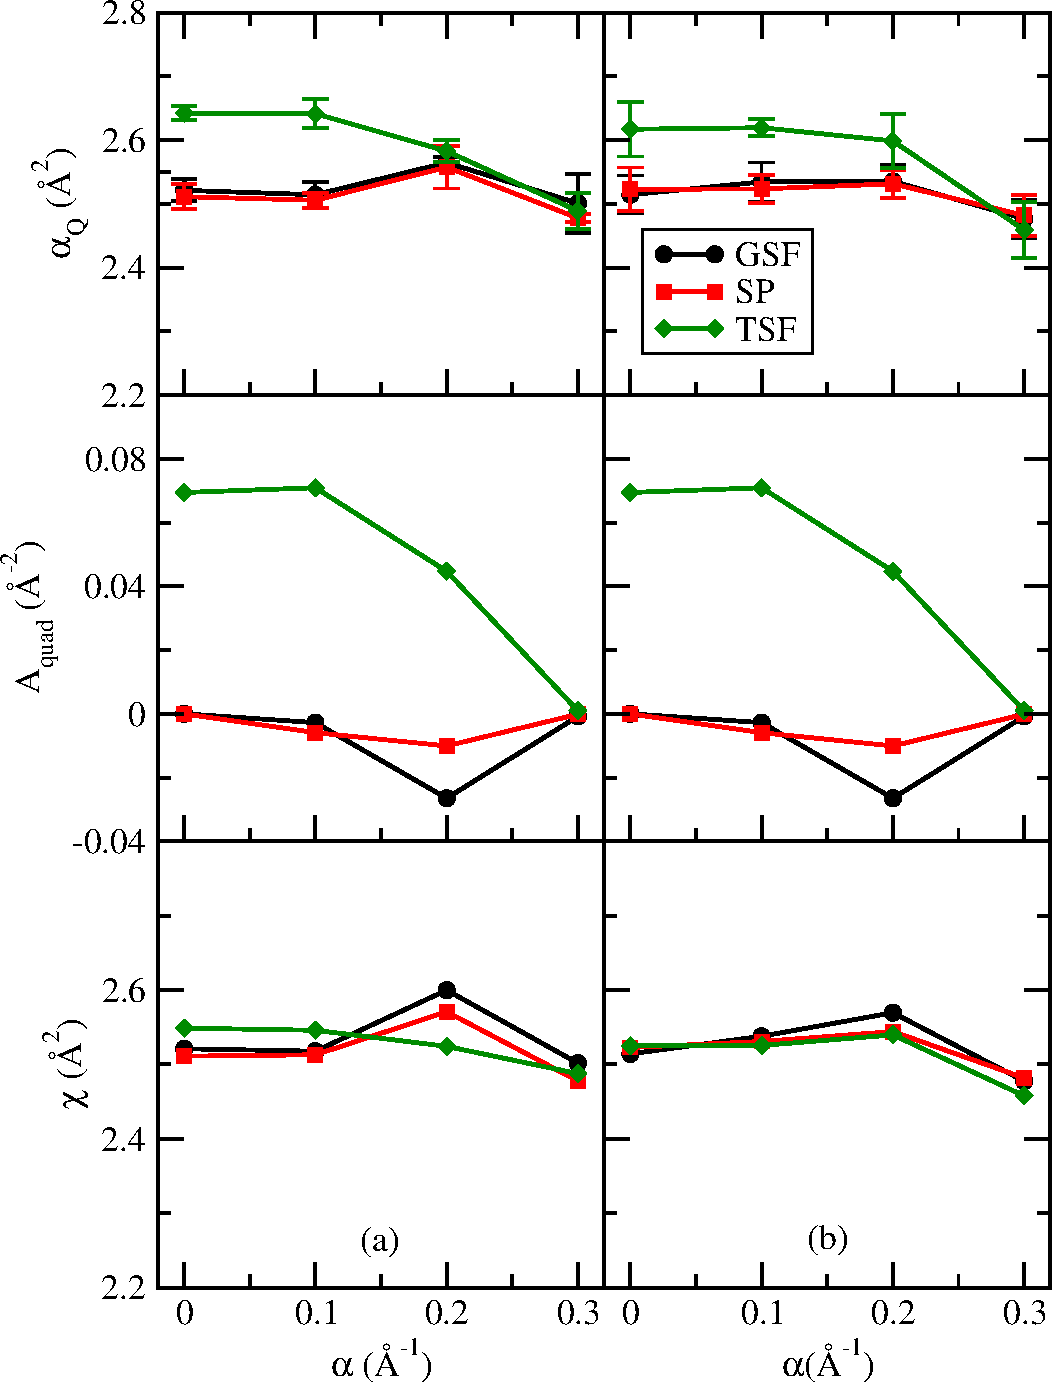
\includegraphics[width=4.5in]{polarizabilityFinal_Quad.pdf}
\caption{The quadrupole polarizability ($\alpha_Q$), correction factor
  ($B$), and susceptibility ($\chi_Q$) for the test quadrupolar
  fluid. The left panels were computed using external field gradients,
  and those on the right are the result of equilibrium fluctuations.
  The GSF and SP methods allow nearly unmodified use of the
  ``conducting boundary'' or polarizability results in place of the
  bulk susceptibility.}
\label{fig:dielectricQuad}
\end{center}
\end{figure}
The polarizability ($\alpha_Q$), correction factor ($B$), and
susceptibility ($\chi_Q$) for the quadrupolar fluid is plotted against
damping parameter Fig.  \ref{fig:dielectricQuad}.  In quadrupolar
fluids, both the polarizability and susceptibility have units of
$\mathrm{length}^2$. Although the susceptibility has dimensionality, it
is the relevant measure of macroscopic quadrupolar
properties.\cite{JeonI03, JeonII03} The left panel in
Fig. \ref{fig:dielectricQuad} shows results obtained from the applied
field gradient simulations whereas the results from the equilibrium
fluctuation formula are plotted in the right panels.

The susceptibility for the quadrupolar fluid is obtained from
quadrupolarizability and a correction factor using
Eq.~(\ref{eq:quadrupolarSusceptiblity}).  The susceptibilities are
shown in the bottom panels of Fig. \ref{fig:dielectricQuad}. All three
methods: (SP, GSF, and TSF) produce similar susceptibilities over the
range of damping parameters.  This shows that susceptibility derived
using the quadrupolarizability and the correction factors are
essentially independent of the electrostatic method utilized in the
simulation.

\begin{figure}
\begin{center}
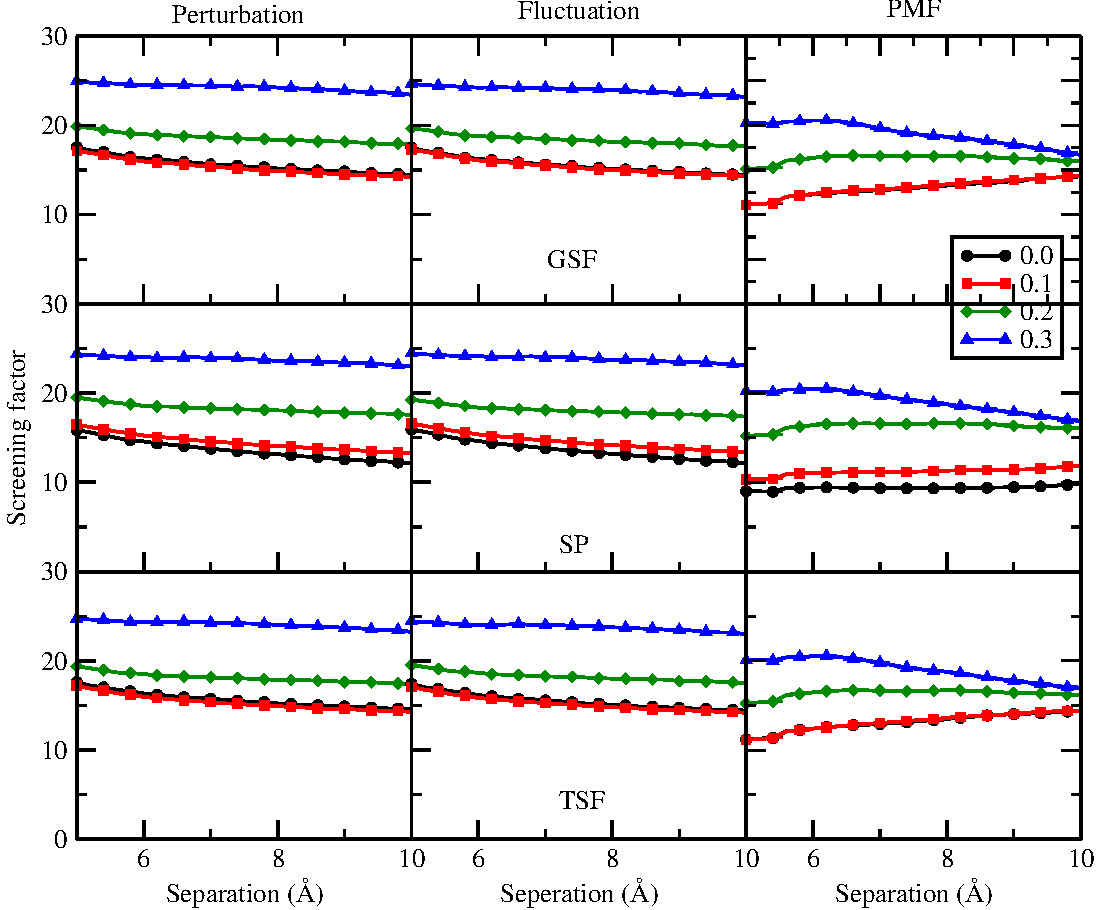
\includegraphics[width=\linewidth]{ScreeningFactor_Quad.pdf}
\caption{\label{fig:screenQuad} The distance-dependent screening
  factor, $\epsilon(r)$, between two ions immersed in the quadrupolar
  fluid. Results from  the perturbation and fluctuation methods are
  shown in right and central panels. Here the susceptibility is
  calculated from the  simulation and the geometrical factor is
  evaluated analytically, using the field and field-gradient produced
  by ions. The right hand panel shows the screening factor obtained
  from the PMF calculations.}
  \end{center}
\end{figure}
A more difficult test of the quadrupolar susceptibility is made by
comparing with direct calculation of the electrostatic screening using
the potential of mean force (PMF). Since the effective dielectric
constant for a quadrupolar fluid depends on the geometry of the field
and field gradient, this is not a physical property of the quadrupolar
fluid. 

The geometrical factor for embedded ions changes with the ion
separation distance. It is therefore reasonable to treat the
dielectric constant as a distance-dependent screening factor.  Since
the quadrupolar molecules couple with the gradient of the field, the
distribution of the quadrupoles will be inhomogeneously distributed
around the point charges.  Hence the distribution of quadrupolar
molecules should be taken into account when computing the geometrical
factors in the presence of this perturbation,
\begin{eqnarray}
G &=& \frac{\int_V g(\mathbf{r})  \left|\nabla \mathbf{E}^\circ
  \right|^2 d\mathbf{r}}{\int_V\left|\mathbf{E}^\circ\right|^2
  d\mathbf{r}}  \nonumber \\ \nonumber \\
 &=& \frac{ 2 \pi \int_{-1}^{1}  \int_{0}^{R} r^2  g(r,
     \cos\theta)  \left|\nabla \mathbf{E}^\circ  \right|^2 dr d(\cos\theta) }{\int_V\left|\mathbf{E}^\circ\right|^2 d\mathbf{r}}
\label{eq:geometricalFactor}
\end{eqnarray}
where $g(r,\cos\theta)$ is a distribution function for the quadrupoles
with respect to an origin at midpoint of a line joining the two probe
charges.

The effective screening factor is plotted against ion separation
distance in Fig. \ref{fig:screenQuad}.  The screening evaluated from
the perturbation and fluctuation methods are shown in right and
central panels. Here the susceptibility is calculated from the
simulation and the geometrical factor is evaluated analytically, using
the field and field-gradient produced by ions. The right hand panel
shows the screening factor obtained from the PMF calculations.

We note that the screening factor obtained from both the perturbation
and fluctuation formula show good agreement with the screening factor
calculated using PMF method. As there are no large differences in
quadrupole-quadruople interactions for various real-space
methods,\cite{PaperI,PaperII} we generally good agreement for the
screening factors using any of the real space methods.

\section{Summary}
We have used both perturbation and fluctuation approaches to evaluate
dielectric properties for dipolar and quadrupolar fluids.  The static
dielectric constant is the relevant bulk property for dipolar fluids,
while the quadrupolar susceptibility plays a similar role for
quadrupoles.  Corrections to both the static dielectric constant and
the quadrupolar susceptibility were derived for three new real space
electrostatic methods, and these corrections were tested against a
third measure of dielectric screening, the potential of mean force
between two ions immersed in the fluids.

For the dipolar fluids, we find that the polarizability evaluated
using the perturbation and fluctuation methods show excellent
agreement, indicating that equilibrium calculations of the dipole
fluctuations are good measures of bulk polarizability. One of the
findings of the Chapter 3 is that the moderately
damped GSF and SP methods were most suitable for molecular dynamics
and Monte Carlo simulations, respectively.\cite{PaperII}

The dielectric constant evaluated using the computed polarizability
and correction factors agrees well with the previous Ewald-based
simulation results \cite{Adams81,NeumannI83} for moderate damping
parameters in the range 0.25-0.3~\AA~$^{-1}$. 

Although the TSF method alters many dynamic and structural features in
multipolar liquids,\cite{PaperII} it is surprisingly good at computing
bulk dielectric properties at nearly all ranges of the damping
parameter.  In fact, the correction factor, $A = 1$, for the TSF
method so the conducting boundary formula is essentially correct when
using this method for point dipolar fluids.

The dielectric correction formula (Eq.~(\ref{correctionFormula}))
is extremely sensitive when the correction factor ($A$) deviates from
1, and this behavior is also seen in the effective screening of ions
embedded in the fluid. 

As in the dipolar case, the quadpole polarizability evaluated from
both perturbation and fluctuation simulations show excellent
agreement, again confirming that equilibrium fluctuation calculations
are sufficient to reproduce bulk dielectric properties in these
fluids.  The quadrupolar susceptibility calculated via our derived
correction factors tends to produce the same result for all three real
space methods.  Similarly, the screening factor calculated using the
susceptibility and a weighted geometric factor provides good agreement
with results obtained directly via potentials of mean force.  For
quadrupolar fluids, the distance dependence of the electrostatic
interaction is significantly reduced and the correction factors are
all small.  These points suggest that how an electrostatic method
treats the cutoff radius become less consequential for higher order
multipoles.
   
For this reason, we renew our recommendation that the
moderately-damped GSF method is an excellent choice for molecular
dynamics simulation where point-multipole interactions are being
utilized to compute bulk properties of fluids.

% % uncomment the following lines,
% if using chapter-wise bibliography
%
% \bibliographystyle{ndnatbib}
% \bibliography{example}


% Chapter 5

%
% Modified by Megan Patnott
% Last Change: Jan 18, 2013
%
%%%%%%%%%%%%%%%%%%%%%%%%%%%%%%%%%%%%%%%%%%%%%%%%%%%%%%%%%%%%%%%%%%%%%%%%
%
% Modified by Sameer Vijay
% Last Change: Tue Jul 26 2005 13:00 CEST
%
%%%%%%%%%%%%%%%%%%%%%%%%%%%%%%%%%%%%%%%%%%%%%%%%%%%%%%%%%%%%%%%%%%%%%%%%
%
% Sample Notre Dame Thesis/Dissertation
% Using Donald Peterson's ndthesis classfile
%
% Written by Jeff Squyres and Don Peterson
%
% Provided by the Information Technology Committee of
%   the Graduate Student Union
%   http://www.gsu.nd.edu/
%
% Nothing in this document is serious except the format.  :-)
%
% If you have any suggestions, comments, questions, please send e-mail
% to: ndthesis@gsu.nd.edu
%
%%%%%%%%%%%%%%%%%%%%%%%%%%%%%%%%%%%%%%%%%%%%%%%%%%%%%%%%%%%%%%%%%%%%%%%%


%
% Chapter 5
%

\chapter{CONCLUSIONS}
In this dissertation, I have presented the three newly developed real-space methods: Shifted Potential (SP), Gradient Shifted Force (GSF), and Taylor Shifted Force (TSF), for evaluating electrostatic interactions between multipoles in molecular simulations. I have also computed various static and dynamic properties using newly developed real space methods and compared result with the Ewald sum. I have also studied the conservation of total energy using real-space as well as Ewald method. Finally, I have discussed the perturbation, fluctuation, and PMF methods for calculating dielectric properties for dipolar and quadrupolar systems.

The energy constant evaluated for the dipolar and quadrupolar crystal using SP and GSF methods show excellent agreement with the analytical result. The TSF method performs poorly in predicting the energy constant for both dipolar and quadrupolar crystal. We need to take larger cutoff radius and suitable damping alpha to predict energy constant using TSF method. For the dipolar crystal, higher damping favors the quick convergence of the energy constant when plotted against cutoff radius. But the higher damping can presents additional issues while calculating energy constant for quadrupolar crystal, hence the small damping parameter is suitable for the quadrupolar system.     

The SP method is the mutipolar version of the Wolf's shifted potential for the charge-charge interaction, whereas the GSF and TSF method are multipolar generalization of the Damped Shifted Force (DSF) method. In the SP method, the potential energy smoothly approaches to zero at the cutoff radius but the forces and torques derived from the energies are not continuous at the cutoff radius. On the other hand, the forces and torques as well as energies evaluated in the GSF and TSF method vanishes at the cutoff radius. Since the energy evaluated from the SP method shows excellent agreement with the Ewald, it is suitable for the Monte Carlo (MC) simulation. The GSF method performs well in conserving total energy in MD simulations and produces good quantitative agreement with the Ewald energies, forces and torques, therefore better choice for MD simulations. Both SP and GSF models perform remarkably well with moderate damping parameter for reproducing static as well as dynamic properties in the liquid systems. All of these real-space methods scales \textit{linearly} with system size and are easily parallelizable, therefore reduce computational cost substantially while performing large simulations.         

The test of the dielectric properties is very important to validate the electrostatic interaction methods. I presented three methods: perturbation, fluctuation, and potential of mean force (PMF), to evaluate dielectric properties for dipolar and quadrupolar fluids. The polarizability obtained from simulations, using perturbation and fluctuation methods, shows excellent agreement with each other for all SP, GSF, and TSF methods. To calculate the dielectric constant and susceptibility from the dipolar polarization (measured from simulations), we need to take account of correction factor listed in the Chapter 4. The correction factor for TSF method is 1, which essentially signifies no correction. Therefore the dielectric constant evaluated using conducting boundary condition can produce good result for all values of damping alpha. In the other words, the susceptibility and polarizability are the same in the case of dipolar TSF method. The correction factor for SP and GSF methods depend on damping parameter as well as cutoff radius. The formula for deriving dielectric constant from polarization is very sensitive when the damping parameter is very small. Therefore moderate damping alpha between ($0.25 - 0.3~\AA^{-2}$) are always suitable choice for calculating dielectric properties using SP and GSF method.

For the quadrupolar fluid, the correction factor essentially small for SP and GSF method whereas the correction factor is comparatively large for the TSF. Different than dipolar case, the quadrupolar susceptibility but not dielectric screening measures the actual bulk properties of the quadrupolar fluid. On other hand, the dielectric constant is geometry dependent and can be derived from the susceptibility and geometry of the applied field. 

The dipolar dielectric screening calculated from the perturbation and fluctuation also agree with the screening factor measured from the PMF method for the damping parameter $0.25 - 0.3~\AA^{-2}$. Similarly the quadrupolar dielectric screening calculated between two point charges using susceptibility and geometrical factor shows good agreement with the direct screening measured using PMF method.

All of these newly developed real space methods are computationally very efficient as compared to Ewald method. The physical properties predicted by the real-space methods, with the suitable choice of damping parameter, are as accurate as the computationally expensive Ewald method. We can even predict the dielectric properties correctly using newly developed methods with the use of the correction factor. Therefore our newly developed real space methods are the suitable choice for calculating electrostatic interactions between molecules in the large molecular simulations.         
    

  



% % uncomment the following lines,
% if using chapter-wise bibliography
%
% \bibliographystyle{ndnatbib}
% \bibliography{example}
% Appendix (optional)

\appendix

%
% Modified by Sameer Vijay
% Last Change: Wed Jul 27 2005 13:00 CEST
%
%%%%%%%%%%%%%%%%%%%%%%%%%%%%%%%%%%%%%%%%%%%%%%%%%%%%%%%%%%%%%%%%%%%%%%%%
%
% Sample Notre Dame Thesis/Dissertation
% Using Donald Peterson's ndthesis classfile
%
% Written by Jeff Squyres and Don Peterson
%
% Provided by the Information Technology Committee of
%   the Graduate Student Union
%   http://www.gsu.nd.edu/
%
% Nothing in this document is serious except the format.  :-)
%
% If you have any suggestions, comments, questions, please send e-mail
% to: ndthesis@gsu.nd.edu
%
%%%%%%%%%%%%%%%%%%%%%%%%%%%%%%%%%%%%%%%%%%%%%%%%%%%%%%%%%%%%%%%%%%%%%%%%

%%%%%%%%%%%%%%%%%%%%%%%%%%%%%%%%%%%%%%%%%%%%%%%%%%%%%%%%%%%%%%%%%%%%%%%%
%
% Appendix
%
%%%%%%%%%%%%%%%%%%%%%%%%%%%%%%%%%%%%%%%%%%%%%%%%%%%%%%%%%%%%%%%%%%%%%%%%

\chapter{RADIAL FUNCTIONS FOR REAL-SPACE ELECTROSTATIC METHODS}

\section{Smith's $B_l(r)$ functions for damped-charge distributions}
\label{SmithFunc}
The following summarizes Smith's $B_l(r)$ functions and includes
formulas given in his appendix.\cite{Smith98} The first function
$B_0(r)$ is defined by
%
\begin{equation}
B_0(r)=\frac{\text{erfc}(\alpha r)}{r} = \frac{2}{\sqrt{\pi}r}
\int_{\alpha r}^{\infty} \text{e}^{-s^2} ds .
\end{equation}
%
The first derivative of this function is
%
\begin{equation}
\frac{dB_0(r)}{dr}=-\frac{1}{r^2}\text{erfc}(\alpha r)
-\frac{2\alpha}{r\sqrt{\pi}}\text{e}^{-{\alpha}^2r^2}
\end{equation}
%
which can be used to define a function $B_1(r)$:
%
\begin{equation}
B_1(r)=-\frac{1}{r}\frac{dB_0(r)}{dr}
\end{equation}
%
In general, the recurrence relation,
\begin{equation}
B_l(r)=-\frac{1}{r}\frac{dB_{l-1}(r)}{dr} 
= \frac{1}{r^2} \left[ (2l-1)B_{l-1}(r) + \frac {(2\alpha^2)^l}{\alpha \sqrt{\pi}}
\text{e}^{-{\alpha}^2r^2}
\right] ,
\end{equation}
is very useful for building up higher derivatives. As noted by Smith,
it is possible to approximate the $B_l(r)$ functions,
%
\begin{equation}
B_l(r)=\frac{(2l)!}{l!2^lr^{2l+1}} - \frac {(2\alpha^2)^{l+1}}{(2l+1)\alpha \sqrt{\pi}}
+\text{O}(r) .
\end{equation}

\newpage
\section{The $r$-dependent factors for TSF electrostatics}
\label{radialTSF}

Using the shifted damped functions $f_n(r)$ defined by:
%
\begin{equation}
f_n(r)= B_0(r) -\sum_{m=0}^{n+1} \frac {(r-r_c)^m}{m!} B_0^{(m)}(r_c)  ,
\end{equation}
%
where the superscript $(m)$ denotes the $m^\mathrm{th}$ derivative. In
this Appendix, we provide formulas for successive derivatives of this
function.  (If there is no damping, then $B_0(r)$ is replaced by
$1/r$.)  First, we find:
%
\begin{equation}
\frac{\partial f_n}{\partial r_\alpha}=\hat{r}_\alpha \frac{d f_n}{d r} .
\end{equation}
%
This formula clearly brings in derivatives of Smith's $B_0(r)$
function, and we define higher-order derivatives as follows:
%
\begin{align}
g_n(r)=& \frac{d f_n}{d r} =
B_0^{(1)}(r) -\sum_{m=0}^{n} \frac {(r-r_c)^m}{m!} B_0^{(m+1)}(r_c) \\
h_n(r)=& \frac{d^2f_n}{d r^2} =
B_0^{(2)}(r) -\sum_{m=0}^{n-1} \frac {(r-r_c)^m}{m!} B_0^{(m+2)}(r_c) \\
s_n(r)=& \frac{d^3f_n}{d r^3} =
B_0^{(3)}(r) -\sum_{m=0}^{n-2} \frac {(r-r_c)^m}{m!} B_0^{(m+3)}(r_c) \\
t_n(r)=& \frac{d^4f_n}{d r^4} =
B_0^{(4)}(r) -\sum_{m=0}^{n-3} \frac {(r-r_c)^m}{m!} B_0^{(m+4)}(r_c) \\
u_n(r)=& \frac{d^5f_n}{d r^5} =
B_0^{(5)}(r) -\sum_{m=0}^{n-4} \frac {(r-r_c)^m}{m!} B_0^{(m+5)}(r_c)  .
\end{align}
%
We note that the last function needed (for quadrupole-quadrupole interactions) is
%
\begin{equation}
u_4(r)=B_0^{(5)}(r) - B_0^{(5)}(r_c) .
\end{equation}
% The functions
% needed are listed schematically below:
% %
% \begin{eqnarray}
% f_0 \quad f_1 \qquad \qquad \quad & \nonumber \\
% g_0 \quad g_1 \quad g_2 \quad g_3 \quad &g_4 \nonumber \\
% h_1 \quad h_2 \quad h_3 \quad &h_4 \nonumber \\
% s_2 \quad s_3 \quad &s_4 \nonumber \\
% t_3 \quad &t_4 \nonumber \\
% &u_4 \nonumber .
% \end{eqnarray}
The functions $f_n(r)$ to $u_n(r)$ can be computed recursively and
stored on a grid for values of $r$ from $0$ to $r_c$.  Using these
functions, we find
%
\begin{align}
\frac{\partial f_n}{\partial r_\alpha} =&r_\alpha \frac {g_n}{r} \label{eq:b9}\\
\frac{\partial^2 f_n}{\partial r_\alpha \partial r_\beta} =&\delta_{\alpha \beta}\frac {g_n}{r} 
+r_\alpha r_\beta \left( -\frac{g_n}{r^3} +\frac{h_n}{r^2}\right) \\
\frac{\partial^3 f_n}{\partial r_\alpha \partial r_\beta \partial r_\gamma} =&
\left( \delta_{\alpha \beta} r_\gamma + \delta_{\alpha \gamma} r_\beta + 
\delta_{ \beta \gamma} r_\alpha \right)  
\left(  -\frac{g_n}{r^3} +\frac{h_n}{r^2} \right) \nonumber \\
& + r_\alpha r_\beta r_\gamma 
\left(  \frac{3g_n}{r^5}-\frac{3h_n}{r^4} +\frac{s_n}{r^3} \right) \\
\frac{\partial^4 f_n}{\partial r_\alpha \partial r_\beta \partial
  r_\gamma \partial r_\delta} =& 
\left( \delta_{\alpha \beta} \delta_{\gamma \delta} 
+ \delta_{\alpha \gamma} \delta_{\beta \delta}
 +\delta_{ \beta \gamma} \delta_{\alpha \delta} \right)
\left( - \frac{g_n}{r^3} + \frac{h_n}{r^2} \right)  \nonumber \\ 
&+ \left( \delta_{\alpha \beta} r_\gamma r_\delta
+ \text{5 permutations}
\right) \left( \frac{3 g_n}{r^5} - \frac{3h_n}{r^4} + \frac{s_n}{r^3} 
\right) \nonumber \\
&+ r_\alpha r_\beta r_\gamma r_\delta
\left(  -\frac{15g_n}{r^7} + \frac{15h_n}{r^6} - \frac{6s_n}{r^5}
+ \frac{t_n}{r^4} \right)\\
\frac{\partial^5 f_n}
{\partial r_\alpha \partial r_\beta \partial r_\gamma \partial
  r_\delta \partial r_\epsilon} =& 
\left( \delta_{\alpha \beta} \delta_{\gamma \delta} r_\epsilon
+ \text{14 permutations} \right) 
\left(  \frac{3g_n}{r^5}-\frac{3h_n}{r^4} +\frac{s_n}{r^3} \right) \nonumber \\
&+ \left( \delta_{\alpha \beta} r_\gamma r_\delta r_\epsilon
+ \text{9 permutations}
\right) \left(- \frac{15g_n}{r^7}+\frac{15h_n}{r^7} -\frac{6s_n}{r^5} +\frac{t_n}{r^4} 
\right) \nonumber \\
&+ r_\alpha r_\beta r_\gamma r_\delta r_\epsilon
\left(  \frac{105g_n}{r^9} - \frac{105h_n}{r^8} + \frac{45s_n}{r^7}
- \frac{10t_n}{r^6} +\frac{u_n}{r^5} \right) \label{eq:b13}
\end{align}
%
%
%
\newpage
\section{The $r$-dependent factors for GSF electrostatics}
\label{radialGSF}

In Gradient-shifted force electrostatics, the kernel is not expanded,
and the expansion is carried out on the individual terms in the
multipole interaction energies. For damped charges, this still brings
multiple derivatives of the Smith's $B_0(r)$ function into the
algebra. To denote these terms, we generalize the notation of the
previous appendix. For either $f(r)=1/r$ (undamped) or $f(r)=B_0(r)$
(damped),
%
\begin{align}
g(r) &= \frac{df}{d r} &&                      &&=-\frac{1}{r^2}
&&\mathrm{or~~~} -rB_1(r) \\
h(r) &= \frac{dg}{d r} &&= \frac{d^2f}{d r^2} &&= \frac{2}{r^3} &&\mathrm{or~~~}-B_1(r) + r^2 B_2(r) \\
s(r) &= \frac{dh}{d r} &&= \frac{d^3f}{d r^3} &&=-\frac{6}{r^4}&&\mathrm{or~~~}3rB_2(r) - r^3 B_3(r)\\
t(r) &= \frac{ds}{d r} &&= \frac{d^4f}{d r^4} &&= \frac{24}{r^5} &&\mathrm{or~~~} 3
B_2(r) - 6r^2 B_3(r) + r^4 B_4(r) \\
u(r) &= \frac{dt}{d r} &&= \frac{d^5f}{d r^5} &&=-\frac{120}{r^6} &&\mathrm{or~~~} -15
r B_3(r) + 10 r^3B_4(r) -r^5B_5(r).
\end{align}
%
For undamped charges, Table I lists these derivatives under the Bare
Coulomb column. Equations \ref{eq:b9} to \ref{eq:b13} are still
correct for GSF electrostatics if the subscript $n$ is eliminated.

% % uncomment the following lines,
% if using chapter-wise bibliography
%
% \bibliographystyle{ndnatbib}
% \bibliography{example}
%
% Back stuff
%
% Modified by Sameer Vijay
% Last Change: Wed Jul 27 2005 13:00 CEST
%
%%%%%%%%%%%%%%%%%%%%%%%%%%%%%%%%%%%%%%%%%%%%%%%%%%%%%%%%%%%%%%%%%%%%%%%%
%
% Sample Notre Dame Thesis/Dissertation
% Using Donald Peterson's ndthesis classfile
%
% Written by Jeff Squyres and Don Peterson
%
% Provided by the Information Technology Committee of
%   the Graduate Student Union
%   http://www.gsu.nd.edu/
%
% Nothing in this document is serious except the format.  :-)
%
% If you have any suggestions, comments, questions, please send e-mail
% to: ndthesis@gsu.nd.edu
%
%%%%%%%%%%%%%%%%%%%%%%%%%%%%%%%%%%%%%%%%%%%%%%%%%%%%%%%%%%%%%%%%%%%%%%%%

%%%%%%%%%%%%%%%%%%%%%%%%%%%%%%%%%%%%%%%%%%%%%%%%%%%%%%%%%%%%%%%%%%%%%%%%
%
% Appendix
%
%%%%%%%%%%%%%%%%%%%%%%%%%%%%%%%%%%%%%%%%%%%%%%%%%%%%%%%%%%%%%%%%%%%%%%%%

\chapter{POINT MULTIPOLES, FIELD, AND FIELD GRADIENT }

\section{Point-multipolar interactions with a spatially-varying electric field}

We can treat objects $a$, $b$, and $c$ containing embedded collections
of charges. When we define the primitive moments, we sum over that
collections of charges using a local coordinate system within each
object.  The point charge, dipole, and quadrupole for object $a$ are
given by $C_a$, $\mathbf{D}_a$, and $\mathsf{Q}_a$, respectively.
These are the primitive multipoles which can be expressed as a
distribution of charges,
\begin{align}
C_a =&\sum_{k \, \text{in }a} q_k , \label{eq:charge} \\
D_{a\alpha} =&\sum_{k \, \text{in }a} q_k r_{k\alpha}, \label{eq:dipole}\\
Q_{a\alpha\beta} =& \frac{1}{2} \sum_{k \, \text{in }  a} q_k
r_{k\alpha}  r_{k\beta} . \label{eq:quadrupole}
\end{align}
Note that the definition of the primitive quadrupole here differs from
the standard traceless form, and contains an additional Taylor-series
based factor of $1/2$.  In Paper 1, we derived the forces and torques
each object exerts on the others.

Here we must also consider an external electric field that varies in
space: $\mathbf E(\mathbf r)$.  Each of the local charges $q_k$ in
object $a$ will then experience a slightly different field.  This
electric field can be expanded in a Taylor series around the local
origin of each object.  A different Taylor series expansion is carried
out for each object.

For a particular charge $q_k$, the electric field at that site's
position is given by:
\begin{equation}
E_\gamma + \nabla_\delta E_\gamma r_{k \delta} 
+ \frac {1}{2} \nabla_\delta \nabla_\varepsilon E_\gamma r_{k \delta}
r_{k \varepsilon} + ... 
\end{equation}
Note that the electric field is always evaluated at the origin of the
objects, and treating each object using point multipoles simplifies
this greatly.

To find the force exerted on object $a$ by the electric field, one
takes the electric field expression, and multiplies it by $q_k$, and
then sum over all charges in $a$:

\begin{align}
F_\gamma &=  \sum_{k \textrm{~in~} a} q_k \lbrace E_\gamma + \nabla_\delta E_\gamma r_{k \delta} 
+ \frac {1}{2} \nabla_\delta \nabla_\varepsilon E_\gamma r_{k \delta}
r_{k \varepsilon} + ...  \rbrace  \\
 &= C_a E_\gamma + D_{a  \delta} \nabla_\delta E_\gamma 
+ Q_{a \delta \varepsilon} \nabla_\delta \nabla_\varepsilon E_\gamma +
... 
\end{align}

Similarly, the torque exerted by the field on $a$ can be expressed as
\begin{align}
\tau_\alpha &=  \sum_{k \textrm{~in~} a} (\mathbf r_k \times q_k \mathbf E)_\alpha \\
 & =  \sum_{k \textrm{~in~} a} \epsilon_{\alpha \beta \gamma} q_k
 r_{k\beta} E_\gamma(\mathbf r_k) \\
 & = \epsilon_{\alpha \beta \gamma} D_\beta E_\gamma 
+ 2 \epsilon_{\alpha \beta \gamma} Q_{\beta \delta} \nabla_\delta
E_\gamma + ...
\end{align}

The last term is essentially identical with form derived by Torres del
Castillo and M\'{e}ndez Garrido,\cite{Torres-del-Castillo:2006uo} although their derivation
utilized a traceless form of the quadrupole that is different than the
primitive definition in use here.  We note that the Levi-Civita symbol
can be eliminated by utilizing the matrix cross product in an
identical form as in Ref. \onlinecite{Smith98}:
\begin{equation}
\left[\mathsf{A} \times \mathsf{B}\right]_\alpha = \sum_\beta
\left[\mathsf{A}_{\alpha+1,\beta} \mathsf{B}_{\alpha+2,\beta}
  -\mathsf{A}_{\alpha+2,\beta} \mathsf{B}_{\alpha+1,\beta} 
\right]
\label{eq:matrixCross}
\end{equation}
where $\alpha+1$ and $\alpha+2$ are regarded as cyclic permuations of
the matrix indices.  In table \ref{tab:UFT} we give compact
expressions for how the multipole sites interact with an external
field that has exhibits spatial variations.

\begin{table}
\caption{Potential energy $(U)$, force $(\mathbf{F})$, and torque
  $(\mathbf{\tau})$ expressions for a multipolar site embedded in an
  electric field with spatial variations, $\mathbf{E}(\mathbf{r})$.
\label{tab:UFT}}
\centering
\begin{tabular}{r|ccc}
  & Charge & Dipole & Quadrupole \\ \hline
$U$ &  $C \phi(\mathbf{r})$ & $-\mathbf{D} \cdot \mathbf{E}(\mathbf{r})$ & $- \mathsf{Q}:\nabla \mathbf{E}(\mathbf{r})$ \\
$\mathbf{F}$ & $C \mathbf{E}(\mathbf{r})$ & $+\mathbf{D} \cdot \nabla \mathbf{E}(\mathbf{r})$ &  $+\mathsf{Q} : \nabla\nabla\mathbf{E}(\mathbf{r})$ \\
$\mathbf{\tau}$ & & $\mathbf{D} \times \mathbf{E}(\mathbf{r})$ & $+2 \mathsf{Q} \times \nabla \mathbf{E}(\mathbf{r})$
\end{tabular}
\end{table}

\newpage

\section{Gradient of the field due to quadrupolar polarization}
\label{singularQuad}
In this section, we will discuss the gradient of the field produced by
quadrupolar polarization. For this purpose, we consider a distribution
of charge ${\rho}(r)$ which gives rise to an electric field
$\vec{E}(r)$ and gradient of the field $\vec{\nabla} \vec{E}(r)$
throughout space. The total gradient of the electric field over volume
due to the all charges within the sphere of radius $R$ is given by
(cf. Jackson equation 4.14):
\begin{equation}
\int_{r<R} \vec{\nabla}\vec{E}\;d^3r = -\int_{r=R} R^2 \vec{E}\;\hat{n}\; d\Omega
\label{eq:8}
\end{equation}
where $d\Omega$ is the solid angle and $\hat{n}$ is the normal vector
of the surface of the sphere which is equal to
$sin[\theta]cos[\phi]\hat{x} + sin[\theta]sin[\phi]\hat{y} +
cos[\theta]\hat{z}$
in spherical coordinates.  For the charge density ${\rho}(r')$, the
total gradient of the electric field can be written as (cf. Jackson
equation 4.16),
\begin{equation}
\int_{r<R} \vec{\nabla}\vec{E}\; d^3r=-\int_{r=R} R^2\; \vec{\nabla}\Phi\; \hat{n}\; d\Omega  =-\frac{1}{4\pi\;\epsilon_o}\int_{r=R} R^2\; \vec{\nabla}\;\left(\int \frac{\rho(r')}{|\vec{r}-\vec{r'}|}\;d^3r'\right) \hat{n}\; d\Omega
\label{eq:9}
\end{equation}
The radial function in the equation (\ref{eq:9}) can be expressed in
terms of spherical harmonics as (cf. Jackson equation 3.70),
\begin{equation}
\frac{1}{|\vec{r} - \vec{r'}|} = 4\pi \sum_{l=0}^{\infty}\sum_{m=-l}^{m=l}\frac{1}{2l+1}\;\frac{{r^l_<}}{{r^{l+1}_>}}\;{Y^*}_{lm}(\theta', \phi')\;Y_{lm}(\theta, \phi)
\label{eq:10}
\end{equation}
If the sphere completely encloses the charge density then $ r_< = r'$ and $r_> = R$. Substituting equation (\ref{eq:10}) into (\ref{eq:9}) we get,
\begin{equation}
\begin{split}
\int_{r<R} \vec{\nabla}\vec{E}\;d^3r &=-\frac{R^2}{\epsilon_o}\int_{r=R} \; \vec{\nabla}\;\left(\int \rho(r')\sum_{l=0}^{\infty}\sum_{m=-l}^{m=l}\frac{1}{2l+1}\;\frac{{r'^l}}{{R^{l+1}}}\;{Y^*}_{lm}(\theta', \phi')\;Y_{lm}(\theta, \phi)\;d^3r'\right) \hat{n}\; d\Omega \\
 &= -\frac{R^2}{\epsilon_o}\sum_{l=0}^{\infty}\sum_{m=-l}^{m=l}\frac{1}{2l+1}\;\int \rho(r')\;{r'^l}\;{Y^*}_{lm}(\theta', \phi')\left(\int_{r=R}\vec{\nabla}\left({R^{-(l+1)}}\;Y_{lm}(\theta, \phi)\right)\hat{n}\; d\Omega \right)d^3r
'
\end{split}
\label{eq:11}
\end{equation} 
The gradient of the product of radial function and spherical harmonics
is given by (cf. Arfken, p.811 eq. 16.94):
\begin{equation}
\begin{split}
\vec{\nabla}\left[ f(r)\;Y_{lm}(\theta, \phi)\right] = &-\left(\frac{l+1}{2l+1}\right)^{1/2}\; \left[\frac{\partial}{\partial r}-\frac{l}{r} \right]f(r)\; Y_{l, l+1, m}(\theta, \phi)\\ &+ \left(\frac{l}{2l+1}\right)^{1/2}\left[\frac
{\partial}{\partial r}+\frac{l}{r} \right]f(r)\; Y_{l, l-1, m}(\theta, \phi).
\end{split}
\label{eq:12}
\end{equation}
Using equation (\ref{eq:12}) we get,
\begin{equation}
\vec{\nabla}\left({R^{-(l+1)}}\;Y_{lm}(\theta, \phi)\right) = [(l+1)(2l+1)]^{1/2}\; Y_{l,l+1,m}(\theta, \phi) \; \frac{1}{R^{l+2}},
\label{eq:13}
\end{equation}
where $ Y_{l,l+1,m}(\theta, \phi)$ is the vector spherical harmonics
which can be expressed in terms of spherical harmonics as shown in
below (cf. Arfkan p.811),
\begin{equation}
Y_{l,l+1,m}(\theta, \phi) = \sum_{m_1, m_2} C(l+1,1,l|m_1,m_2,m)\; {Y_{l+1}}^{m_1}(\theta,\phi)\; \hat{e}_{m_2},
\label{eq:14}
\end{equation}
where $C(l+1,1,l|m_1,m_2,m)$ is a Clebsch-Gordan coefficient and
$\hat{e}_{m_2}$ is a spherical tensor of rank 1 which can be expressed
in terms of Cartesian coordinates,
\begin{equation}
{\hat{e}}_{+1} = - \frac{\hat{x}+i\hat{y}}{\sqrt{2}},\quad {\hat{e}}_{0} = \hat{z},\quad and \quad {\hat{e}}_{-1} = \frac{\hat{x}-i\hat{y}}{\sqrt{2}}
\label{eq:15}
\end{equation} 
The normal vector $\hat{n} $ can be expressed in terms of spherical tensor of rank 1 as shown in below,
\begin{equation}
\hat{n} = \sqrt{\frac{4\pi}{3}}\left(-{Y_1}^{-1}{\hat{e}}_1 -{Y_1}^{1}{\hat{e}}_{-1} + {Y_1}^{0}{\hat{e}}_0 \right)
\label{eq:16}
\end{equation}
The surface integral of the product of $\hat{n}$ and
${Y_{l+1}}^{m_1}(\theta, \phi)$ gives,
\begin{equation}
\begin{split}
\int \hat{n}\;{Y_{l+1}}^{m_1}\;d\Omega &= \int \sqrt{\frac{4\pi}{3}}\left(-{Y_1}^{-1}{\hat{e}}_1 -{Y_1}^{1}{\hat{e}}_{-1} + {Y_1}^{0}{\hat{e}}_0 \right)\;{Y_{l+1}}^{m_1}\; d\Omega \\
&=  \int \sqrt{\frac{4\pi}{3}}\left({{Y_1}^{1}}^* {\hat{e}}_1 +{{Y_1}^{-1}}^* {\hat{e}}_{-1} + {{Y_1}^{0}}^* {\hat{e}}_0 \right)\;{Y_{l+1}}^{m_1}\; d\Omega \\
&=   \sqrt{\frac{4\pi}{3}}\left({\delta}_{l+1, 1}\;{\delta}_{1, m_1}\;{\hat{e}}_1 + {\delta}_{l+1, 1}\;{\delta}_{-1, m_1}\;{\hat{e}}_{-1}+ {\delta}_{l+1, 1}\;{\delta}_{0, m_1} \;{\hat{e}}_0\right),
\end{split}
\label{eq:17}
\end{equation}
where ${Y_{l}}^{-m} = (-1)^m\;{{Y_{l}}^{m}}^* $ and
$ \int {{Y_{l}}^{m}}^*\;{Y_{l'}}^{m'}\;d\Omega =
\delta_{ll'}\delta_{mm'} $.
Non-vanishing values of equation \ref{eq:17} require $l = 0$,
therefore the value of $ m = 0 $. Since the values of $ m_1$ are -1,
1, and 0 then $m_2$ takes the values 1, -1, and 0, respectively
provided that $m = m_1 + m_2$.  Equation \ref{eq:11} can therefore be
modified,
\begin{equation}
\begin{split}
\int_{r<R} \vec{\nabla}\vec{E}\;d^3r = &- \sqrt{\frac{4\pi}{{3}}}\;\frac{1}{\epsilon_o}\int \rho(r')\;{Y^*}_{00}(\theta', \phi')[ C(1, 1, 0|-1,1,0)\;{\hat{e}_{-1}}{\hat{e}_{1}}\\  &+ C(1, 1, 0|-1,1,0)\;{\hat{e}_{1}}{\hat{e}_{-1}}+C(
1, 1, 0|0,0,0)\;{\hat{e}_{0}}{\hat{e}_{0}} ]\; d^3r'.
\end{split}
\label{eq:18} 
\end{equation}
After substituting ${Y^*}_{00} = \frac{1}{\sqrt{4\pi}} $ and using the
values of the Clebsch-Gorden coefficients:  $ C(1, 1, 0|-1,1,0) =
\frac{1}{\sqrt{3}}, \;   C(1, 1, 0|-1,1,0)= \frac{1}{\sqrt{3}}$ and $
C(1, 1, 0|0,0,0) = -\frac{1}{\sqrt{3}}$ in equation \ref{eq:18} we
obtain,
\begin{equation}
\begin{split}
\int_{r<R} \vec{\nabla}\vec{E}\;d^3r &= -\sqrt{\frac{4\pi}{{3}}}\;\frac{1}{\epsilon_o}\int \rho(r')\;d^3r'\left({\hat{e}_{-1}}{\hat{e}_{1}}+{\hat{e}_{1}}{\hat{e}_{-1}}-{\hat{e}_{0}}{\hat{e}_{0}}\right)\\
&= - \sqrt{\frac{4\pi}{{3}}}\;\frac{1}{\epsilon_o}\;C_{total}\;\left({\hat{e}_{-1}}{\hat{e}_{1}}+{\hat{e}_{1}}{\hat{e}_{-1}}-{\hat{e}_{0}}{\hat{e}_{0}}\right).
\end{split}
\label{eq:19} 
\end{equation}
Equation (\ref{eq:19}) gives the total gradient of the field over a
sphere due to the distribution of the charges. For quadrupolar fluids
the total charge within a sphere is zero, therefore
$ \int_{r<R} \vec{\nabla}\vec{E}\;d^3r = 0 $.  Hence the quadrupolar
polarization produces zero net gradient of the field inside the
sphere.

\newpage

\section{Applied field or field gradient}
\label{Ap:fieldOrGradient}

To satisfy the condition $ \nabla . E = 0 $, within the box of molecules we have taken electrostatic potential in the following form
\begin{equation}
\begin{split}
\phi(x, y, z) =\; &-g_o \left(\frac{1}{2}(a_1\;b_1 - \frac{cos\psi}{3})\;x^2+\frac{1}{2}(a_2\;b_2 - \frac{cos\psi}{3})\;y^2 + \frac{1}{2}(a_3\;b_3 - \frac{cos\psi}{3})\;z^2 \right. \\
& \left. + \frac{(a_1\;b_2 + a_2\;b_1)}{2} x\;y + \frac{(a_1\;b_3 + a_3\;b_1)}{2} x\;z +  \frac{(a_2\;b_3 + a_3\;b_2)}{2} y\;z \right),
\end{split}
\label{eq:appliedPotential}
\end{equation} 
where $a = (a_1, a_2, a_3)$ and $b = (b_1, b_2, b_3)$ are basis vectors  determine coefficients in x, y, and z direction. And $g_o$ and $\psi$ are overall strength of the potential and angle between basis vectors respectively. The electric field derived from the above potential is,
\[\bf{E} 
=\frac{g_o}{2} \left(\begin{array}{ccc}
2(a_1\; b_1 - \frac{cos\psi}{3})\;x \;+  (a_1\; b_2 \;+ a_2\; b_1)\;y + (a_1\; b_3 \;+ a_3\; b_1)\;z \\
 (a_2\; b_1 \;+ a_1\; b_2)\;x + 2(a_2\; b_2 \;- \frac{cos\psi}{3})\;y +  (a_2\; b_3 \;+ a_3\; b_3)\;z \\
(a_3\; b_1 \;+ a_3\; b_2)\;x +  (a_3\; b_2 \;+ a_2\; b_3)y + 2(a_3\; b_3 \;- \frac{cos\psi}{3})\;z 
\end{array} \right).\] 
The gradient of the applied field derived from the potential can be written in the following form,
\[\nabla\bf{E} 
= \frac{g_o}{2}\left(\begin{array}{ccc}
2(a_1\; b_1 - \frac{cos\psi}{3}) &  (a_1\; b_2 \;+ a_2\; b_1) & (a_1\; b_3 \;+ a_3\; b_1)\;z \\
 (a_2\; b_1 \;+ a_1\; b_2) & 2(a_2\; b_2 \;- \frac{cos\psi}{3}) & (a_2\; b_3 \;+ a_3\; b_3)\;z \\
(a_3\; b_1 \;+ a_3\; b_2) & (a_3\; b_2 \;+ a_2\; b_3) & 2(a_3\; b_3 \;- \frac{cos\psi}{3})\;z 
\end{array} \right).\] 

% % uncomment the following lines,
% if using chapter-wise bibliography
%
% \bibliographystyle{ndnatbib}
% \bibliography{example}
%

% % comment out the following three lines
% if using chapter-wise bibliography

 \backmatter
 \bibliographystyle{achemso}
 %\bibliographystyle{abbrvnat} % The standard abbrvnat style should be acceptable. Also provided with both the advanced and standard
 \bibliography{dissertation}       % distributions are nddiss2e and nddiss2enoarticletitles style options.
% If you prefer to manually enter your bibliography, that is fine. Comment out the previous two lines, and enter your bibliography
% as usual. Note that if you choose this route, formatting the bibliography is your responsibility. An example is below, including the
% optional arguments necessary for author-date style citations.
%	\begin{thebibliography}{9}
%		\bibitem[Galmira(1998)]{galmira98:_gnus_milit} G.\ Galmira. Gnus and the military -- a secret conspiracy? \emph{Growing Towards Gnu}, III(7):22--183, September 1998.
%		
%		\bibitem[Ganston and Greenfield(1998)]{gnus98:_gerry_ganst} G.\ Ganston and G.\ Greenfield. \emph{Gnus and You: The Art of Being New}. volume I. Grapping Books, NY, August, 1998.
%		
%		\bibitem[Gloonston(1998)]{gloonston98:_gnuly_discov_gnus} G.\ Gloonston. Newly discovered gnus: The LoG. \emph{Growing Towards Gnu}, II(12):23---57, March 1998.
%		
%		\bibitem[Greenfield(1996)]{greenfield96:_gettin_know_gnu} G.\ Greenfield. \emph{Getting to Know Gnu}. PhD thesis, Geoffrey Garfield School of Gnus, August 1996.
%		
%		\bibitem[van Gairley(2000)]{gairley2000} G.\ van Gairley. Gnu's review. Website, 2000. \url{http://www.gairley.gnu}.
%	\end{thebibliography}

\end{document}

% End of ``dissertation.tex''
